\documentclass[]{memoir}
\usepackage{lmodern}
\usepackage{amssymb,amsmath}
\usepackage{ifxetex,ifluatex}
\usepackage{fixltx2e} % provides \textsubscript
\ifnum 0\ifxetex 1\fi\ifluatex 1\fi=0 % if pdftex
  \usepackage[T1]{fontenc}
  \usepackage[utf8]{inputenc}
\else % if luatex or xelatex
  \ifxetex
    \usepackage{mathspec}
  \else
    \usepackage{fontspec}
  \fi
  \defaultfontfeatures{Ligatures=TeX,Scale=MatchLowercase}
\fi
% use upquote if available, for straight quotes in verbatim environments
\IfFileExists{upquote.sty}{\usepackage{upquote}}{}
% use microtype if available
\IfFileExists{microtype.sty}{%
\usepackage{microtype}
\UseMicrotypeSet[protrusion]{basicmath} % disable protrusion for tt fonts
}{}
\usepackage{hyperref}
\PassOptionsToPackage{usenames,dvipsnames}{color} % color is loaded by hyperref
\hypersetup{unicode=true,
            pdftitle={Lecture Notes voor Exploratieve en Descriptieve Data Analyse},
            pdfauthor={B. Depaire},
            colorlinks=true,
            linkcolor=Maroon,
            citecolor=Blue,
            urlcolor=blue,
            breaklinks=true}
\urlstyle{same}  % don't use monospace font for urls
\usepackage{natbib}
\bibliographystyle{plainnat}
\usepackage{color}
\usepackage{fancyvrb}
\newcommand{\VerbBar}{|}
\newcommand{\VERB}{\Verb[commandchars=\\\{\}]}
\DefineVerbatimEnvironment{Highlighting}{Verbatim}{commandchars=\\\{\}}
% Add ',fontsize=\small' for more characters per line
\usepackage{framed}
\definecolor{shadecolor}{RGB}{248,248,248}
\newenvironment{Shaded}{\begin{snugshade}}{\end{snugshade}}
\newcommand{\AlertTok}[1]{\textcolor[rgb]{0.94,0.16,0.16}{#1}}
\newcommand{\AnnotationTok}[1]{\textcolor[rgb]{0.56,0.35,0.01}{\textbf{\textit{#1}}}}
\newcommand{\AttributeTok}[1]{\textcolor[rgb]{0.77,0.63,0.00}{#1}}
\newcommand{\BaseNTok}[1]{\textcolor[rgb]{0.00,0.00,0.81}{#1}}
\newcommand{\BuiltInTok}[1]{#1}
\newcommand{\CharTok}[1]{\textcolor[rgb]{0.31,0.60,0.02}{#1}}
\newcommand{\CommentTok}[1]{\textcolor[rgb]{0.56,0.35,0.01}{\textit{#1}}}
\newcommand{\CommentVarTok}[1]{\textcolor[rgb]{0.56,0.35,0.01}{\textbf{\textit{#1}}}}
\newcommand{\ConstantTok}[1]{\textcolor[rgb]{0.00,0.00,0.00}{#1}}
\newcommand{\ControlFlowTok}[1]{\textcolor[rgb]{0.13,0.29,0.53}{\textbf{#1}}}
\newcommand{\DataTypeTok}[1]{\textcolor[rgb]{0.13,0.29,0.53}{#1}}
\newcommand{\DecValTok}[1]{\textcolor[rgb]{0.00,0.00,0.81}{#1}}
\newcommand{\DocumentationTok}[1]{\textcolor[rgb]{0.56,0.35,0.01}{\textbf{\textit{#1}}}}
\newcommand{\ErrorTok}[1]{\textcolor[rgb]{0.64,0.00,0.00}{\textbf{#1}}}
\newcommand{\ExtensionTok}[1]{#1}
\newcommand{\FloatTok}[1]{\textcolor[rgb]{0.00,0.00,0.81}{#1}}
\newcommand{\FunctionTok}[1]{\textcolor[rgb]{0.00,0.00,0.00}{#1}}
\newcommand{\ImportTok}[1]{#1}
\newcommand{\InformationTok}[1]{\textcolor[rgb]{0.56,0.35,0.01}{\textbf{\textit{#1}}}}
\newcommand{\KeywordTok}[1]{\textcolor[rgb]{0.13,0.29,0.53}{\textbf{#1}}}
\newcommand{\NormalTok}[1]{#1}
\newcommand{\OperatorTok}[1]{\textcolor[rgb]{0.81,0.36,0.00}{\textbf{#1}}}
\newcommand{\OtherTok}[1]{\textcolor[rgb]{0.56,0.35,0.01}{#1}}
\newcommand{\PreprocessorTok}[1]{\textcolor[rgb]{0.56,0.35,0.01}{\textit{#1}}}
\newcommand{\RegionMarkerTok}[1]{#1}
\newcommand{\SpecialCharTok}[1]{\textcolor[rgb]{0.00,0.00,0.00}{#1}}
\newcommand{\SpecialStringTok}[1]{\textcolor[rgb]{0.31,0.60,0.02}{#1}}
\newcommand{\StringTok}[1]{\textcolor[rgb]{0.31,0.60,0.02}{#1}}
\newcommand{\VariableTok}[1]{\textcolor[rgb]{0.00,0.00,0.00}{#1}}
\newcommand{\VerbatimStringTok}[1]{\textcolor[rgb]{0.31,0.60,0.02}{#1}}
\newcommand{\WarningTok}[1]{\textcolor[rgb]{0.56,0.35,0.01}{\textbf{\textit{#1}}}}
\usepackage{longtable,booktabs}
\usepackage{graphicx,grffile}
\makeatletter
\def\maxwidth{\ifdim\Gin@nat@width>\linewidth\linewidth\else\Gin@nat@width\fi}
\def\maxheight{\ifdim\Gin@nat@height>\textheight\textheight\else\Gin@nat@height\fi}
\makeatother
% Scale images if necessary, so that they will not overflow the page
% margins by default, and it is still possible to overwrite the defaults
% using explicit options in \includegraphics[width, height, ...]{}
\setkeys{Gin}{width=\maxwidth,height=\maxheight,keepaspectratio}
\IfFileExists{parskip.sty}{%
\usepackage{parskip}
}{% else
\setlength{\parindent}{0pt}
\setlength{\parskip}{6pt plus 2pt minus 1pt}
}
\setlength{\emergencystretch}{3em}  % prevent overfull lines
\providecommand{\tightlist}{%
  \setlength{\itemsep}{0pt}\setlength{\parskip}{0pt}}
\setcounter{secnumdepth}{5}
% Redefines (sub)paragraphs to behave more like sections
\ifx\paragraph\undefined\else
\let\oldparagraph\paragraph
\renewcommand{\paragraph}[1]{\oldparagraph{#1}\mbox{}}
\fi
\ifx\subparagraph\undefined\else
\let\oldsubparagraph\subparagraph
\renewcommand{\subparagraph}[1]{\oldsubparagraph{#1}\mbox{}}
\fi

%%% Use protect on footnotes to avoid problems with footnotes in titles
\let\rmarkdownfootnote\footnote%
\def\footnote{\protect\rmarkdownfootnote}

%%% Change title format to be more compact
\usepackage{titling}

% Create subtitle command for use in maketitle
\providecommand{\subtitle}[1]{
  \posttitle{
    \begin{center}\large#1\end{center}
    }
}

\setlength{\droptitle}{-2em}

  \title{Lecture Notes voor Exploratieve en Descriptieve Data Analyse}
    \pretitle{\vspace{\droptitle}\centering\huge}
  \posttitle{\par}
    \author{B. Depaire}
    \preauthor{\centering\large\emph}
  \postauthor{\par}
      \predate{\centering\large\emph}
  \postdate{\par}
    \date{2019-10-08}

\usepackage{booktabs}

\begin{document}
\maketitle

{
\hypersetup{linkcolor=black}
\setcounter{tocdepth}{1}
\tableofcontents
}
\hypertarget{voorwoord}{%
\chapter*{Voorwoord}\label{voorwoord}}
\addcontentsline{toc}{chapter}{Voorwoord}

Dit boek bevat de lecture notes voor de cursus ``Exploratieve en Descriptieve Data Analyse'' (1ste Ba Handelsingenieur/Handelsingenieur in de Beleidsinformatica) aan de Universiteit Hasselt. Het idee van dit document is een begeleidende tekst aan te reiken ter ondersteuning van de slide-decks die gebruikt worden tijdens de hoorcolleges. Deze tekst is ``bullet-point'' gewijs opgebouwd en helpt het verhaal dat tijdens het hoorcollege wordt verteld terug op te roepen. Daarnaast zal er per hoofdstuk ook een \emph{referentielijst} aangereikt worden met werken die de diverse topics in detail uitleggen.

\hypertarget{hoe-deze-lecture-notes-te-gebruiken}{%
\section*{Hoe deze lecture notes te gebruiken}\label{hoe-deze-lecture-notes-te-gebruiken}}
\addcontentsline{toc}{section}{Hoe deze lecture notes te gebruiken}

\begin{itemize}
\tightlist
\item
  (optioneel) Neem een `geprinte' versie van de slidedecks mee naar het hoorcollege. Gebruik dit om belangrijke aspecten tijdens het hoorcollege te markeren en korte nota's toe te voegen. Ga zeker niet de volledige uitleg van het hoorcollege noteren. Dit is vaak niet mogelijk en indien je er toch in slaagt zal je tijdens het hoorcollege niet in staat zijn geweest om een eerste keer te reflecteren over de leerstof.
\item
  Bestudeer na de les de lecture notes samen met de notities die je eventueel genomen hebt. Controleer of je alles begrijpt en waar nodig noteer je aanvullingen. Probeer een overzicht te verkrijgen van de diverse concepten die je tijdens het hoorcollege bestudeerd hebt en tracht na te gaan hoe je deze inzichten kunt gebruiken voor exploratieve en descriptieve data analyse.
\item
  (optioneel) Lees de bronnen in de referentielijst. Indien er elementen niet duidelijk zijn in je eigen notities of de lecture notes, dan ga je best gericht op zoek naar de antwoorden op je vragen in de referentiewerken.
\end{itemize}

\hypertarget{over-de-auteur}{%
\section*{Over de auteur}\label{over-de-auteur}}
\addcontentsline{toc}{section}{Over de auteur}

Benoît Depaire is hoofddocent Beleidsinformatica aan de Universiteit Hasselt.

\hypertarget{inleiding-tot-exploratieve-data-analyse-in-de-bedrijfswereld}{%
\chapter{Inleiding tot exploratieve data analyse in de bedrijfswereld}\label{inleiding-tot-exploratieve-data-analyse-in-de-bedrijfswereld}}

\hypertarget{netflix}{%
\section{Netflix}\label{netflix}}

\begin{itemize}
\tightlist
\item
  Netflix Prize (2006)

  \begin{itemize}
  \tightlist
  \item
    Wereldwijde open competitie voor de constructie van een nieuw algoritme dat moest voorspellen hoe goed een klant een film zou beoordelen op basis van zijn of haar filmvoorkeuren.
  \item
    Winnaar was het team dat als eerste een verbetering van 10\% kon realiseren ten opzichte van het algoritme van Netflix zelf.
  \item
    Eerste prijs was 1 miljoen USD.
  \item
    Hiervoor stelde Netflix een dataset ter beschikking met 100 miljoen filmbeoordelingen van 500 000 klanten met betrekking tot 18 000 films.
  \end{itemize}
\item
  Het kunnen voorspellen hoe hun klanten gaan reageren op specifieke films/series laat Netflix toe hun aanbod aan films en series te optimaliseren om het huidige klantenbestand te behouden en nieuwe klanten aan te trekken.
\item
  De hoeveelheid data die door Netflix wordt verzameld is enorm.

  \begin{itemize}
  \tightlist
  \item
    In 2016 had Netflix 93.8 miljoen leden.
  \item
    Netflix weet wanneer je pauzeert.
  \item
    Netflix weet op welke dagen en welke uren je kijkt.
  \item
    Netflix weet wat je kijkt.
  \item
    Netflix weet van waar je kijkt.
  \item
    Netflix weet op welk soort toestellen je kijkt.
  \item
    Netflix weet wanneer je definitief stopt met het bekijken van een serie.
  \item
    Netflix weet hoe snel je verschillende afleveringen van een serie achter elkaar kijkt.
  \item
    Netflix weet welke titels je zoekt.
  \end{itemize}
\item
  Netflix komt op deze manier zeer veel te weten over het kijkgedrag van zijn klanten en kan op basis van deze inzichten betere beslissingen nemen. Bijvoorbeeld:

  \begin{itemize}
  \tightlist
  \item
    Netflix ontdekt uit haar data dat 40\% van haar klanten een serie zijn beginnen te kijken die door het oorspronkelijke productiehuis is stopgezet.
  \item
    Stel dat Netflix uit de data ook ontdekt dat 85\% van deze klanten de serie volledig uitkijken zonder dat het tempo waartegen men afleveringen kijkt significant afneemt.
  \item
    Op basis van deze inzichten kan Netflix eventueel beslissen om de rechten van de serie te kopen (die goedkoop zullen zijn aangezien de serie was stopgezet) en zelf een nieuw seizoen voor de serie te maken.
  \end{itemize}
\item
  House of Cards

  \begin{itemize}
  \tightlist
  \item
    Netflix deed het beste bod voor de serie House of Cards waardoor het won van kanalen zoals HBO.
  \item
    Ze kochten initieel 2 seizoenen van de serie waar een prijskaartje aan vast hing van meer dan 100 miljoen dollar.
  \item
    Deze beslissing was voor een groot stuk gebaseerd op data:

    \begin{itemize}
    \tightlist
    \item
      Netflix leerde uit haar data dat haar klanten geïnteresseerd waren in producties van regiseur David Fincher.
    \item
      Netflix leerde uit haar data dat haar klanten geïnteresseerd waren in de oorspronkelijke Britse versie van House of Cards.
    \item
      Netflix leerde uit haar data dat haar klanten geïnteresseerd waren in producties met Kevin Spacey.
    \end{itemize}
  \item
    Maar ook na de beslissing om deze serie te maken, bleef Netflix haar data gebruiken om slimme beslissingen te nemen.

    \begin{itemize}
    \tightlist
    \item
      Er werden verschillende trailers gemaakt en afhankelijk van je voorkeuren kreeg je een trailer op maat te zien.
    \item
      Klanten die vooral graag Kevin Spacey zagen, kregen een trailer waar vooral Kevin Spacey in voorkwam.
    \item
      Klanten die vooral geïnteresseerd waren in films van David Fincher, kregen een trailer te zien die de typische ``look\&feel'' had van David Fincher.
    \item
      Klanten die ook de Britse versie hadden gezien, kregen een trailer te zien de vooral op het verhaal focuste.
    \end{itemize}
  \end{itemize}
\end{itemize}

\hypertarget{waar-wordt-data-voor-gebruikt-in-de-bedrijfswereld}{%
\section{Waar wordt data voor gebruikt in de bedrijfswereld?}\label{waar-wordt-data-voor-gebruikt-in-de-bedrijfswereld}}

\begin{itemize}
\tightlist
\item
  Er zijn verschillende redenen waarom bedrijven data bijhouden. Deze kunnen we onderverdelen in volgende categorieën: Geschiedenis bijhouden, beslissingen nemen en voorspellingen maken.
\end{itemize}

\hypertarget{geschiedenis-bijhouden}{%
\subsection*{Geschiedenis bijhouden}\label{geschiedenis-bijhouden}}
\addcontentsline{toc}{subsection}{Geschiedenis bijhouden}

\begin{itemize}
\tightlist
\item
  Je registreert feiten zodat je achteraf met zekerheid kunt weten wat de realiteit in het verleden was.
\item
  Dit is belangrijk als je wilt evalueren of een bedrijf goed beheerd wordt. Hiervoor heb je inzicht in het verleden nodig.
\item
  De gegevens die worden bijgehouden in een boekhouding en jaarrekeningen zijn hier een typisch voorbeeld van.
\end{itemize}

\hypertarget{dagelijkse-werking}{%
\subsection*{Dagelijkse werking}\label{dagelijkse-werking}}
\addcontentsline{toc}{subsection}{Dagelijkse werking}

\begin{itemize}
\tightlist
\item
  Opdat een bedrijf zijn dagelijkse werking kan uitvoeren, is het essentieel een up to date zicht te hebben van de werkelijkheid. Als een klant belt met een klacht over een levering, dan moet je als onderneming kunnen achterhalen wat de klant precies besteld heeft, of dit reeds geleverd is, of de klant al betaald heeft, enzovoort. Zonder deze informatie kan een onderneming haar dagelijkse werking niet garanderen.
\item
  Om de dagelijkse werking te verzekeren, hebben bedrijven altijd al data bijgehouden. Denk maar aan informatie over aankoop- en verkooporders, de financiële gegevens in de boekhouding, de afschriften van een bank, de productieplanning, enzovoort.
\end{itemize}

\hypertarget{beslissingen-nemen}{%
\subsection*{Beslissingen nemen}\label{beslissingen-nemen}}
\addcontentsline{toc}{subsection}{Beslissingen nemen}

\begin{itemize}
\tightlist
\item
  Een bedrijf neemt dagelijks talrijke beslissingen op verschillende niveaus

  \begin{itemize}
  \tightlist
  \item
    Operationeel.

    \begin{itemize}
    \tightlist
    \item
      Vb: Moet ik een nieuwe bestelling plaatsen voor grondstof X of hebben we nog genoeg voorraad?
    \item
      Dit zijn typisch zeer frequente beslissingen die nodig zijn om de dagelijkse werking te garanderen.
    \item
      Deze beslissingen worden genomen door mensen op de werkvloer of door het (lager) management.
    \end{itemize}
  \item
    Tactisch/Management.

    \begin{itemize}
    \tightlist
    \item
      Vb: Sluit ik best een exclusief contract af met 1 leverancier voor grondstof X voor een vaste periode en tegen een vaste verkoopsprijs of koop ik wanneer nodig tegen de marktprijs?
    \item
      Deze beslissingen worden minder frequent genomen dan operationele beslissingen en zijn typisch nodig om de werking van de onderneming op middellange termijn te optimaliseren.
    \item
      Deze beslissingen worden genomen door het management van een onderneming en hebben een aanzienlijke impact.
    \end{itemize}
  \item
    Strategisch.

    \begin{itemize}
    \tightlist
    \item
      Vb: Zullen we grondstof X aankopen op de markt of beslissen we deze grondstof zelf te produceren?
    \item
      Deze beslissingen hebben een zeer grote impact op de onderneming en worden niet frequent genomen. Ze vergen typisch ook lange voorbereidingstijd en bepalen de richting en toekomst van de onderneming op lange termijn.
    \item
      Deze beslissingen worden genomen door het topmanagement van een onderneming.
    \end{itemize}
  \end{itemize}
\item
  Data kan bedrijven helpen bij het nemen van beslissingen.

  \begin{itemize}
  \tightlist
  \item
    Dit betekent echter niet dat beslissingen enkel en alleen op data gebaseerd zijn.
  \item
    Vaak wordt data gecombineerd met ervaring en expertise om een beslissing te nemen.
  \end{itemize}
\item
  Bij het nemen van beslissingen op basis van data, kunnen we zowel patronen in historische data gebruiken alsook voorspellingen op basis van data.
\end{itemize}

\hypertarget{hoeveel-data-is-er-beschikbaar}{%
\section{Hoeveel data is er beschikbaar?}\label{hoeveel-data-is-er-beschikbaar}}

\begin{itemize}
\tightlist
\item
  De hoeveelheid data die de laatste decennia gegenereerd en opgeslagen wordt is enorm toegenomen.
\item
  Deze groei is exponentieel (de groei gaat steeds sneller). Meer specifiek verdubbelt de hoeveelheid data in het digitaal universum iedere 2 jaar.
\item
  Volgens een studie van IDC, bestond het digitaal universum in 2013 uit 4.4 Zetabytes data

  \begin{itemize}
  \tightlist
  \item
    1 Zetabyte = 1024 Exabytes
  \item
    1 Exabyte = 1024 Petabytes
  \item
    1 Petabyte = 1024 Terabytes
  \item
    1 Terabyte = 1024 Gigabytes
  \end{itemize}
\item
  Volgens dezelfde studie zal het digitaal universum in 2020 uit 40 Zetabytes bestaan
\item
  Echter, slechts 22\% van deze data (in 2013) is geschikt voor analyse.

  \begin{itemize}
  \tightlist
  \item
    Er wordt geschat dat dit zal stijgen tot 35\% in 2020.
  \end{itemize}
\item
  Slechts 5\% van de geschikte data voor analyse wordt feitelijk geanalyseerd (2013).
\end{itemize}

\hypertarget{waar-komt-data-vandaan}{%
\section{Waar komt data vandaan?}\label{waar-komt-data-vandaan}}

\begin{itemize}
\tightlist
\item
  Data over een maatschappij

  \begin{itemize}
  \tightlist
  \item
    Het verzamelen van data is iets dat teruggaat tot in de oudheid.
  \item
    Denk hierbij aan de volkstellingen die reeds plaatsvonden ten tijden van de Romeinen.
  \item
    Een volkstelling gaat alle inwoners van een bevolking registreren, samen met diverse kenmerken zoals burgelijke status, leeftijd, geslacht, enzovoort.
  \item
    Volkstellingen waren en zijn nog steeds belangrijk voor een overheid om de impact van haar openbaar beleid te kunnen inschatten.
  \end{itemize}
\item
  Scientific Management

  \begin{itemize}
  \tightlist
  \item
    Frederick Taylor
  \item
    Eind 19de eeuw
  \item
    Benaderde het organiseren van werk op een wetenschappelijke manier.
  \item
    Ging data verzamelen om vervolgens te analyseren hoe men werk efficiënter kon organiseren.
  \item
    Een van de eerste vormen van dataverzameling en -analyse om bedrijfswaarde (productiviteit) te creëren.
  \item
    Beperkt in hoeveelheid data omdat registratie en analyse nog manueel gebeurde.
  \end{itemize}
\item
  Het ontstaan van het digitale tijdperk

  \begin{itemize}
  \tightlist
  \item
    Met de uitvinding van de computer tijdens en na de tweede wereldoorlog, is de mensheid het digitale tijdperk ingegaan.
  \item
    De computer zorgt ervoor dat we data in een digitale vorm (als een reeks van één en nullen) opslaan. Dit biedt het voordeel dat exacte kopieën van de data gemaakt kunnen worden met één muisklik.
  \end{itemize}
\item
  Digitalisatie van de werkvloer

  \begin{itemize}
  \tightlist
  \item
    Computers op de werkvloer dateert terug tot midden vorige eeuw, maar de grote doorbraak komt er met de opkomst van de personal computer

    \begin{itemize}
    \tightlist
    \item
      1977: Apple Home Computer II
    \item
      1981: IBM Personal Computer
    \item
      Eind jaren 80, begin jaren 90 was de PC wijdverspreid op de werkvloer.
    \item
      Dit liet toe meer data te registreren, maar deze was nog moeilijk te delen met andere computers.
    \end{itemize}
  \item
    Opkomst Internet/WWW in de bedrijfswereld

    \begin{itemize}
    \tightlist
    \item
      1990: De technologie voor WWW werd publiek gedeeld door Tim Berners-Lee.
    \item
      Dankzij WWW en internettechnologie werd het steeds eenvoudiger om digitaal werk te delen.
    \end{itemize}
  \item
    Opkomst van e-commerce

    \begin{itemize}
    \tightlist
    \item
      1995: Begin van dot-com bubble/hype.
    \item
      Opkomst van digitale ondernemingen (vb. Amazon, Netflix, Google, \ldots{}).
    \item
      Digitale handel maakt het eenvoudiger om gegevens hierover te registreren.
    \end{itemize}
  \end{itemize}
\item
  Digitalisatie van mensen

  \begin{itemize}
  \tightlist
  \item
    Opkomst Web 2.0 (begin 2000)

    \begin{itemize}
    \tightlist
    \item
      Inhoud van het web wordt nu gecreëerd door de bezoekers/gebruikers/klanten.
    \item
      Websites worden dynamisch (passen zich aan de context en bezoeker aan).
    \end{itemize}
  \item
    Opkomst sociale media

    \begin{itemize}
    \tightlist
    \item
      Gebruikers gaan spontaan hun leven digitaliseren.
    \item
      Hiervoor worden diverse media gebruikt (foto, video, tekst, \ldots{}).
    \item
      Facebook, Twitter, Instagram, Persoonlijke blogs, \ldots{} .
    \item
      Nog nooit heeft zo'n groot deel van de wereldbevolking informatie gecreëerd en gedeeld met de rest van de wereld.
    \end{itemize}
  \end{itemize}
\item
  Digitalisatie van dingen

  \begin{itemize}
  \tightlist
  \item
    Opkomst goedkope sensoren
  \item
    Steeds meer ``dingen'' (machines, auto's, huishoudtoestellen, huizen, steden, \ldots{}) worden `inteligent'.
  \item
    Internet of Things (IoT): Al deze intelligente dingen worden via het Internet met elkaar verbonden.
  \item
    De hoeveelheid data die hiermee gegenereerd zal worden is ongezien.
  \item
    Volgens IDC studie waren in 2013 reeds 7\% van de ``verbindbare dingen'' geconnecteerd aan het Internet of Things.
  \item
    In dezelfde studie voorspellen ze dat dit zal stijgen tot 15\% in 2020.
  \item
    In 2013 werd 2\% van alle data in het digitaal universum geproduceerd door het IoT.
  \item
    Verwacht wordt dat dit zal stijgen tot 10\% in 2020.
  \end{itemize}
\end{itemize}

\hypertarget{waarover-verzamelen-bedrijven-data}{%
\section{Waarover verzamelen bedrijven data}\label{waarover-verzamelen-bedrijven-data}}

\begin{itemize}
\tightlist
\item
  Het ultieme doel van een onderneming is gegevens te verzamelen die hen toelaten om het gedrag van hun omgeving beter te begrijpen, alsook de werking van hun eigen onderneming.
\item
  Onder omgeving verstaan we:

  \begin{itemize}
  \tightlist
  \item
    Klanten
  \item
    Concurrenten
  \item
    Leveranciers
  \item
    Alternatieve markten
  \item
    Overheden
  \end{itemize}
\item
  Onder werking van eigen onderneming vertaan we o.a.:

  \begin{itemize}
  \tightlist
  \item
    Werknemers
  \item
    Processen
  \item
    Producten
  \item
    Diensten
  \end{itemize}
\end{itemize}

\hypertarget{van-data-tot-actionable-insights}{%
\section{Van data tot `actionable insights'}\label{van-data-tot-actionable-insights}}

\begin{itemize}
\tightlist
\item
  Management by data

  \begin{itemize}
  \tightlist
  \item
    Nieuwe discipline van management waarbij men inzichten uit data gebruikt om beslissingen te nemen.
  \item
    Om beslissingen te kunnen nemen uit data, moet men deze eerst transformeren naar `actionable insights'
  \end{itemize}
\item
  Data

  \begin{itemize}
  \tightlist
  \item
    Data verwijst typisch naar de gegevens die geregistreerd en opgeslagen worden.
  \item
    Data beschrijft een heel klein aspect van een realiteit (bijvoorbeeld op welk exact tijdstip ben ik aflevering 2 van ``House of Cards'' beginnen te kijken).
  \item
    Data op zich heeft echter heel weinig waarde.
  \end{itemize}
\item
  Informatie

  \begin{itemize}
  \tightlist
  \item
    Als we echter data gaan analyseren, dan kunnen we dit transformeren tot informatie.
  \item
    Informatie beschrijft een realiteit en gaat typisch op zoek naar patronen in de data en afwijkingen op deze patronen.
  \item
    Bijvoorbeeld: Ik kijk typisch House of Cards gedurende de week om 20u00 's avonds, maar stop meestal met kijken om 20u30, waardoor ik in de week zelden een aflevering in 1 keer uitkijk.
  \item
    Informatie is beschrijvend en zegt ons WAT de realiteit is.
  \end{itemize}
\item
  Actionable Insights

  \begin{itemize}
  \tightlist
  \item
    Actionable Insights is informatie die ons niet enkel zegt WAT de realiteit is, maar ons ook het inzicht verschaft HOE we moeten handelen.
  \item
    Niet alle informatie is actionable.
  \item
    Op basis van actionable insights en in combinatie met onze eigen ervaringen en kennis die we reeds bezitten, komen we soms tot inzichten die beschrijven HOE we moeten handelen.
  \end{itemize}
\end{itemize}

\hypertarget{data-scientists}{%
\section{Data Scientists}\label{data-scientists}}

\begin{itemize}
\tightlist
\item
  Nieuwe jobomschrijving.
\item
  Verantwoordelijk om data te transformeren naar `actionable insights' en hier iets mee te doen om bedrijfswaarde te creëren.
\item
  Omschreven als meest `sexy job' van de 21ste eeuw door HBR

  \begin{itemize}
  \tightlist
  \item
    Opvolgers van de Wall Street `Quants' uit de jaren 80 en 90.
  \end{itemize}
\item
  Vaardigheden

  \begin{itemize}
  \tightlist
  \item
    Bedrijfskunde

    \begin{itemize}
    \tightlist
    \item
      Productontwikkeling
    \item
      Management
    \end{itemize}
  \item
    Machine Learning / Big Data

    \begin{itemize}
    \tightlist
    \item
      Ongestructureerde data
    \item
      Gestructureerde data
    \item
      Machine Learning
    \item
      Big Data
    \end{itemize}
  \item
    Wiskunde en Operationeel Onderzoek

    \begin{itemize}
    \tightlist
    \item
      Optimalisatie
    \item
      Wiskunde
    \item
      Simulatie
    \end{itemize}
  \item
    Programmeren
  \item
    Statistiek

    \begin{itemize}
    \tightlist
    \item
      Visualisatie
    \item
      Tijdreeksanalyse
    \item
      Wetenschappelijk onderzoek
    \item
      Data Manipulatie
    \end{itemize}
  \end{itemize}
\item
  4 profielen van data scientists

  \begin{itemize}
  \tightlist
  \item
    Data Businessperson

    \begin{itemize}
    \tightlist
    \item
      Focust voornamelijk hoe data omzet kan genereren.
    \item
      Vaak in een leidinggevende rol.
    \item
      Werken zelf ook met data en beschikken over de nodige technische vaardigheden.
    \end{itemize}
  \item
    Data Creatives

    \begin{itemize}
    \tightlist
    \item
      Zijn in staat een volledige data analyse zelfstandig uit te voeren.
    \item
      Hebben een hele brede bagage aan technische vaardigheden.
    \item
      Beschikken in zekere mate over bedrijfskundige vaardigheden.
    \item
      Gaan vaak innovatief om met data.
    \end{itemize}
  \item
    Data Developer

    \begin{itemize}
    \tightlist
    \item
      Is voornamelijk gefocust op de technische uitdagingen met betrekking tot het beheer van data.
    \item
      Sterke programmeervaardigheden. Zijn in staat productie-code te schrijven.
    \item
      Zijn sterk in het gebruik van machine learning technieken.
    \end{itemize}
  \item
    Data Researcher

    \begin{itemize}
    \tightlist
    \item
      Vaak mensen met een wetenschappelijke achtergrond (doctoraat).
    \item
      Sterk in statistische vaardigheden en wetenschappelijk onderzoek.
    \end{itemize}
  \end{itemize}
\end{itemize}

\hypertarget{verschillende-soorten-van-data-analyse}{%
\section{Verschillende soorten van data analyse}\label{verschillende-soorten-van-data-analyse}}

\begin{itemize}
\tightlist
\item
  Er zijn verschillende manieren om data analyse taken te classificeren.
\item
  De classificatie die we hier hanteren is gebaseerd op het doel van de data analyse.
\end{itemize}

\hypertarget{descriptieve-data-analyse}{%
\subsection*{Descriptieve data analyse}\label{descriptieve-data-analyse}}
\addcontentsline{toc}{subsection}{Descriptieve data analyse}

\begin{itemize}
\tightlist
\item
  Deze analyse focust zich op het beschrijven van de data.
\item
  Deze analyse gaat over het samenvatten van de grote hoeveelheid data in enkele statistische cijfers en grafieken.
\item
  Deze analyse wordt gebruikt als je een grote hoeveelheid data krijgt en je snel inzicht wilt krijgen in de data.
\item
  Voorbeelden:

  \begin{itemize}
  \tightlist
  \item
    Je hebt een dataset met alle studieresultaten van de studenten van 1ste bachelor HI/BI en je wilt weten wat de gemiddelde score is per vak.
  \item
    Je hebt de verkoopscijfers van het afgelopen jaar en je wil weten welke drie producten het beste verkochten (zowel in aantal als in omzet).
  \end{itemize}
\item
  Descriptieve data analyse zegt alleen iets over de realiteit die door de data is beschreven. Je kan \textbf{geen} conclusies trekken die verder reiken dan de geobserveerde data.
\item
  Je kan een descriptieve data analyse vergelijken met het werk van een detective die als taak heeft een beschrijving te maken van de misdaadscene.
\end{itemize}

\hypertarget{exploratieve-data-analyse}{%
\subsection*{Exploratieve data analyse}\label{exploratieve-data-analyse}}
\addcontentsline{toc}{subsection}{Exploratieve data analyse}

\begin{itemize}
\tightlist
\item
  Exploratieve analyse focust op het verkennen van de data en het zoeken naar interessante patronen en afwijkingen van deze patronen.
\item
  Net als bij descriptieve data analyse zal exploratieve analyse de beschikbare data beschrijven en zeggen de resultaten \textbf{niets} over ongeobserveerde feiten.
\item
  In tegenstelling tot bij descriptieve data analyse, gaat exploratieve data analyse verder dan het louter beschrijven van de data en tracht men interessante patronen te ontdekken in de data.
\item
  Voorbeelden:

  \begin{itemize}
  \tightlist
  \item
    Zijn er specifieke kenmerken van studenten die sterk gerelateerd zijn aan hun studieresultaten.
  \item
    Zijn er opmerkelijke verschillen tussen vakken wat betreft de punten die behaald worden. Zo ja, wat zijn dan deze verschillen.
  \item
    Zijn er producten in ons gamma die gevoelig zijn voor seizoenseffecten?
  \end{itemize}
\item
  Je kan een exploratieve data analyse vergelijken met het werk van een detective die als taak heeft verbanden te ontdekken tussen verschillende bewijsstukken om zo inzicht te verschaffen wat er gebeurd is tijdens de misdaad.
\end{itemize}

\hypertarget{confirmatorische-data-analyse}{%
\subsection*{Confirmatorische data analyse}\label{confirmatorische-data-analyse}}
\addcontentsline{toc}{subsection}{Confirmatorische data analyse}

\begin{itemize}
\tightlist
\item
  Confirmatorische analyse focust op het bevestigen of weerleggen van vermoedens die men heeft met behulp van de beschikbare data.
\item
  In tegenstelling tot descriptieve en exploratieve data analyse zal men bij confirmatorische data analyse wel conclusies trekken die verder gaan dan de geobserveerde data.
\item
  Omdat confirmatorische data analyses ook uitspraken doen over ongeobserveerde data, is er altijd een mate van onzekerheid over de correctheid van de resultaten.
\item
  Voorbeelden:

  \begin{itemize}
  \tightlist
  \item
    Halen studenten met 8u Wiskunde achtergrond betere resultaten dan studenten met 6u Wiskunde achtergrond? In welke mate zijn we zeker dat dit voor alle studenten geldt en niet enkel voor de studenten waarover we data hebben?
  \item
    Verkoopt product X beter bij mannen dan bij vrouwen? In welke mate zijn we zeker dat dit verschil niet een toevalligheid in de data is?
  \end{itemize}
\item
  Je kan een confirmatorische data analyse vergelijken met het werk van een rechter die op basis van het aangeboden bewijsmateriaal moet beslissen of er genoeg bewijs is om iemand te veroordelen van de misdaad.
\end{itemize}

\hypertarget{predictieve-data-analyse}{%
\subsection*{Predictieve data analyse}\label{predictieve-data-analyse}}
\addcontentsline{toc}{subsection}{Predictieve data analyse}

\begin{itemize}
\tightlist
\item
  Het doel van predictieve analyse is om op basis van de beschikbare data voorspellingen te doen over de toekomst of over nieuwe/alternatieve situaties.
\item
  Net als bij confirmatorische data analyse zal predictieve data analyse uitspraken doen die ook van toepassing zijn voor ongeobserveerde feiten/situaties.
\item
  Bijgevolg is er net als bij confirmatorische data analyse dus een zekere onzekerheid over de conclusies die men trekt.
\item
  Voorbeelden:

  \begin{itemize}
  \tightlist
  \item
    Zal een studente die met meer dan 80\% haar diploma van het middelbaar onderwijs behaalt slagen in eerste zit voor het vak \emph{Exploratieve en Descriptieve Data Analyse}?
  \item
    Zullen de verkoopcijfers van product Y het komende jaar verder stijgen en met hoeveel procent?
  \end{itemize}
\item
  Je kan een predictieve data analyse vergelijken met het werk van een detective die op basis van het bewijsmateriaal op een misdaadscene moet voorspellen waar en wanneer de dader opnieuw zal toeslaan.
\end{itemize}

\hypertarget{de-kunst-van-data-analyse}{%
\section{De kunst van data analyse}\label{de-kunst-van-data-analyse}}

\begin{itemize}
\tightlist
\item
  Data analyse is een kunst. Net als bij iedere kunst, kunnen we hierbij drie componenten onderscheiden: kennis en vaardigheden, ervaring en creativiteit.
\item
  Kennis en vaardigheden

  \begin{itemize}
  \tightlist
  \item
    Als data analist moet je de juiste hulpmiddelen kunnen identificeren voor het voorgelegde probleem.
  \item
    Deze diverse hulpmiddelen moet je zo goed mogelijk beheersen.
  \item
    Bij (exploratieve) data analyse gaat het hierbij zowel over analysetechnieken als over datavaardigheden.
  \item
    Dit aspect kun je leren en laat je reeds toe om correcte analyses uit te voeren.
  \end{itemize}
\item
  Ervaring

  \begin{itemize}
  \tightlist
  \item
    Hoe meer data je analyseert, hoe beter je er in wordt.
  \item
    Ook laat ervaring toe om sneller vaste patronen in je werk te herkennen en efficiënter te worden in wat je doet.
  \item
    Ervaring is ook essentieel om complexere uitdagingen beheersbaar te maken.
  \item
    Dit deel kunnen we je niet `leren', maar heb je wel volledig in de hand.
  \end{itemize}
\item
  Creativiteit

  \begin{itemize}
  \tightlist
  \item
    Een kunstenaar die over kennis, vaardigheden en ervaring beschikt, maar creativiteit ontbreekt, kan perfecte replica's maken van een kustwerk, mar kan zelf geen nieuwe kunst creëren.
  \item
    Creativiteit is in staat zijn op een nieuwe en onverwachte manier naar data te kijken en deze te visualiseren.
  \item
    Het is niet zeker dat dit aspect aan te leren is. Maar dit hoeft niet te verhinderen dat je een goede data scientist wordt, zolang je maar voldoende aandacht besteedt aan de andere twee componenten.
  \end{itemize}
\end{itemize}

\hypertarget{de-kracht-van-descriptieve-en-exploratieve-data-analyse}{%
\section{De kracht van descriptieve en exploratieve data analyse}\label{de-kracht-van-descriptieve-en-exploratieve-data-analyse}}

\url{https://www.youtube.com/watch?v=RUwS1uAdUcI}

\hypertarget{referenties}{%
\section{Referenties}\label{referenties}}

\begin{enumerate}
\def\labelenumi{\arabic{enumi}.}
\tightlist
\item
  \href{https://en.wikipedia.org/wiki/Netflix_Prize}{Netflix Prize}
\item
  \href{https://blog.kissmetrics.com/how-netflix-uses-analytics/}{How Netflix Uses Analytics}
\item
  \href{https://www.emc.com/leadership/digital-universe/2014iview/index.htm}{The Digital Universe of Opportunities - website}
\item
  \href{http://bcove.me/9s38pkjm}{The Digital Universe of Opportunities - videoclip}
\item
  \href{http://www.bbc.com/news/magazine-23509153}{How the Computer Changed the Office Forever}
\item
  \href{http://www.ehow.com/about_6362639_history-computers-workplace.html}{History of Computers in the Workplace}
\item
  \href{https://en.wikipedia.org/wiki/File:DIKW_(1).png}{From Data to Understanding}
\item
  \href{https://hbr.org/2012/10/data-scientist-the-sexiest-job-of-the-21st-century}{Data Scientist, the Sexiest Job of the 21st Centure}
\item
  \href{http://www.oreilly.com/data/free/files/analyzing-the-analyzers.pdf}{Analyzing the Analyzers}
\end{enumerate}

\hypertarget{datatypes-en-datavisualisatie}{%
\chapter{Datatypes en datavisualisatie}\label{datatypes-en-datavisualisatie}}

\hypertarget{data}{%
\section{Data}\label{data}}

\begin{itemize}
\tightlist
\item
  Data is het resultaat van een meting van een attribuut van een specifiek object met een specifiek meetinstrument.

  \begin{itemize}
  \tightlist
  \item
    Het object verwijst naar wat je gaat meten.

    \begin{itemize}
    \tightlist
    \item
      vb.: Student ``Karel Jespers''.
    \end{itemize}
  \item
    Een object hoort meestal tot een verzameling van objecten. Deze verzameling wordt ook wel de populatie genoemd.

    \begin{itemize}
    \tightlist
    \item
      vb.: Populatie ``Studenten 1ste Ba HI/BI''.
    \end{itemize}
  \item
    Een specifiek object uit de populatie wordt ook wel element genoemd.

    \begin{itemize}
    \tightlist
    \item
      vb.: ``Karel Jespers'' is een element uit de populatie ``Student 1ste Ba HI/BI''.
    \end{itemize}
  \item
    Je meet altijd een specifiek aspect van het object. Omdat de meetwaarde van dit aspect kan variëren tussen verschillende objecten (elementen) in je verzameling (populatie), worden zulke aspecten ook variabelen genoemd.

    \begin{itemize}
    \tightlist
    \item
      vb.: Lengte is een specifiek aspect (variabele) van de student ``Karel Jespers'' (element).
    \end{itemize}
  \item
    De meting gebeurt met behulp van een meetinstrument. Het is belangrijk te beseffen dat een meetinstrument altijd een zekere nauwkeurigheid heeft (tot hoeveel cijfers na de komma exact kan je meten?) en mogelijk ook onderhevig kan zijn aan willekeurige en/of systematische meetfouten.

    \begin{itemize}
    \tightlist
    \item
      vb.: Student ``Karel Jespers'' wordt gemeten met een meetlat bevestigd tegen de muur. De meetlat heeft een nauwkeurigheid van 1cm, dus we kunnen zijn lengte niet uitdrukken in millimeters. Verder is de meetlat 2cm te laag opgehangen. Bijgevolg is er een systematische meetfout van 2cm. Tenslotte wordt de meting geregistreerd door een arts die vluchtig kijkt waar de student uitkomt op de meetlat. Het is dus niet onmogelijk dat de werkelijke lengte (willekeurig) afwijkt van de geregistreerde lengte.
    \item
      Tenzij anders vermeld wordt, gaan we in dit hoofdstuk uit van meetinstrumenten met oneindige nauwkeurigheid en zonder meetfouten.
    \end{itemize}
  \item
    De uitkomst van een meting voor een specifiek element wordt de waarde genoemd.

    \begin{itemize}
    \tightlist
    \item
      vb.: 1m80 is de waarde van de variabele ``lengte'' voor element ``student Karel Jespers''
    \end{itemize}
  \end{itemize}
\end{itemize}

\hypertarget{dataset}{%
\section{Dataset}\label{dataset}}

\begin{itemize}
\tightlist
\item
  Een dataset is een verzameling van data waarbij

  \begin{itemize}
  \tightlist
  \item
    Iedere rij één element uit de populatie voorstelt.
  \item
    Iedere kolom een variabele is die gemeten wordt.
  \item
    De verschillende rijen verschillende elementen uit dezelfde populatie voorstellen.
  \item
    De waarde in een cel de meting is van de betreffende variabele voor het betreffend element.
  \end{itemize}
\end{itemize}

\begin{table}[t]

\caption{\label{tab:2-2}Uitgaande vluchten NYC 2013}
\centering
\resizebox{\linewidth}{!}{
\fontsize{10}{12}\selectfont
\begin{tabular}{lllrrrr}
\toprule
luchthaven & maatschappij & datum & vertrek\_vertraging & aankomst\_vertraging & afstand & vliegtijd\\
\midrule
EWR & United Air Lines Inc. & 2013-01-01 05:15:00 & 2 & 11 & 1400 & 227\\
LGA & United Air Lines Inc. & 2013-01-01 05:29:00 & 4 & 20 & 1416 & 227\\
JFK & American Airlines Inc. & 2013-01-01 05:40:00 & 2 & 33 & 1089 & 160\\
LGA & Delta Air Lines Inc. & 2013-01-01 06:00:00 & -6 & -25 & 762 & 116\\
EWR & United Air Lines Inc. & 2013-01-01 05:58:00 & -4 & 12 & 719 & 150\\
\addlinespace
EWR & JetBlue Airways & 2013-01-01 06:00:00 & -5 & 19 & 1065 & 158\\
LGA & ExpressJet Airlines Inc. & 2013-01-01 06:00:00 & -3 & -14 & 229 & 53\\
JFK & JetBlue Airways & 2013-01-01 06:00:00 & -3 & -8 & 944 & 140\\
LGA & American Airlines Inc. & 2013-01-01 06:00:00 & -2 & 8 & 733 & 138\\
JFK & JetBlue Airways & 2013-01-01 06:00:00 & -2 & -2 & 1028 & 149\\
\bottomrule
\end{tabular}}
\end{table}

\hypertarget{klassieke-datatypologie}{%
\section{Klassieke datatypologie}\label{klassieke-datatypologie}}

\begin{itemize}
\tightlist
\item
  Klassieke onderverdeling van data

  \begin{itemize}
  \tightlist
  \item
    Nominaal, Ordinaal, Interval en Ratio
  \item
    Gebaseerd op de publicatie ``On the Theory of Scales of Measurement'' (1946)

    \begin{itemize}
    \tightlist
    \item
      Beschrijft een hiërarchie van `datatypes'

      \begin{itemize}
      \tightlist
      \item
        Alles wat ordinaal is, is ook nominaal, maar niet omgekeerd.
      \item
        Alles wat interval is, is ook ordinaal, maar niet omgekeerd.
      \item
        Alles wat ratio is, is ook interval, maar niet omgekeerd.
      \end{itemize}
    \item
      Identificeert geschikte statistische testen voor ieder type.
    \end{itemize}
  \end{itemize}
\item
  Ieder datatype voldoet aan één of meerdere van de volgende eigenschappen:

  \begin{itemize}
  \tightlist
  \item
    Identiteit: Iedere waarde heeft een unieke betekenis.
  \item
    Grootorde: Er is een natuurlijke volgorde tussen de waarden.
  \item
    Gelijke intervals: Eenheidsverschillen zijn overal even groot. Dus het verschil tussen 1 en 2 is even groot als het verschil tussen 19 en 20.
  \item
    Absoluut nulpunt: De waarde 0 betekent dat er ook feitelijk niets aanwezig is van de variabele en is niet een arbitrair gekozen nulpunt.
  \end{itemize}
\end{itemize}

\hypertarget{nominaal}{%
\subsection*{Nominaal}\label{nominaal}}
\addcontentsline{toc}{subsection}{Nominaal}

\begin{itemize}
\tightlist
\item
  Voorbeelden:

  \begin{itemize}
  \tightlist
  \item
    Geslacht: Man, Vrouw.
  \item
    Ondernemingsvorm: vzw, bvba, nv.
  \end{itemize}
\item
  Voldoet enkel aan de eigenschap `identiteit'.
\item
  Dit betekent dat we enkel concluderen of twee waardes gelijk zijn of niet. Er bestaat geen natuurlijke volgorde tussen de verschillende waardes.
\end{itemize}

\hypertarget{ordinaal}{%
\subsection*{Ordinaal}\label{ordinaal}}
\addcontentsline{toc}{subsection}{Ordinaal}

\begin{itemize}
\tightlist
\item
  Voorbeeld:

  \begin{itemize}
  \tightlist
  \item
    Opleidingsniveau: Lager onderwijs, Middelbaar onderwijs, Hoger onderwijs.
  \item
    Klantentevredenheid: Ontevreden, Matig tevreden, Tevreden, Zeer tevreden.
  \end{itemize}
\item
  Voldoet aan de eigenschappen `identiteit' en `grootorde'.
\item
  Dit betekent dat we niet alleen kunnen concluderen of twee waardes gelijk zijn of niet. Het is ook mogelijk te bepalen welke waarde `groter' is.
\item
  We kunnen echter niet zeggen hoeveel groter één waarde is dan de andere.
\end{itemize}

\hypertarget{interval}{%
\subsection*{Interval}\label{interval}}
\addcontentsline{toc}{subsection}{Interval}

\begin{itemize}
\tightlist
\item
  Voorbeeld:

  \begin{itemize}
  \tightlist
  \item
    Temperatuur (Celsius).
  \end{itemize}
\item
  Voldoet aan de eigenschappen `identiteit', `grootorde' en `gelijke intervals'.
\item
  We kunnen nu twee waardes vergelijken, bepalen welke groter is alsook de verschillen tussen waardes met elkaar vergelijken.

  \begin{itemize}
  \tightlist
  \item
    We kunnen dus stellen dat het verschil tussen 8 en 9 graden Celsius daadwerkelijk minder groot is dan het verschil tussen 12 en 20 graden Celsius.
  \end{itemize}
\end{itemize}

\hypertarget{ratio}{%
\subsection*{Ratio}\label{ratio}}
\addcontentsline{toc}{subsection}{Ratio}

\begin{itemize}
\tightlist
\item
  Voorbeeld:

  \begin{itemize}
  \tightlist
  \item
    Gewicht
  \end{itemize}
\item
  Voldoet aan alle 4 de eigenschappen.
\item
  We kunnen verschillende gewichten met elkaar vergelijken, we kunnen bepalen wat zwaarder is en we kunnen gewichtsverschillen onderling vergelijken. Hierbij komt nu ook nog dat we kunnen zeggen hoeveel keer iets zwaarder is dan iets anders.
\item
  Dit is een gevolg van het feit dat de waarde 0 nu feitelijk betekent dat iets geen gewicht heeft.
\end{itemize}

\hypertarget{de-klassieke-datatypologie-is-misleidend}{%
\section{De klassieke datatypologie is misleidend}\label{de-klassieke-datatypologie-is-misleidend}}

\begin{itemize}
\tightlist
\item
  Voorbeeld:

  \begin{itemize}
  \tightlist
  \item
    Op een feestje wordt bij het binnengaan oplopende nummers toegewezen aan iedere gast, beginnend bij 1.
  \item
    Tijdens het feestje wordt er een tombola georganiseerd en wie nummer 126 heeft, heeft gewonnen.
  \item
    1 gast vergelijkt dit nummer met haar kaartje en ziet dat ze gewonnen heeft. Zij beschouwde de waarde op haar ticket dus als een nominale variabele want het enige wat ze vergelijkt is of de waarde op haar ticket verschillend is van de winnende waarde.
  \item
    Een andere gast kijkt naar zijn kaartje en ziet dat hij nummer 56 heeft. Hij concludeert dat hij te vroeg is binnengekomen en beschouwt de waarde op zijn kaartje dus als ordinaal.
  \item
    Nog een andere gast heeft een kaartje met nummer 70 en beschikt over bijkomende data omtrent het ritme waarmee gasten zijn binnengekomen. Deze gast kan dus schatten hoeveel later hij had moeten binnenkomen om te winnen en interpreteert zijn nummer dus als een interval variabele.
  \end{itemize}
\item
  Dit voorbeeld illustreert dat het datatype niet een vaststaand kenmerk is van de data, maar afhankelijk is van de vraag die je tracht te beantwoorden en de extra informatie waarover je beschikt.
\end{itemize}

\hypertarget{alternatieve-datatypologie}{%
\section{Alternatieve datatypologie}\label{alternatieve-datatypologie}}

\begin{itemize}
\tightlist
\item
  Alternatieve taxonomie van data

  \begin{itemize}
  \tightlist
  \item
    Graden: vb. academische graad: ``op voldoende wijze'', ``onderscheiding'', ``grote onderscheiding'', \ldots{} (geordende labels)
  \item
    Rangordes: vb. plaats in voetbalklassement: 1, 2, 3, \ldots{}, 16 (gehele getallen die beginnen bij 1)
  \item
    Fracties: vb. percentage opgenomen verlof: van 0\% tot 100\% (ligt tussen 0 en 1, als percentage uit te drukken).
  \item
    Aantallen: vb aantal kinderen: 0, 1, 2, \ldots{} (niet-negatieve gehele waarden).
  \item
    Hoeveelheden: vb. inkomen (niet-negatieve reële waarden).
  \item
    Saldo: vb. winst (negatieve en positieve reële waarden).
  \end{itemize}
\item
  Voor deze cursus volstaat het meestal een onderscheid te maken tussen categorische en continue variabelen.

  \begin{itemize}
  \tightlist
  \item
    Categorisch: Nominaal + Ordinaal.
  \item
    Continu: Interval + Ratio.
  \end{itemize}
\end{itemize}

\hypertarget{datavisualisatie}{%
\section{Datavisualisatie}\label{datavisualisatie}}

\begin{itemize}
\tightlist
\item
  Vaak de eerste stap om zicht te krijgen op de data.
\item
  Relatief eenvoudig om patronen te zien, maar minder geschikt om exacte waarden te zien.
\item
  We moeten hierbij onderscheid maken tussen exploratieve visualisaties en informatieve visualisaties om een boodschap over te brengen.

  \begin{itemize}
  \tightlist
  \item
    Exploratieve visualisaties dienen om snel inzicht te krijgen in patronen in de data. Men besteedt hierbij veel minder aandacht aan de opmaak van de visualisatie. Vaak is deze visualisatie tijdelijk en niet bedoeld voor communicatie naar derden.
  \item
    Informatieve visualisaties dienen om een boodschap over te brengen aan derden. Hier dient men heel veel aandacht te besteden aan de opmaak zodat de boodschap duidelijk en helder gecommuniceerd wordt.
  \end{itemize}
\item
  We kunnen bij exploratieve visualisaties een onderscheid maken tussen univariate, bivariate en multivariate visualisaties.
\end{itemize}

\hypertarget{datavisualisatie-van-1-variabele-univariaat}{%
\section{Datavisualisatie van 1 variabele (univariaat)}\label{datavisualisatie-van-1-variabele-univariaat}}

\begin{itemize}
\tightlist
\item
  Als we slechts 1 variabele bestuderen, dan zijn we voornamelijk geïnteresseerd in de spreiding van de data. Dit wordt de verdeling van de data genoemd.
\item
  Welke vragen kunnen we beantwoorden met dit soort visualisaties?

  \begin{itemize}
  \tightlist
  \item
    Wat is de meest voorkomende waarde van de data? Dit wordt ook de modus genoemd.
  \item
    Bezit de data 1 modus, i.e.~1 waarde die duidelijk dominant is, of meerdere modi?

    \begin{itemize}
    \tightlist
    \item
      Indien er slechts 1 afgetekende modus is, dan wordt de verdeling unimodaal genoemd.
    \item
      Indien er meerdere modi zijn (dominante waarden), dan wordt de verdeling multimodaal genoemd.
    \item
      Een multimodale verdeling kan er op wijzen dat de objecten in je data niet allemaal van hetzelfde type zijn en dat je in feiten twee populaties in je data aanwezig hebt.
    \end{itemize}
  \item
    Is de data geconcentreerd rond de modus of eerder breed verspreid. Met andere woorden, wat is de spreiding? Dit geeft inzicht in de variabiliteit van de data.
  \item
    Is de data gelijkmatig verdeeld aan weerszijden van de modus of zien we duidelijk meer data aan één zijde van de verdeling? Indien er meer data aan één zijde van de verdeling ligt (ten opzichte van de modus) dan zegt men dat de verdeling asymetrisch verdeeld is.
  \item
    Zijn er waardes die opmerkelijk ver van de modus verwijderd zijn en geïsoleerd zijn van andere observaties? Dit worden extreme waarden of outliers genoemd. Deze verdienen meestal extra aandacht.
  \end{itemize}
\end{itemize}

\hypertarget{categorische-variabele}{%
\subsection{Categorische variabele}\label{categorische-variabele}}

\begin{itemize}
\tightlist
\item
  Verticale barplot

  \begin{itemize}
  \tightlist
  \item
    Op de X-as staan de verschillende waardes van de categorische variabele.
  \item
    Bij iedere waarde tekenen we een verticale balk die aangeeft hoe vaak die waarde in de dataset voorkomt.
  \item
    Minder geschikt indien er veel waarden zijn. Dan wordt de X-as snel onleesbaar.
  \item
    Je kan natuurlijk de labels roteren. Maar dit kan nog steeds onhandig zijn om te lezen.
  \item
    In geval van een nominale variabele zijn er twee mogelijkheden om de waarden te rangschikken:

    \begin{itemize}
    \tightlist
    \item
      Alfabetisch. Dit is handig om snel waarden terug te vinden.
    \item
      Volgens frequentie. Dit is handig om snel te zien welke waarden vaak/weinig voorkomen en geeft ook een beter beeld van de verdeling van de waarden.
    \end{itemize}
  \end{itemize}
\end{itemize}

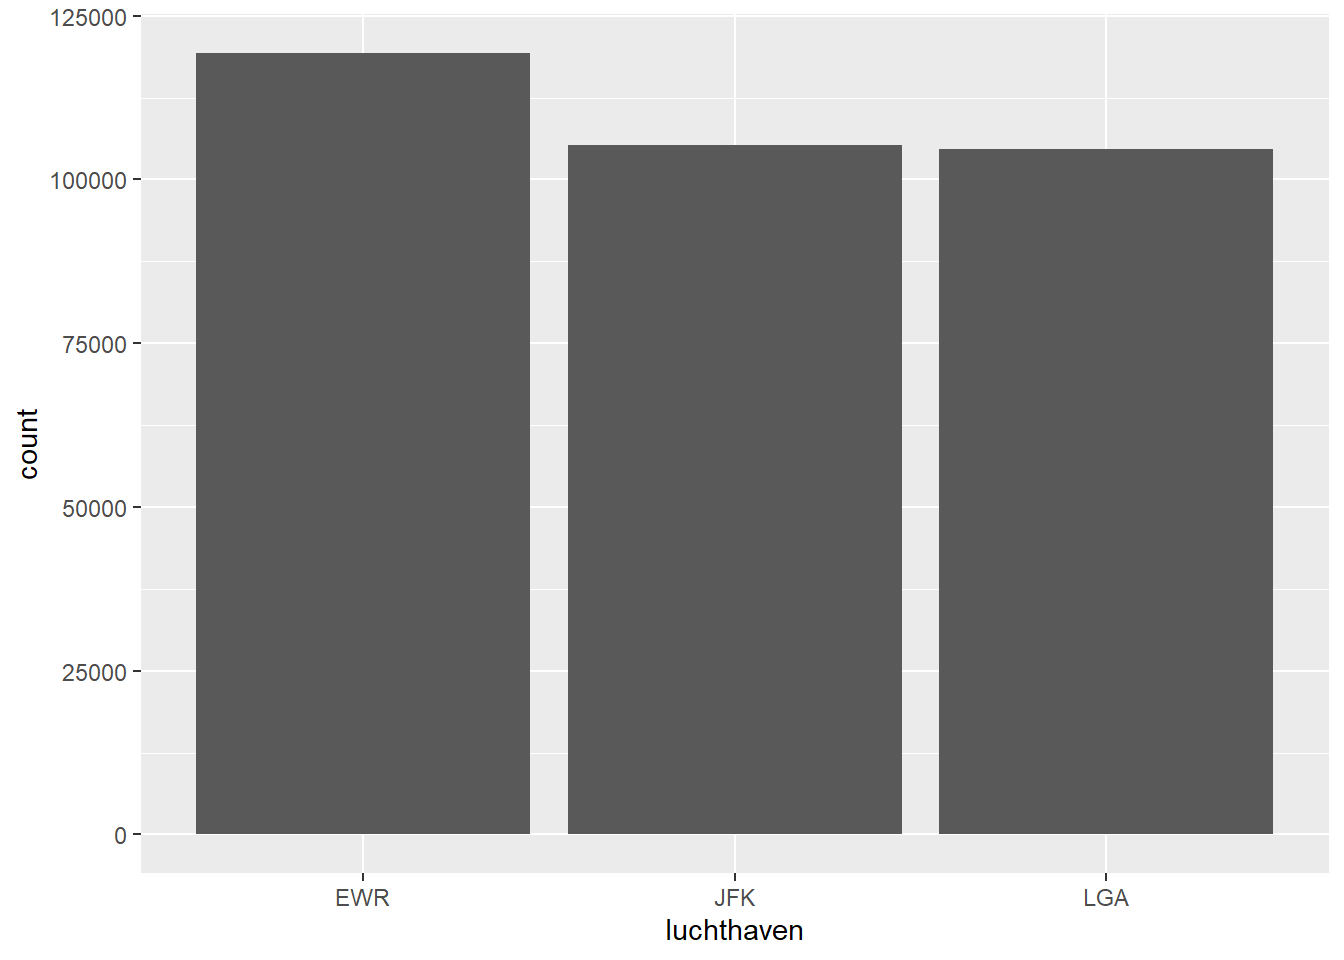
\includegraphics[width=0.49\linewidth]{lecture_notes_edda_files/figure-latex/2-3-1}
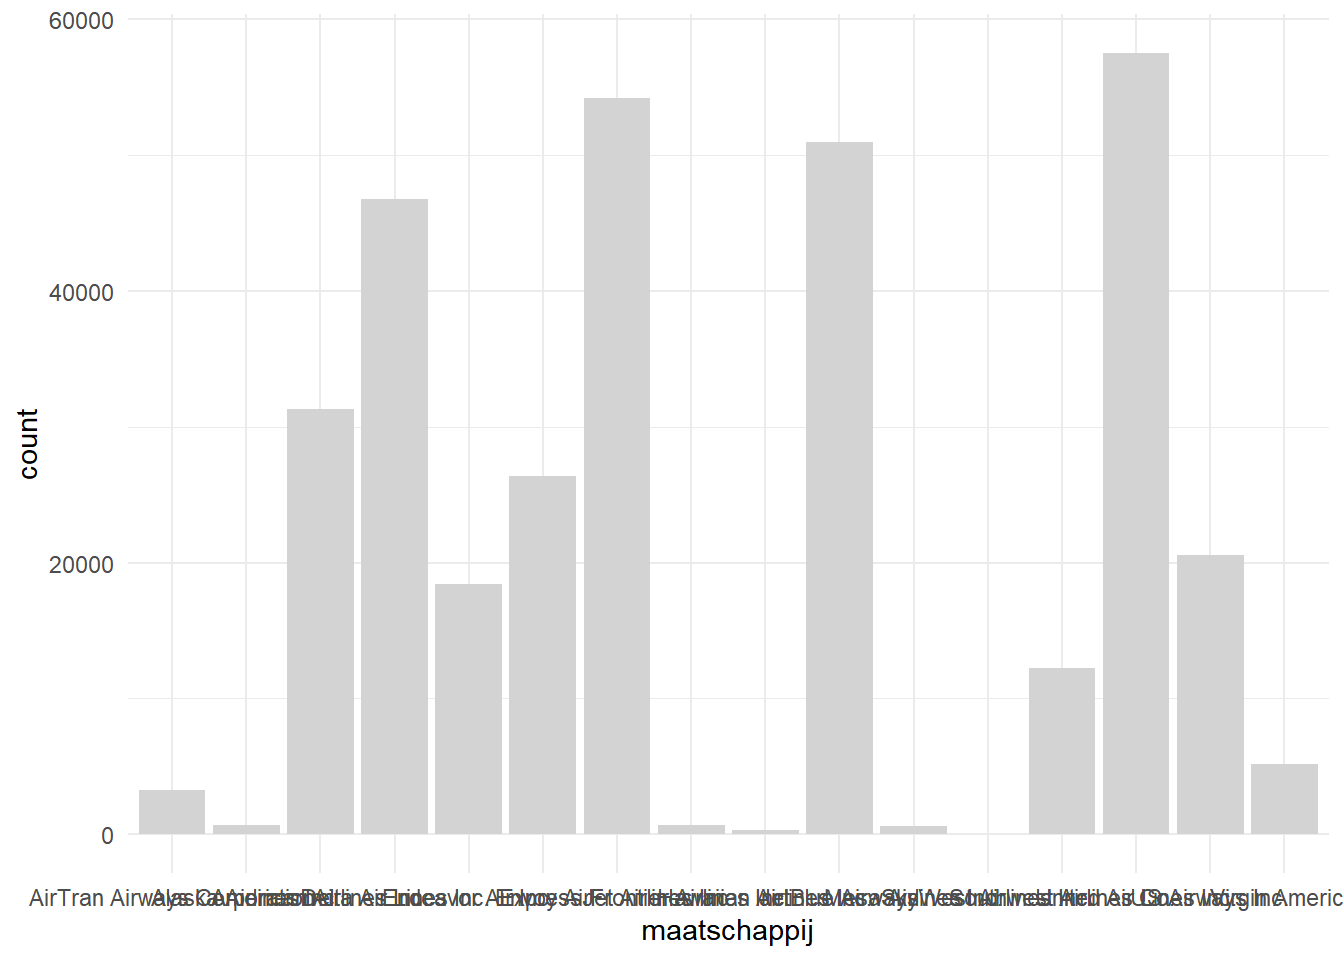
\includegraphics[width=0.49\linewidth]{lecture_notes_edda_files/figure-latex/2-3-2}
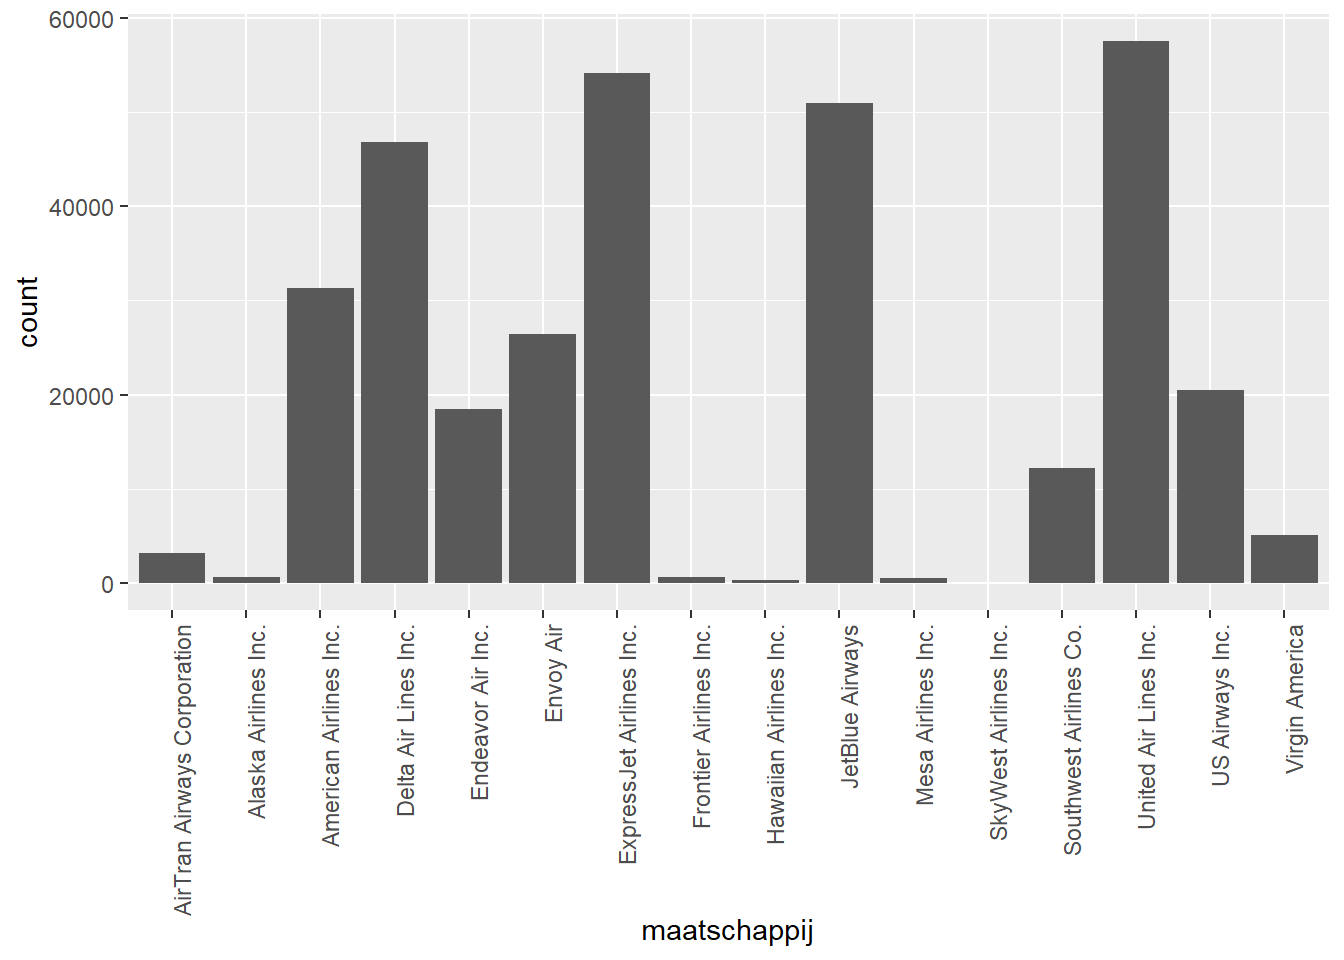
\includegraphics[width=0.49\linewidth]{lecture_notes_edda_files/figure-latex/2-3-3}
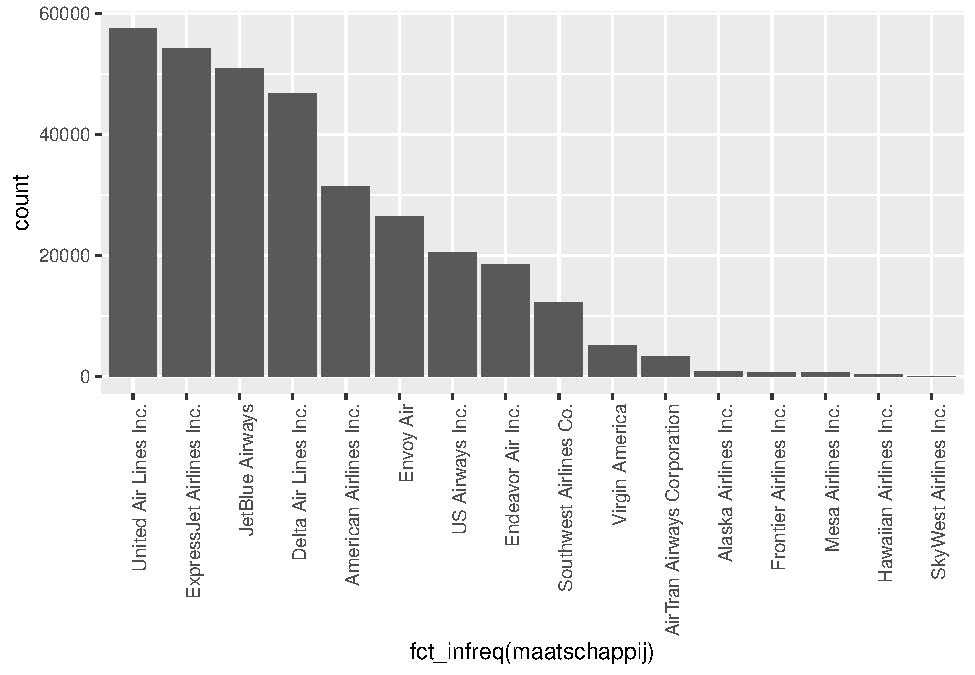
\includegraphics[width=0.49\linewidth]{lecture_notes_edda_files/figure-latex/2-3-4}

\begin{itemize}
\tightlist
\item
  Horizontale barplot

  \begin{itemize}
  \tightlist
  \item
    Zelfde principe als verticale barplots, maar dan met horizontale balken.
  \end{itemize}
\end{itemize}

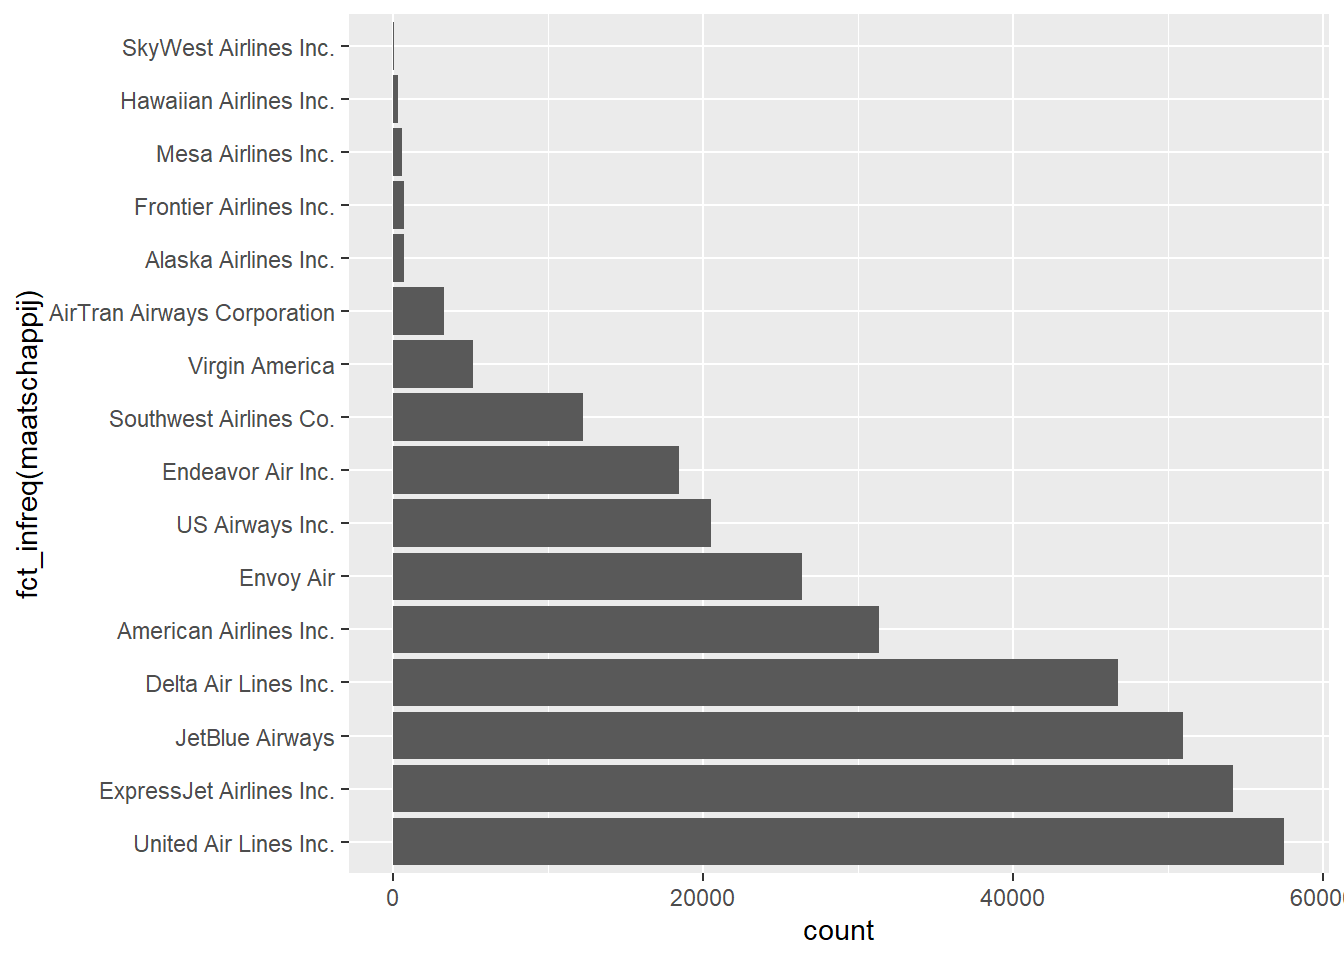
\includegraphics[width=0.49\linewidth]{lecture_notes_edda_files/figure-latex/2-4-1}

\begin{itemize}
\tightlist
\item
  Verticale/Horizontale dotplot

  \begin{itemize}
  \tightlist
  \item
    In plaats van balken te gebruiken om de frequentie van een waarde aan te geven, kan je dit ook met punten doen.
  \item
    Een dotplot laat duidelijker zien waar de sprongen in de verdeling zit. Daarom is de dotplot vooral relevant als je de waarden ordent volgens frequentie.
  \item
    Net als de barplot kan je zowel een verticale als horizontale dotplot maken.
  \end{itemize}
\end{itemize}

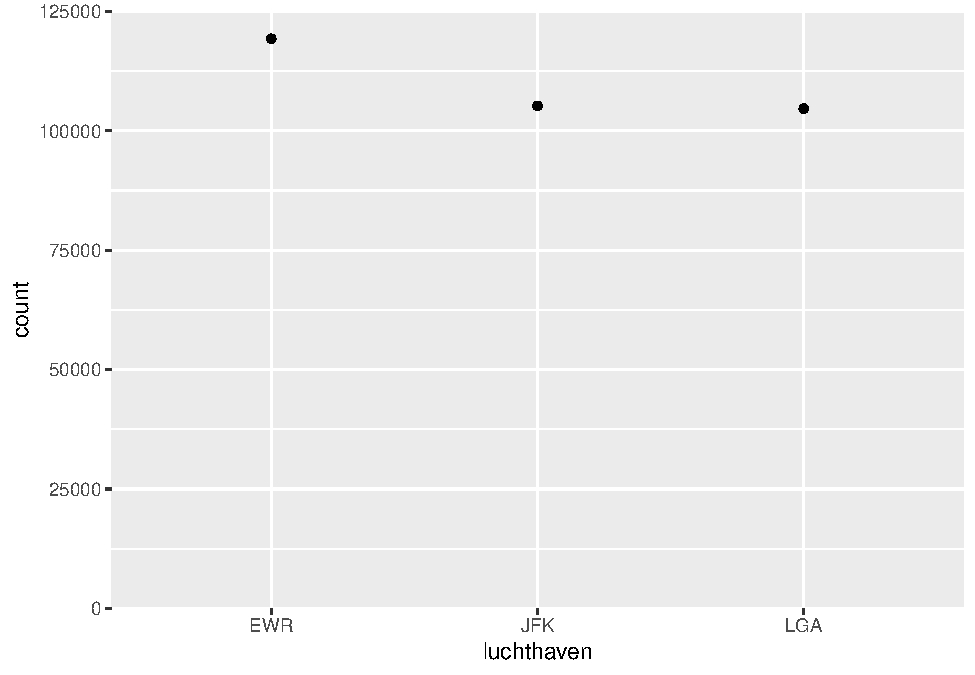
\includegraphics[width=0.49\linewidth]{lecture_notes_edda_files/figure-latex/2-5-1}
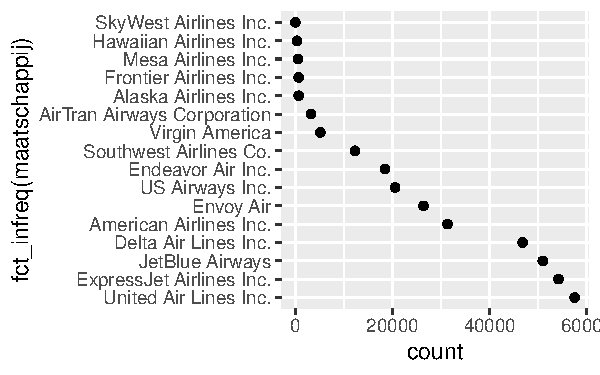
\includegraphics[width=0.49\linewidth]{lecture_notes_edda_files/figure-latex/2-5-2}

\begin{itemize}
\tightlist
\item
  Stacked barplot

  \begin{itemize}
  \tightlist
  \item
    We maken nu slechts 1 kolom. Iedere waarde is een andere kleur en neemt een deel van de balk in beslag. De volledige balk stelt 100\% van de data voor.
  \item
    Kan nuttig zijn om data cumulatief te bestuderen.
  \item
    Hiermee kunnen we vragen beantwoorden zoals: ``Welke waarden moeten we nemen om met zo weinig mogelijk waarden x\% van de objecten te hebben?''
  \end{itemize}
\end{itemize}

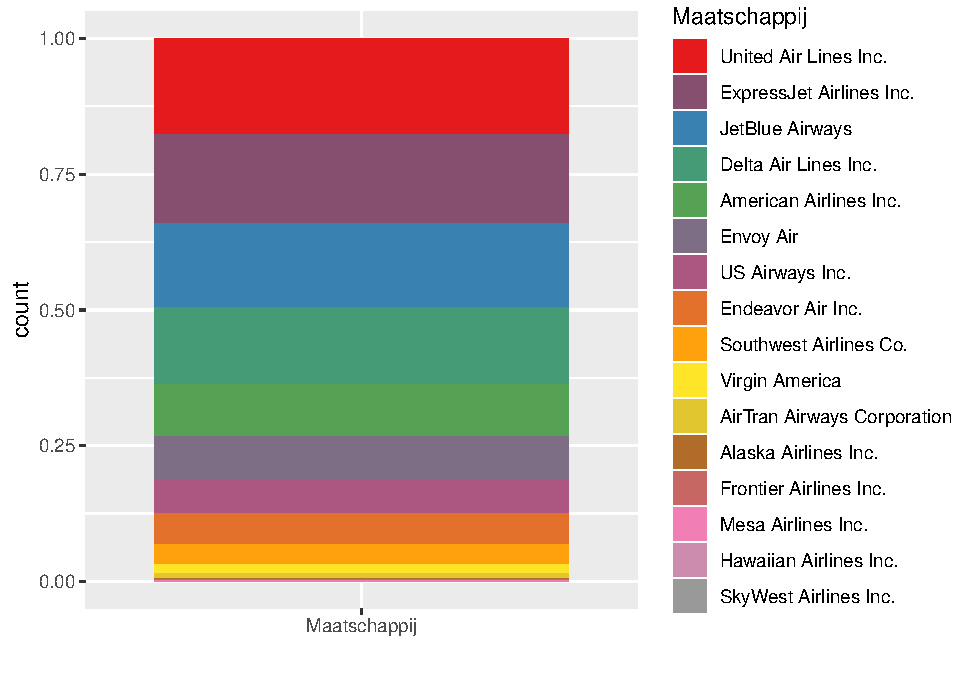
\includegraphics[width=0.49\linewidth]{lecture_notes_edda_files/figure-latex/2-6-1}

\begin{itemize}
\tightlist
\item
  Waarom geen pie charts?

  \begin{itemize}
  \tightlist
  \item
    Moeilijk te interpreteren.
  \item
    Verschillen tussen waarden zijn enkel duidelijk bij grote verschillen, terwijl barplots en dotplots deze ook bij kleine verschillen kunnen tonen.
  \item
    Voor cumulatieve analyses van de data zijn stacked barplots beter omdat het hier eenvoudiger is om af te leiden waar x\% zicht bevindt.
  \end{itemize}
\end{itemize}

\hypertarget{continue-variabele}{%
\subsection{Continue variabele}\label{continue-variabele}}

\begin{itemize}
\tightlist
\item
  Histogram

  \begin{itemize}
  \tightlist
  \item
    Analoog met barplot, alleen gaan we hier eerst onze ``categorieën'' definiëren.
  \item
    Dit wordt `binning' genoemd en wordt bepaald door een bin-breedte te kiezen.

    \begin{itemize}
    \tightlist
    \item
      Je kan de binbreedte rechtstreeks kiezen of bepalen door vast te leggen hoeveel categorieën/bins je wenst.
    \end{itemize}
  \item
    Voor de visualisatie, worden alle waarden gegroepeerd per `bin'.
  \item
    De binbreedte kan een enorme impact hebben op het uitzicht van de verdeling.

    \begin{itemize}
    \tightlist
    \item
      Hoe breder de bins, hoe minder modi je kan detecteren.
    \item
      Hoe smaller de bins, hoe meer modi je gaat zien, hoewel dit niet altijd even betekenisvol is.
    \item
      Hoe smaller de bins, hoe minder data er in iedere bin gaat zitten en dan kunnen patronen wel in jouw dataset bestaan maar louter ten gevolge van toeval.
    \end{itemize}
  \end{itemize}
\end{itemize}

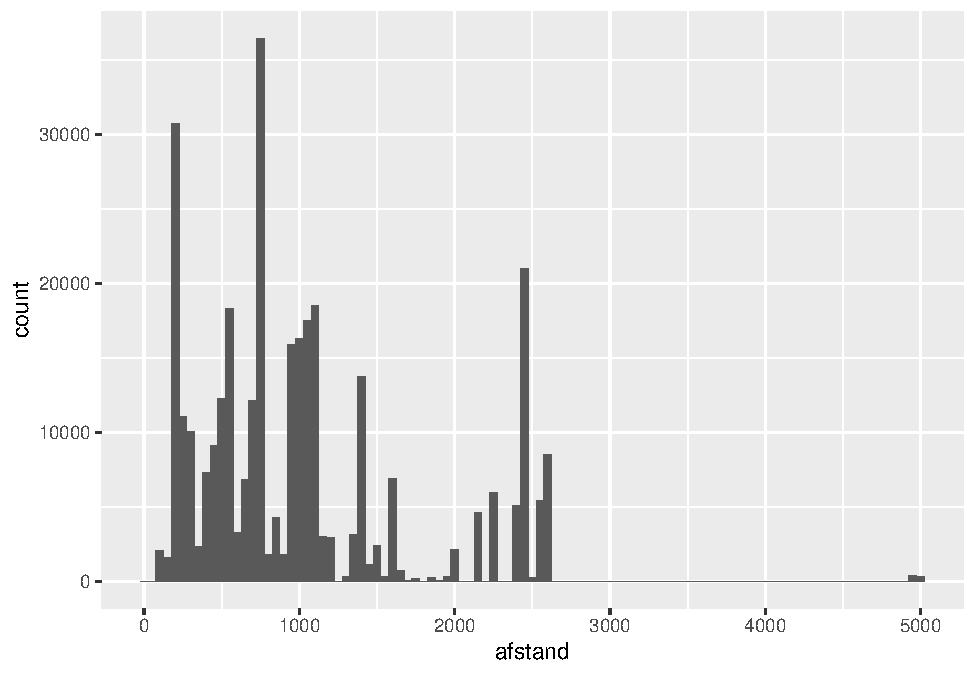
\includegraphics[width=0.49\linewidth]{lecture_notes_edda_files/figure-latex/2-7-1}
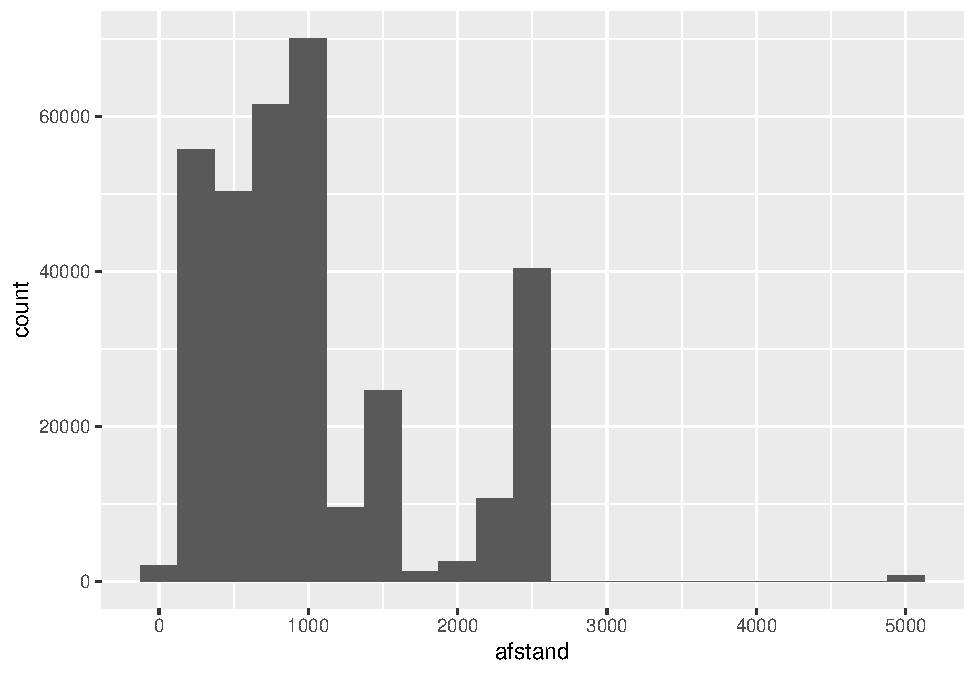
\includegraphics[width=0.49\linewidth]{lecture_notes_edda_files/figure-latex/2-7-2}
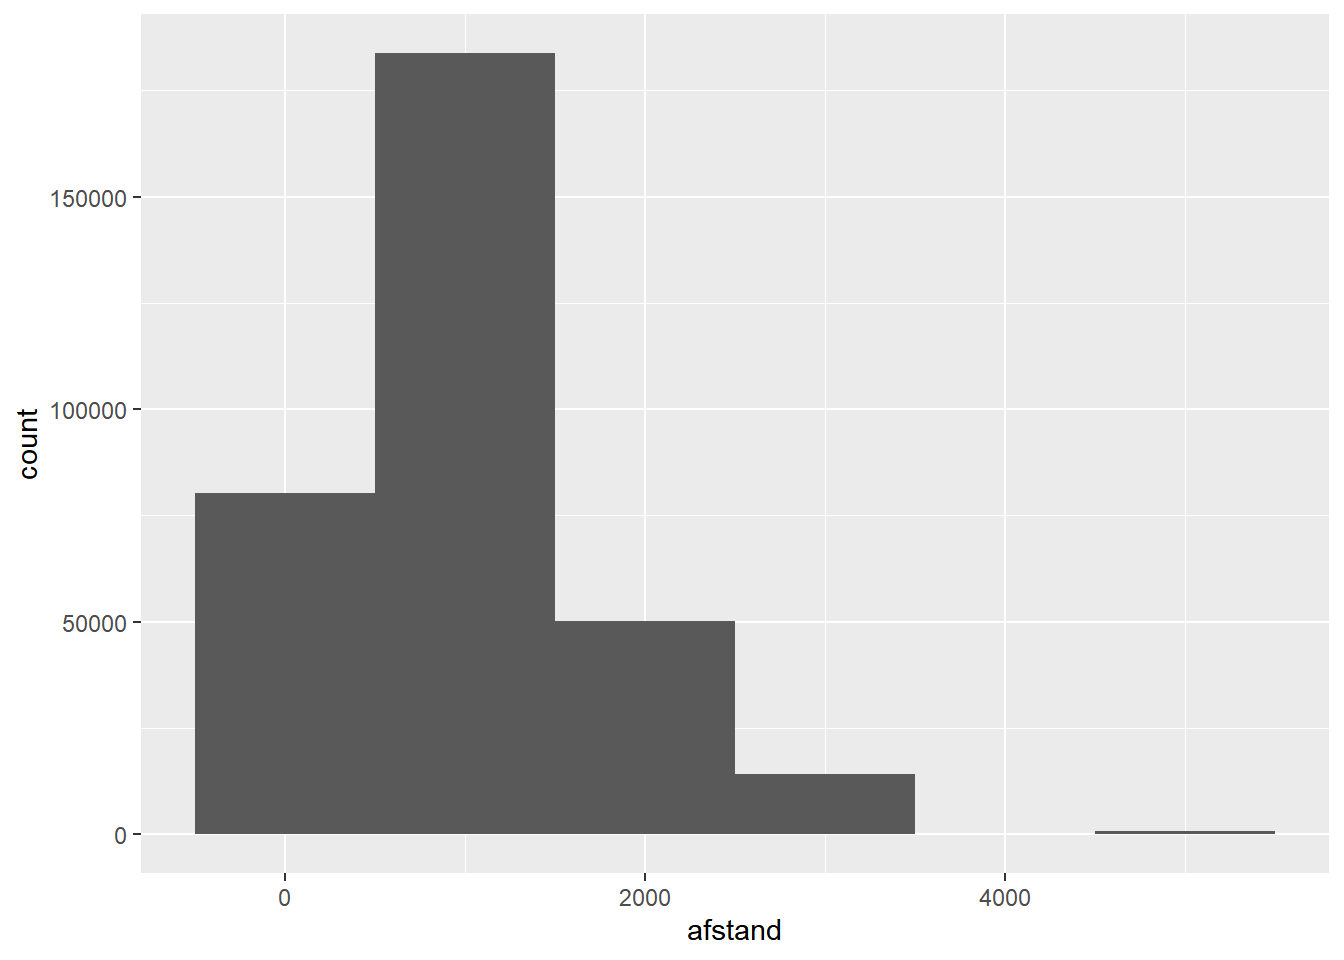
\includegraphics[width=0.49\linewidth]{lecture_notes_edda_files/figure-latex/2-7-3}

\begin{itemize}
\tightlist
\item
  Boxplot

  \begin{itemize}
  \tightlist
  \item
    De lijn in het midden duidt de mediaan aan. Dit betekent dat 50\% van je data onder deze lijn ligt, terwijl 50\% er boven ligt.
  \item
    De box in het midden duidt de middelste 50\% van je data aan. Dit wordt ook de interkwartiel-box genoemd. Dit betekent dat 25\% van je data onder deze box zit en nog eens 25\% boven deze box ligt. Hoe groter de box, des te meer de data gespreid is.
  \item
    Indien de box aan één zijde van de mediaanlijn groter is dan aan de andere zijde, dan wijst dit er op dat de data meer gespreid is aan die kant.
  \item
    De ``whiskers'' geven de laatste datapunten aan die als ``normaal'' beschouwd worden. Datapunten buiten deze grenzen beschouwt een boxplot als outliers of extreme waarden.

    \begin{itemize}
    \tightlist
    \item
      De grens waar data van normaal naar extreem overgaat wordt door de boxplot bepaald door anderhalf keer de grootte van de interkwartiel-box op te tellen (en af te trekken) van de bovenste (onderste) grens van de interkwartiel-box. Punten die hier buiten liggen zijn outliers en worden als aparte punten aangeduid. De whiskers zelf duiden de laatste datapunten aan binnen deze grenzen.
    \end{itemize}
  \end{itemize}
\end{itemize}

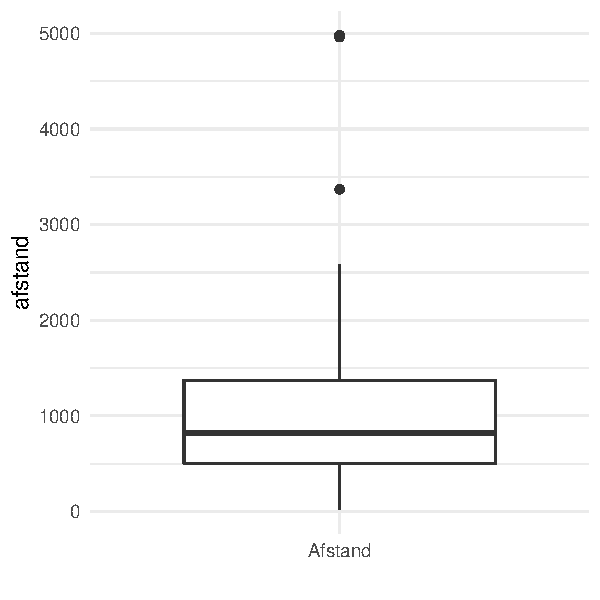
\includegraphics[width=0.49\linewidth]{lecture_notes_edda_files/figure-latex/2-8-1}

\begin{itemize}
\tightlist
\item
  Het is niet abnormaal dat er outliers in je data aanwezig zijn.
\item
  Bij normaal verdeelde data zal je gemiddeld 7 outliers per 1000 datapunten mogen verwachten.

  \begin{itemize}
  \tightlist
  \item
    Een normale verdeling is een bepaalde manier waarop data waarden verdeeld kunnen zijn die in de realiteit vaak voorkomt.
  \end{itemize}
\item
  Indien je echter veel meer outliers ziet op je boxplot visualisatie, dan is de kans reëel dat er meer aan de hand is:

  \begin{itemize}
  \tightlist
  \item
    Er zijn bijvoorbeeld systematische meetfouten
  \item
    De objecten in je data zijn in feite op bepaalde aspecten significant verschillend waardoor je ze apart zou moeten bestuderen.
  \end{itemize}
\end{itemize}

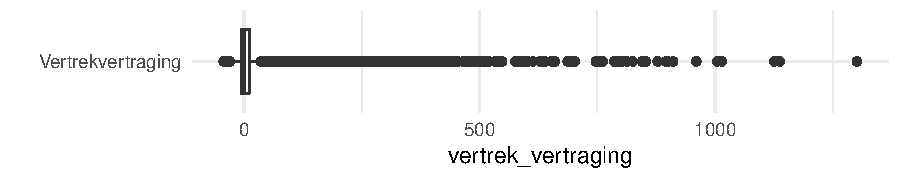
\includegraphics[width=0.49\linewidth]{lecture_notes_edda_files/figure-latex/2-9-1}

\begin{itemize}
\tightlist
\item
  Violinplot

  \begin{itemize}
  \tightlist
  \item
    Een violinplot kan je beschouwen als een combinatie van een histogram en een boxplot.
  \item
    Net als bij een boxplot wordt op verticale wijze getoond hoe de data verspreid is.
  \item
    Net als bij een histogram kan je goed zien waar het volume (de massa) van de data zich bevindt.
  \item
    Net als bij een histogram kan je detecteren hoeveel modi de data bezit.
  \item
    In tegenstelling tot de boxplot, kan je bij een violinplot wel niet duidelijk zien waar bijvoorbeeld het `midden' van je data is.
  \end{itemize}
\end{itemize}

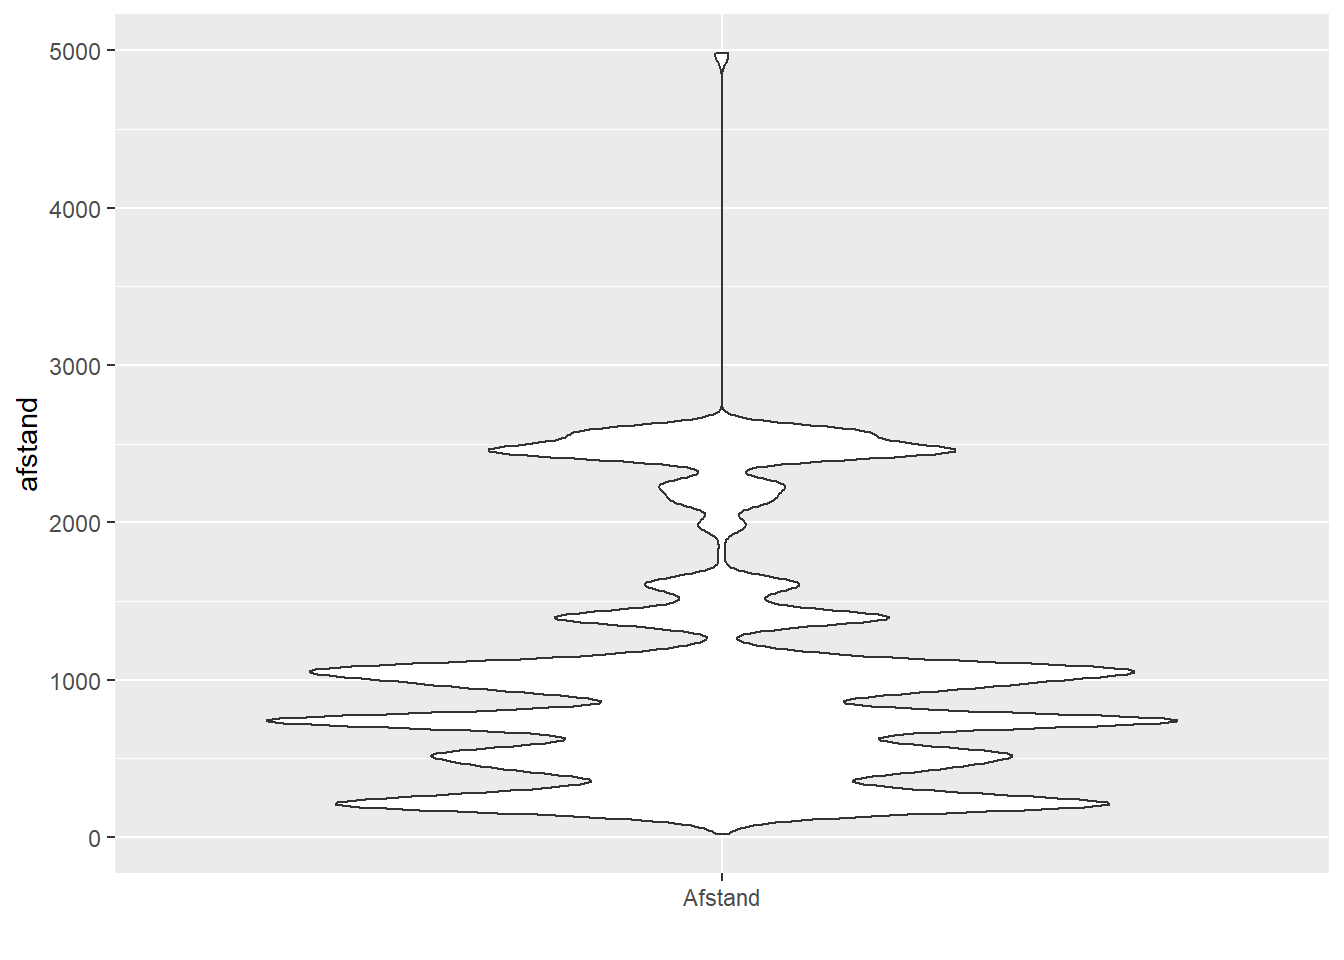
\includegraphics[width=0.49\linewidth]{lecture_notes_edda_files/figure-latex/2-10-1}
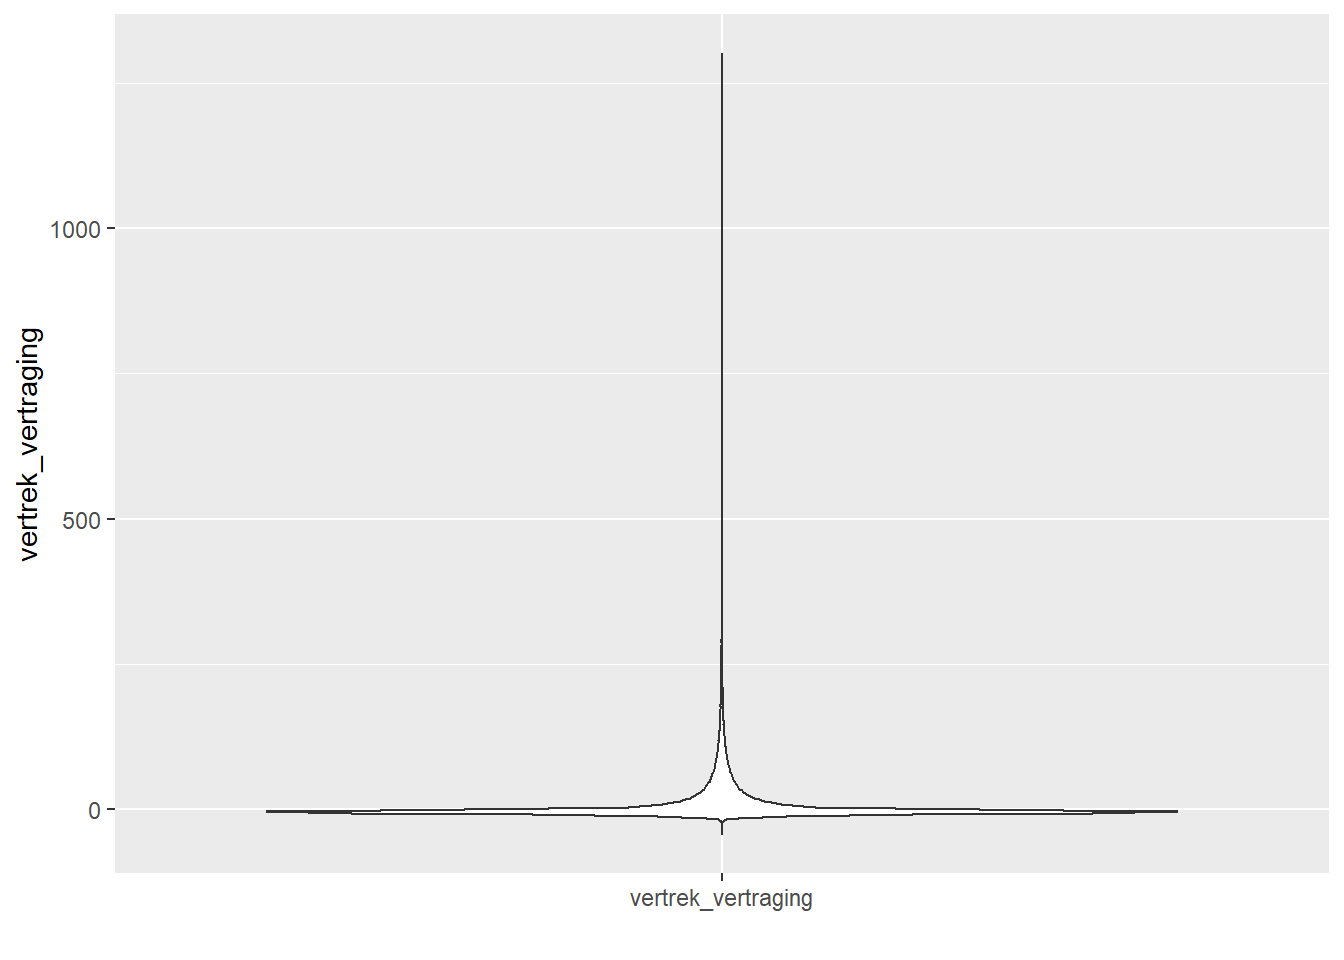
\includegraphics[width=0.49\linewidth]{lecture_notes_edda_files/figure-latex/2-10-2}

\hypertarget{datavisualisatie-van-2-variabelen}{%
\section{Datavisualisatie van 2 variabelen}\label{datavisualisatie-van-2-variabelen}}

\begin{itemize}
\tightlist
\item
  Van zodra er twee variabelen zijn, gaan we op zoek naar patronen in relaties tussen twee variabelen.
\item
  Het is belangrijk en essentieel te beseffen dat mensen een automatische reflex hebben om te denken in termen van oorzaak-gevolg als we kijken naar relaties tussen twee variabelen.

  \begin{itemize}
  \tightlist
  \item
    Het is echter niet omdat er een duidelijke relatie bestaat tussen twee variabelen (correlatie), dat hier sprake is van een oorzaak-gevolg verband (causaliteit).

    \begin{itemize}
    \tightlist
    \item
      Bijvoorbeeld: Indien in de zomer de verkoop van paraplu's sterk stijgt, dan zal de graanopbrengst in het najaar dalen. Dit betekent niet dat de verkoop van paraplu's een impact heeft op de graanopbrengst. Wat hier waarschijnlijk gebeurt, is dat door hevige regenval in de zomermaanden, de verkoop van paraplu's is toegenomen en de graanoogst tegenvalt.
    \item
      Soms is het intuïtief zeer onwaarschijnlijk dat de waargenomen correlatie causaliteit impliceert. Kijk hiervoor maar eens naar de voorbeelden op \url{http://www.tylervigen.com/spurious-correlations}
    \item
      Wanneer het echter plausibel is dat de waargenomen correlatie causaliteit voorstelt, is het belangrijk dat we tegen onze natuurlijke reflex in gaan en niet in termen van oorzaak-gevolg denken.
    \item
      Het aantonen van causaliteit is nooit mogelijk met descriptieve en exploratieve data analyse!
    \end{itemize}
  \end{itemize}
\item
  Toch helpt het bij het maken van een datavisualisatie met 2 variabelen te denken in termen van oorzaak-gevolg, ook al weten we dat we dit nooit mogen concluderen!

  \begin{itemize}
  \tightlist
  \item
    De variabele die we het label ``oorzaak'' geven, zullen we voortaan ``onafhankelijke variabele'' noemen.
  \item
    De variabele die we het label ``gevolg'' geven, zullen we voortaan ``afhankelijke variabele'' noemen.
  \end{itemize}
\item
  Waar we eigenlijk in geïnteresseerd zijn bij een visualisatie van 2 variabelen is de impact van de onafhankelijke variabele op de afhankelijke variabele weer te geven.
\item
  Alle vragen die we kunnen stellen bij de visualisatie van 1 variabele, kunnen we nog steeds stellen, met telkens de bijkomende vraag of het waargenomen patroon verandert als de onafhankelijke variabele van waarde verandert.
\end{itemize}

\hypertarget{situatie-1-de-onafhankelijke-variabele-is-categorisch}{%
\subsection{Situatie 1: De onafhankelijke variabele is categorisch}\label{situatie-1-de-onafhankelijke-variabele-is-categorisch}}

\begin{itemize}
\tightlist
\item
  Oplossing 1: Meerdere univariate plots per waarde van de onafhankelijke variabele

  \begin{itemize}
  \tightlist
  \item
    WBij een categorische onafhankelijke variabele kan je altijd aparte univaraite visualisaties maken van de afhankelijke variabele, per mogelijke waarde van de onafhankelijke variabele.
  \item
    Om dit soort plots zo betekenisvol mogelijk te maken, moet je er voor zorgen dat het eenvoudig is patronen te vergelijken tussen verschillende waarden van de onafhankelijke variabele. Daarom respecteer je best volgende tips:

    \begin{itemize}
    \tightlist
    \item
      Plaats de verschillende plots in een intuïtief logische volgorde (natuurlijke volgorde bij ordinale onafhankelijke variabele, alfabetisch bij nominale variabele, \ldots{})
    \item
      Gebruik dezelfde schalen op de assen in iedere plot
    \end{itemize}
  \end{itemize}
\end{itemize}

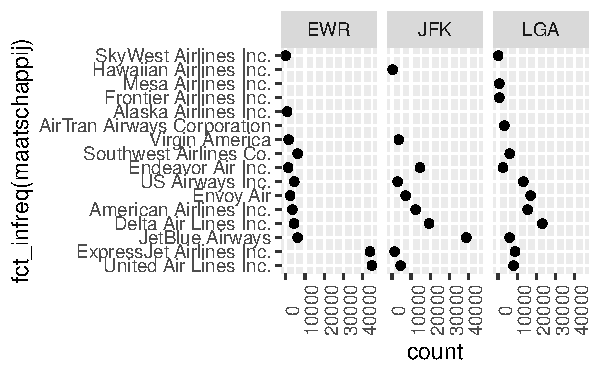
\includegraphics[width=0.49\linewidth]{lecture_notes_edda_files/figure-latex/2-11-1}
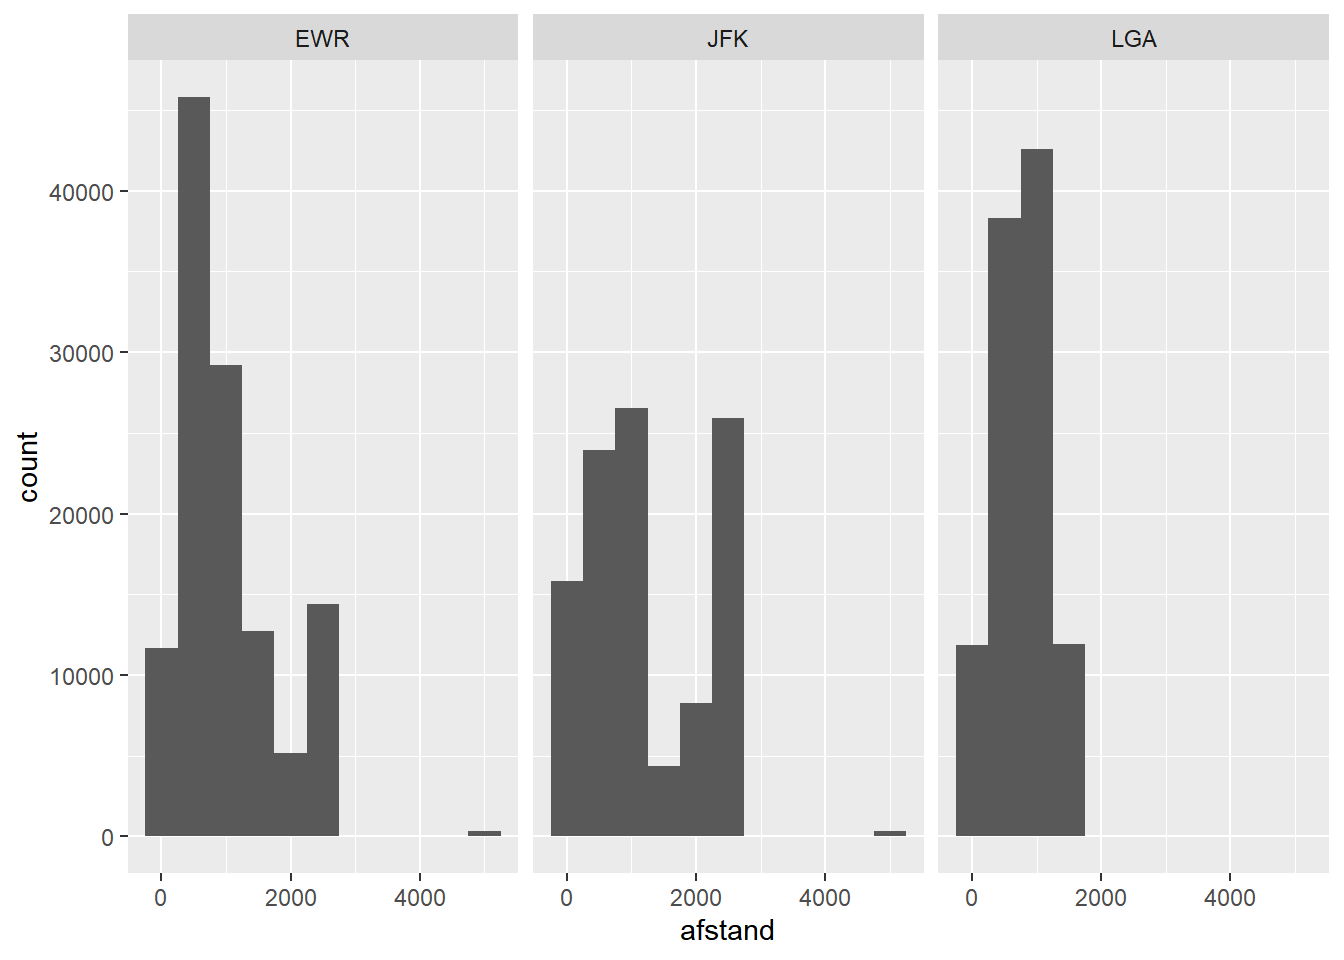
\includegraphics[width=0.49\linewidth]{lecture_notes_edda_files/figure-latex/2-11-2}
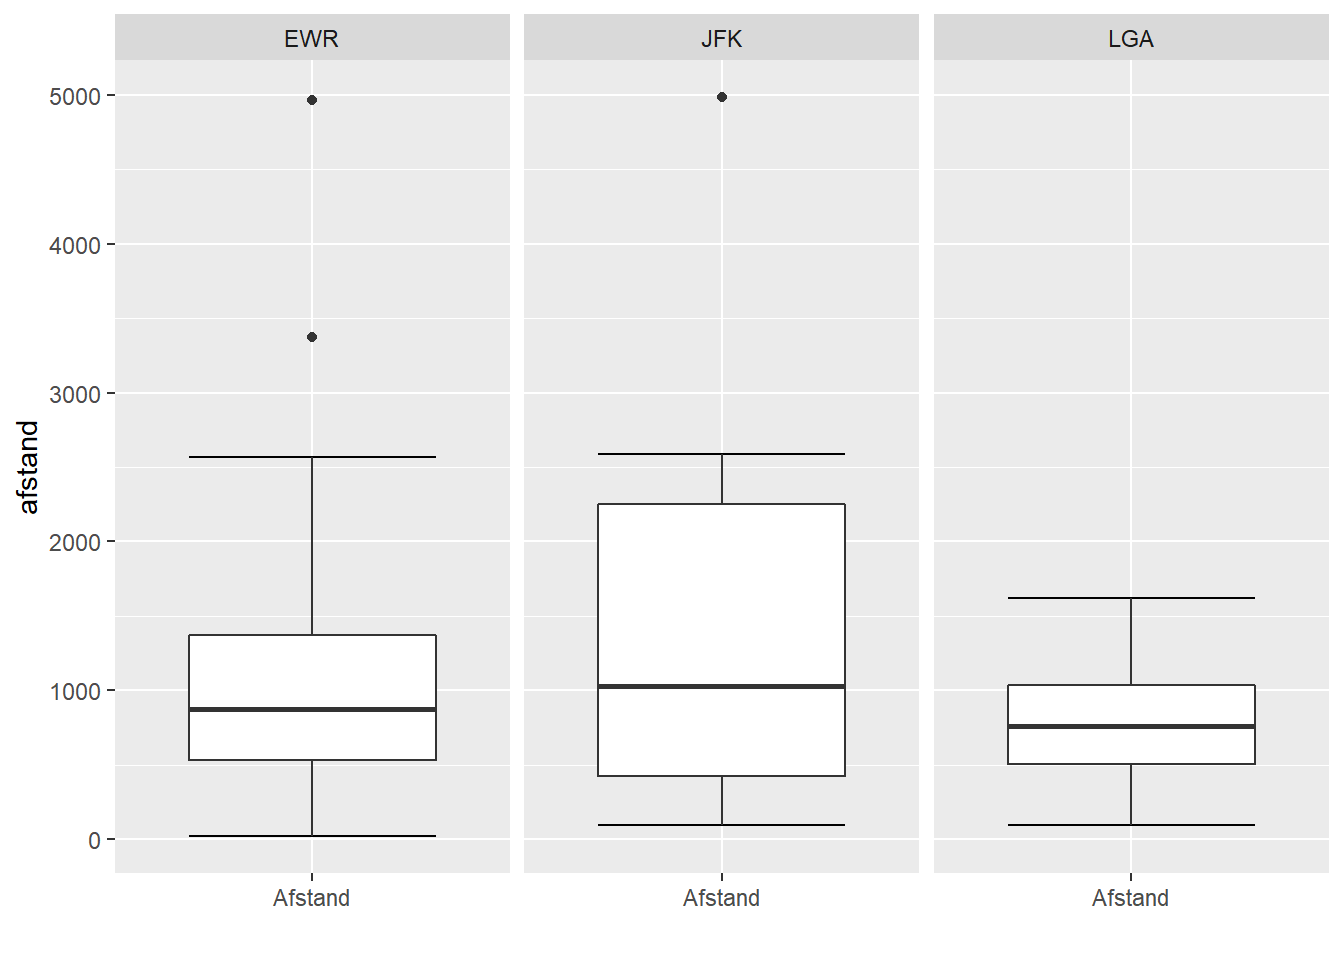
\includegraphics[width=0.49\linewidth]{lecture_notes_edda_files/figure-latex/2-11-3}
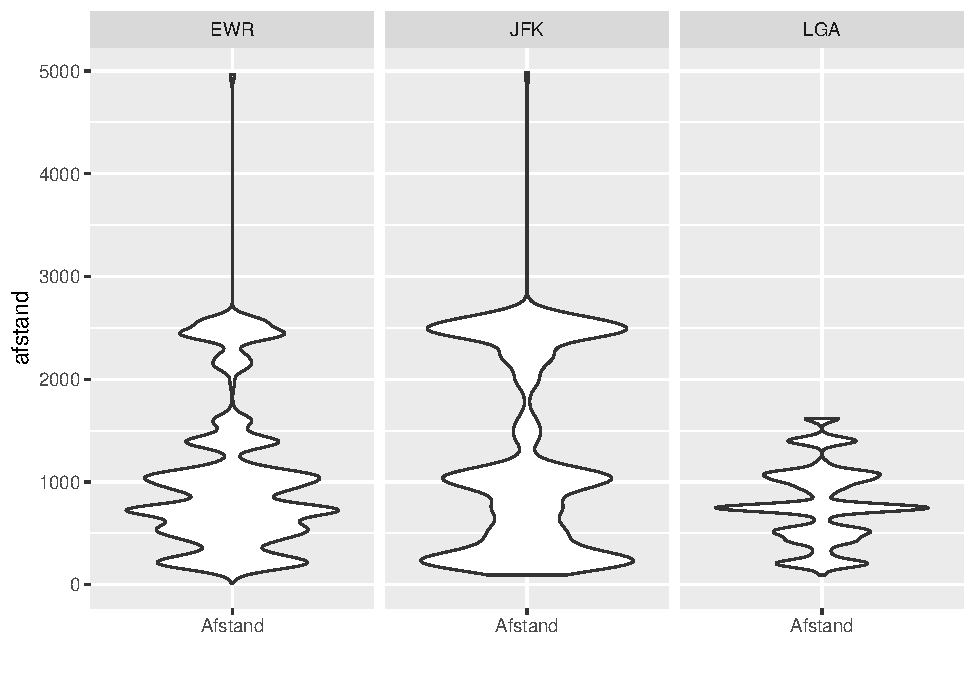
\includegraphics[width=0.49\linewidth]{lecture_notes_edda_files/figure-latex/2-11-4}

\begin{itemize}
\tightlist
\item
  Oplossing 2: 1 bivariate plot

  \begin{itemize}
  \tightlist
  \item
    In dit geval plaats je de onafhankelijke variabele altijd op de X-as!
  \item
    Indien de afhankelijke variabele een categorische variabele is:

    \begin{itemize}
    \tightlist
    \item
      Kan je meerdere barplots op 1 grafiek visualiseren, met telkens de bars gegroepeerd per waarde van de onafhankelijke variabele.
    \item
      Kan je meerdere stacked barplots op 1 grafiek plaatsen, met telkens een volledige stack per waarde van de onafhankelijke variabele.
    \end{itemize}
  \item
    Indien de afhankelijke variabele een continue variabele is:

    \begin{itemize}
    \tightlist
    \item
      Kan je meerdere boxplots op 1 grafiek visualiseren, met telkens 1 boxplot per waarde van de onafhankelijke variabele.
    \item
      Kan je meerdere violinplots op 1 grafiek tonen, met telkens 1 violinplot per waarde van de onafhankelijke variabele.
    \end{itemize}
  \end{itemize}
\end{itemize}

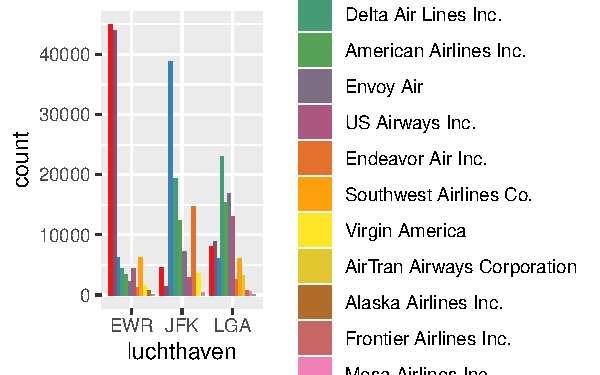
\includegraphics[width=0.49\linewidth]{lecture_notes_edda_files/figure-latex/2-12-1}
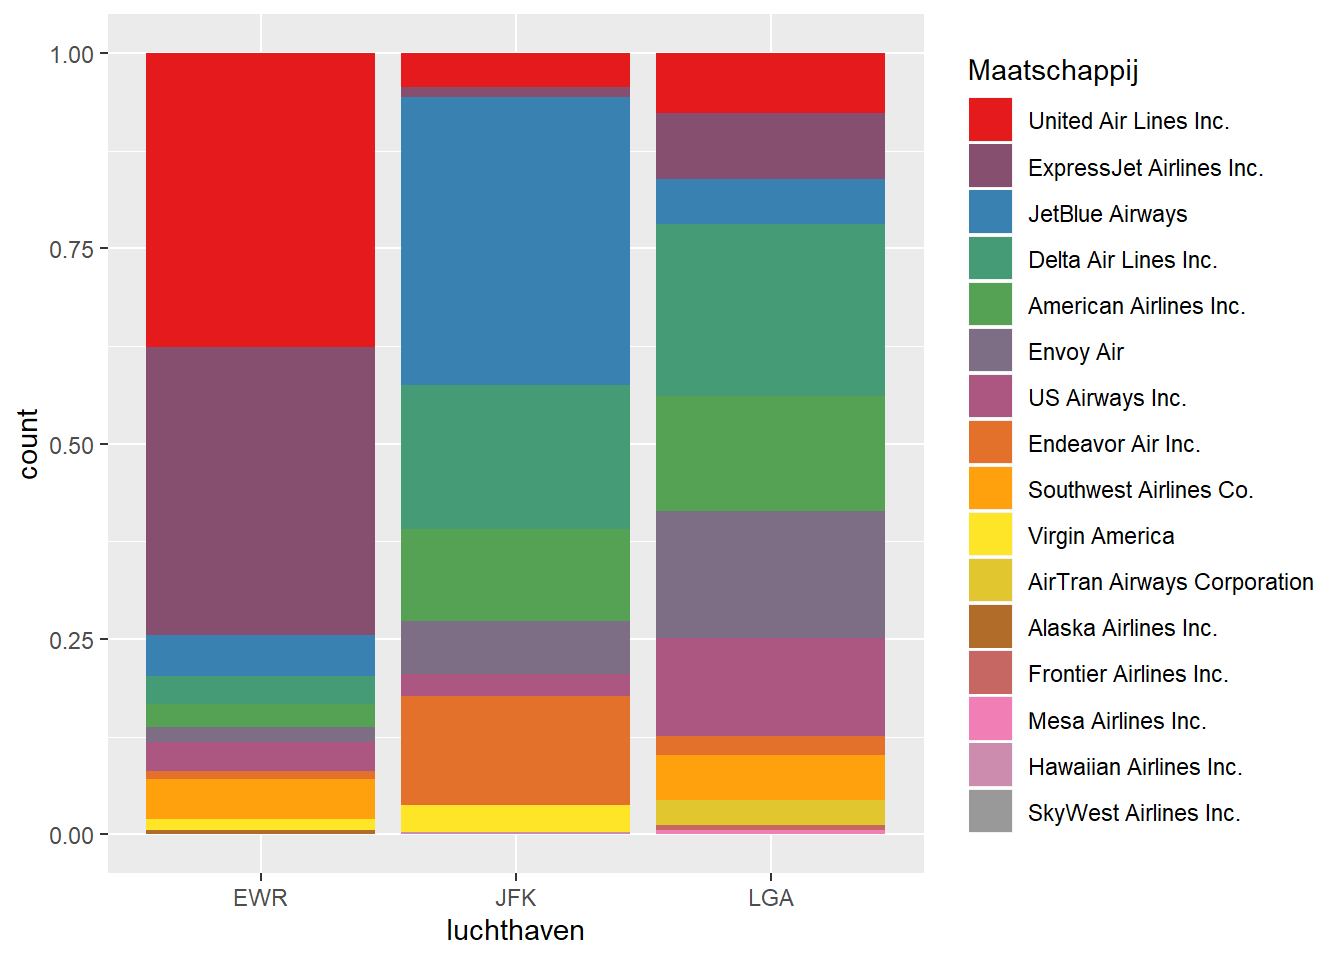
\includegraphics[width=0.49\linewidth]{lecture_notes_edda_files/figure-latex/2-12-2}
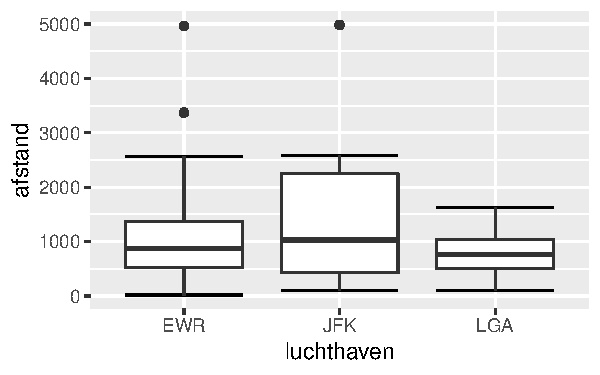
\includegraphics[width=0.49\linewidth]{lecture_notes_edda_files/figure-latex/2-12-3}
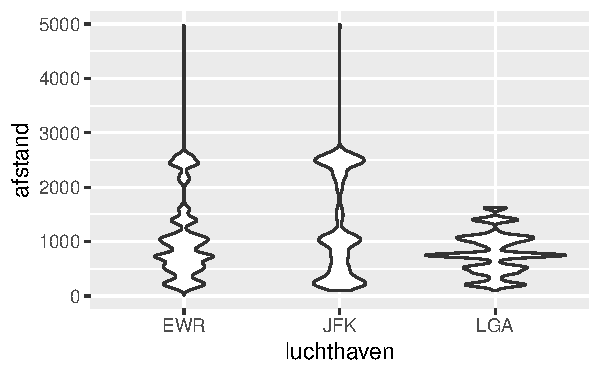
\includegraphics[width=0.49\linewidth]{lecture_notes_edda_files/figure-latex/2-12-4}
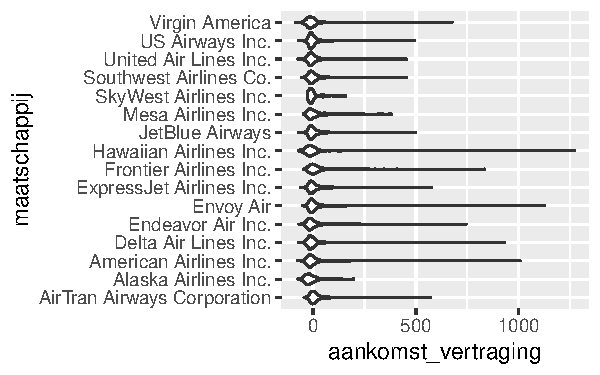
\includegraphics[width=0.49\linewidth]{lecture_notes_edda_files/figure-latex/2-12-5}

\hypertarget{situatie-2-de-onafhankelijke-variabele-is-continue}{%
\subsection{Situatie 2: De onafhankelijke variabele is continue}\label{situatie-2-de-onafhankelijke-variabele-is-continue}}

\begin{itemize}
\tightlist
\item
  In dit geval kan je geen aparte plot per mogelijke waarde van de onafhankelijke variabele maken omdat er mogelijk oneindig veel waarden zijn.
\item
  Indien de afhankelijke variabele continu is, dan kan je een scatterplot maken.

  \begin{itemize}
  \tightlist
  \item
    Iedere observatie is een punt in je grafiek, waarbij de x-waarde op de grafiek overeenkomt met de waarde van de onafhankelijke variabele en de y-waarde op de grafiek overeenkomt met de waarde van de afhankelijke variabele.

    \begin{itemize}
    \tightlist
    \item
      Om patronen beter te herkennen kan je een ``trend-lijn'' toevoegen.
    \end{itemize}
  \end{itemize}
\item
  Indien de afhankelijke variabele categorisch is, dan kan je niet rechtstreeks een betekenisvolle plot maken omdat er waarschijnlijk te weinig datapunten zijn voor iedere mogelijke waarde van de onafhankelijke variabele.

  \begin{itemize}
  \tightlist
  \item
    Wat je dan best kan doen, is de onafhankelijke continue variabele categorisch maken door bins te definiëren. En dan ben je terug in de situatie waarbij de onafhankelijke variabele categorisch is.
  \end{itemize}
\end{itemize}

\begin{verbatim}
## `geom_smooth()` using method = 'gam' and formula 'y ~ s(x, bs = "cs")'
\end{verbatim}

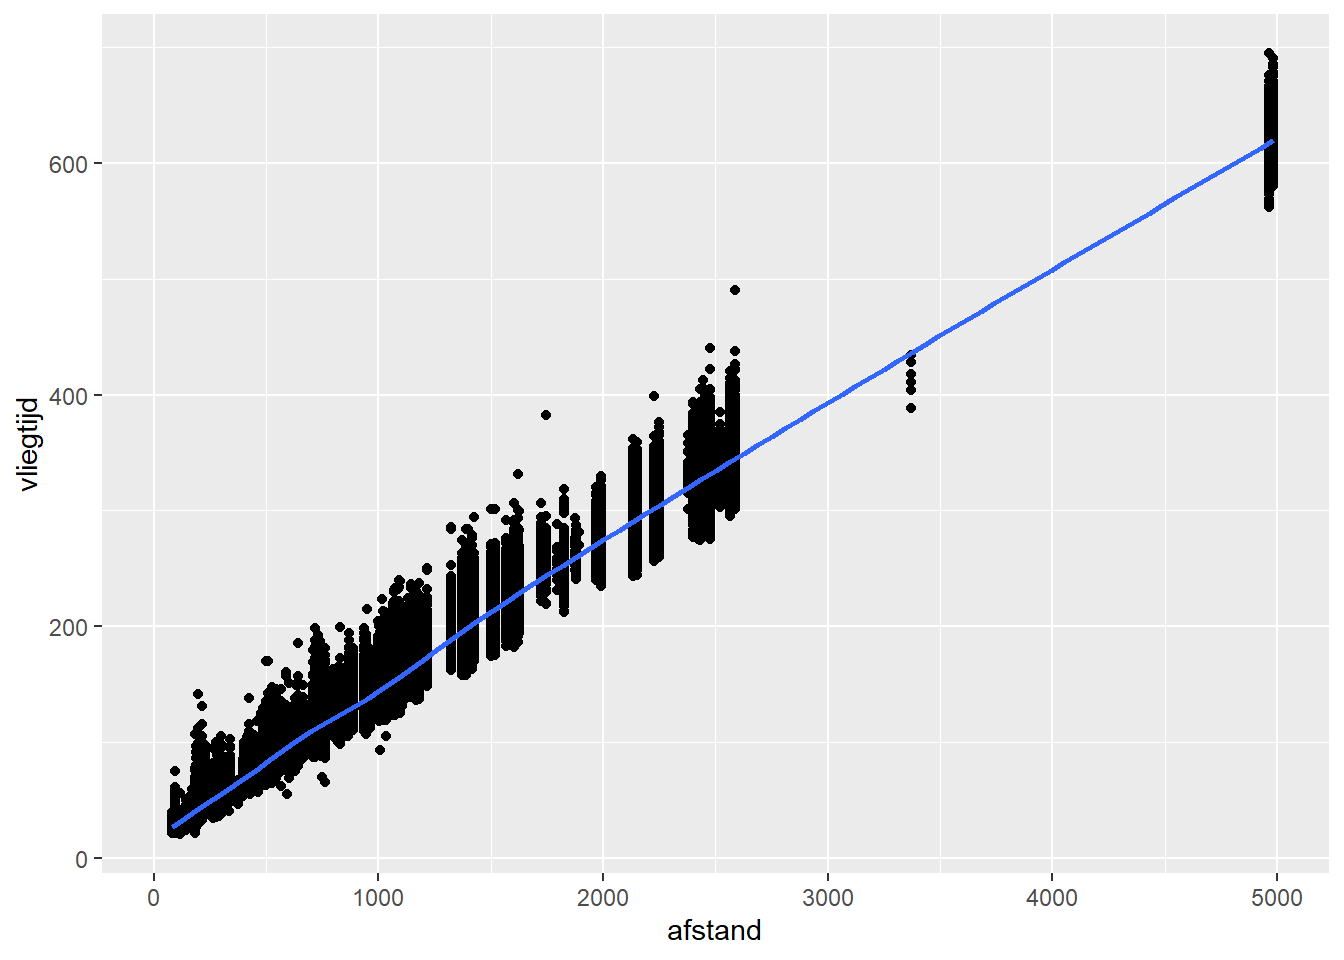
\includegraphics[width=0.49\linewidth]{lecture_notes_edda_files/figure-latex/2-13-1}

\hypertarget{situatie-3-de-onafhankelijke-variabele-stelt-de-tijd-voor}{%
\subsection{Situatie 3: De onafhankelijke variabele stelt de tijd voor}\label{situatie-3-de-onafhankelijke-variabele-stelt-de-tijd-voor}}

\begin{itemize}
\tightlist
\item
  Dit is een specifieke situatie waarbij je de onafhankelijke variabele zowel als een continue en als een categorische variabele kunt beschouwen.
\item
  Hoe nauwkeuriger de tijdmeting, des te groter het continue karakter van de data.
\item
  Op zich kan je bovenstaande visualisaties dus ook maken met een onafhankelijke variabele die de tijd voorstelt. Hierbij stelt de X-as nu de tijd voor.
\end{itemize}

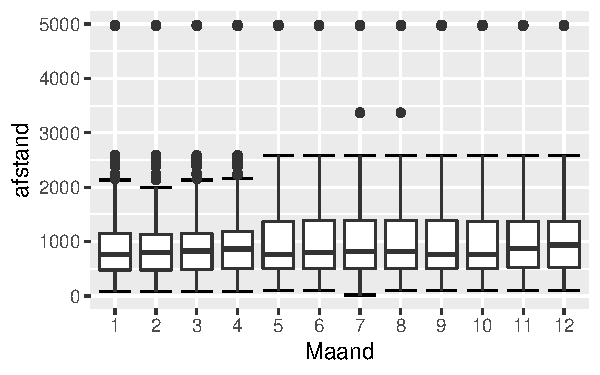
\includegraphics[width=0.49\linewidth]{lecture_notes_edda_files/figure-latex/2-14-1}
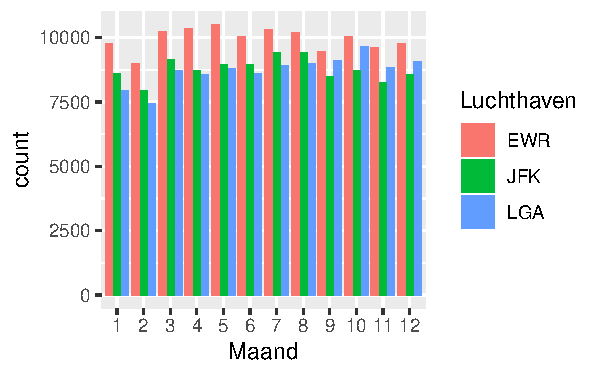
\includegraphics[width=0.49\linewidth]{lecture_notes_edda_files/figure-latex/2-14-2}

\begin{itemize}
\tightlist
\item
  Er is echter een specifieke situatie waarbij een betere visualisatie mogelijk is, namelijk wanneer er op ieder mogelijk tijdstip slechts 1 observatie is.

  \begin{itemize}
  \tightlist
  \item
    Dit doet zich voor als men bijvoorbeeld op ieder uur van de dag de temperatuur opneemt in Ukkel.
  \item
    In zulke gevallen kan men best een lijn-plot gebruiken.
  \end{itemize}
\end{itemize}

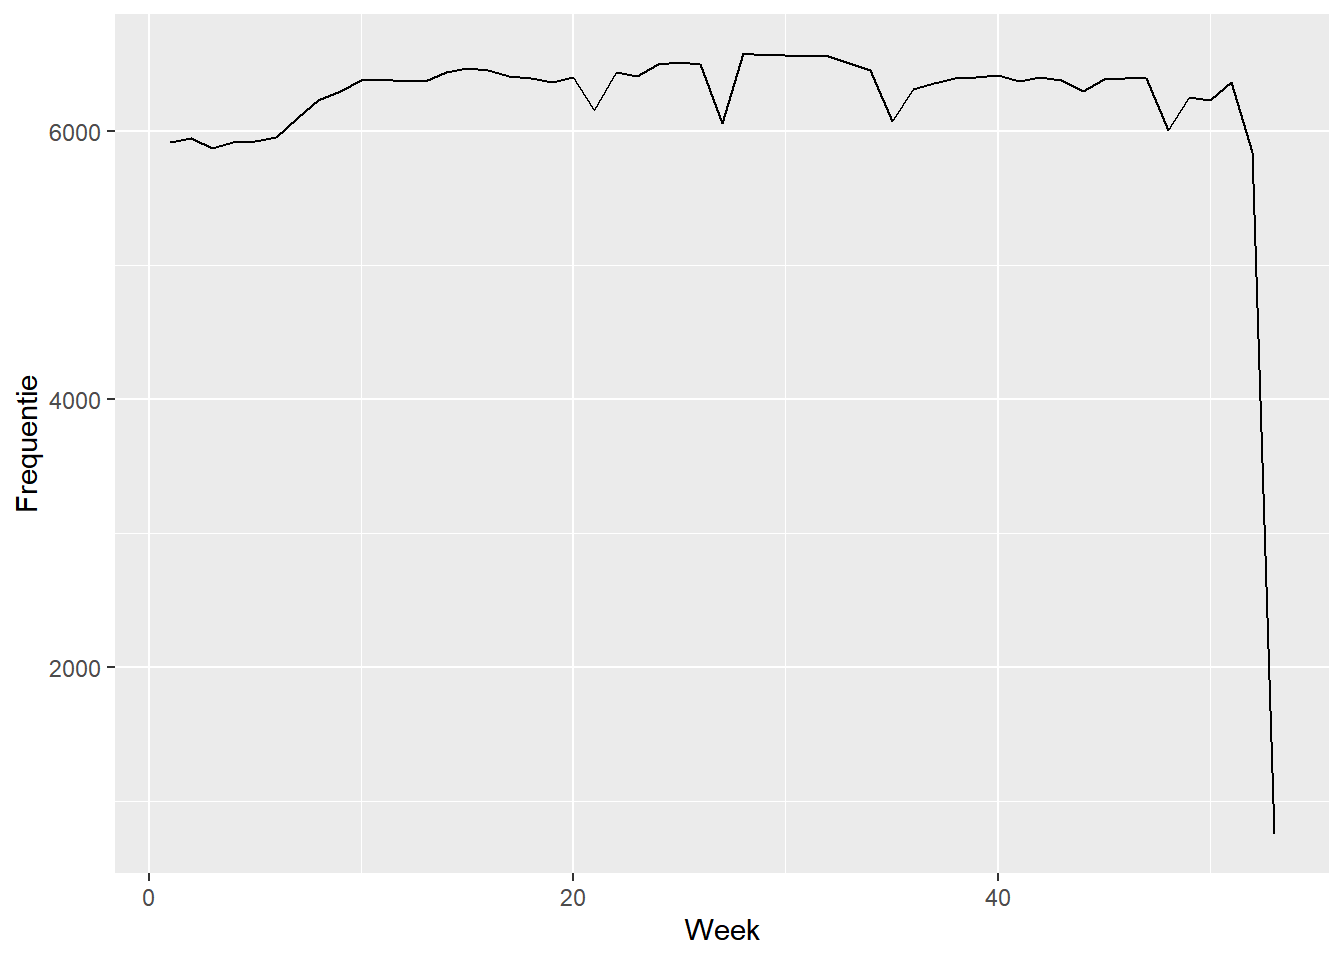
\includegraphics[width=0.49\linewidth]{lecture_notes_edda_files/figure-latex/2-15-1}

\hypertarget{datavisualisatie-met-meer-dan-2-variabelen}{%
\section{Datavisualisatie met meer dan 2 variabelen}\label{datavisualisatie-met-meer-dan-2-variabelen}}

\begin{itemize}
\tightlist
\item
  Datavisualisatie van patronen tussen meer dan 2 variabelen worden snel te complex om te interpreteren.
\item
  Het basisprincipe is wel eenvoudig.

  \begin{itemize}
  \tightlist
  \item
    Je hebt typisch 1 afhankelijke variabele (Y) en een aantal onafhankelijke variabelen (A, B, \ldots{}).
  \item
    De bedoeling is het effect van de onafhankelijke variabelen op de afhankelijke variabele te visualiseren.
  \item
    Hierbij definiëren we een orde tussen de onafhankelijke variabelen. We duiden de eerste-orde onafhankelijke variabele aan als A, de tweede-orde onafhankelijke variabele als B, enzovoort.
  \item
    De bedoeling is om in eerste instantie het patroon weer te geven tussen A en Y en vervolgens de invloed van B op dit patroon.
  \item
    Dit betekent dat je in eerste instantie een gewone bivariate plot tussen A en Y construeert en deze dan aanpast om de impact van B te visualiseren.
  \end{itemize}
\end{itemize}

\hypertarget{onafhankelijke-variabele-b-2de-orde-is-categorisch.}{%
\subsection{Onafhankelijke variabele B (2de orde) is categorisch.}\label{onafhankelijke-variabele-b-2de-orde-is-categorisch.}}

\begin{itemize}
\tightlist
\item
  Mogelijkheid 1 is per mogelijke waarde van variabele B een facet aan te maken.
\end{itemize}

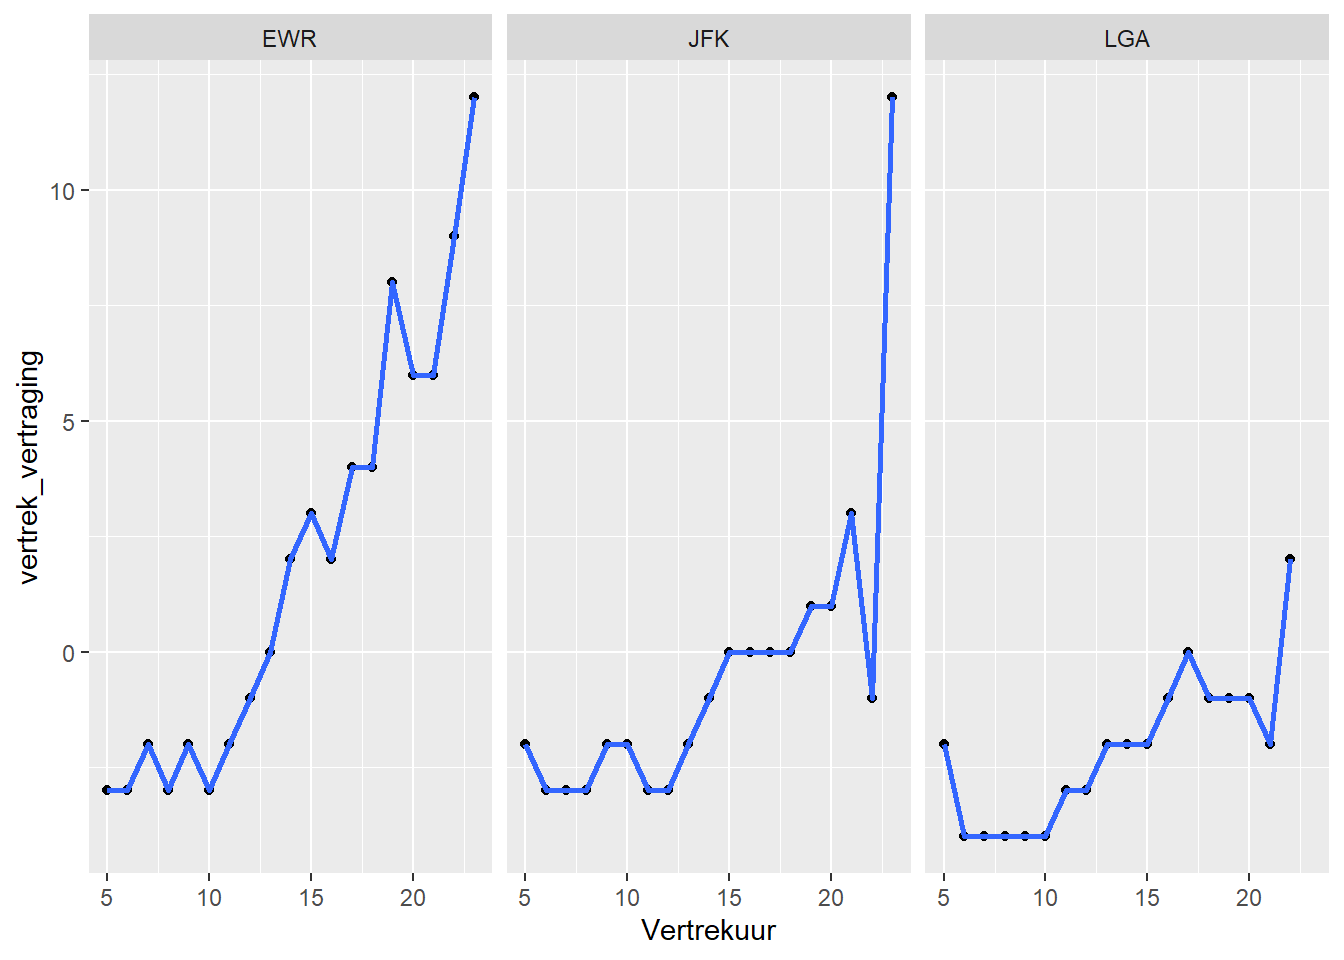
\includegraphics[width=0.49\linewidth]{lecture_notes_edda_files/figure-latex/2-16-1}

\begin{itemize}
\tightlist
\item
  Je kan dit principe ook toepassen als je nog een derde-orde onafhankelijke categorische variabele hebt.
\end{itemize}

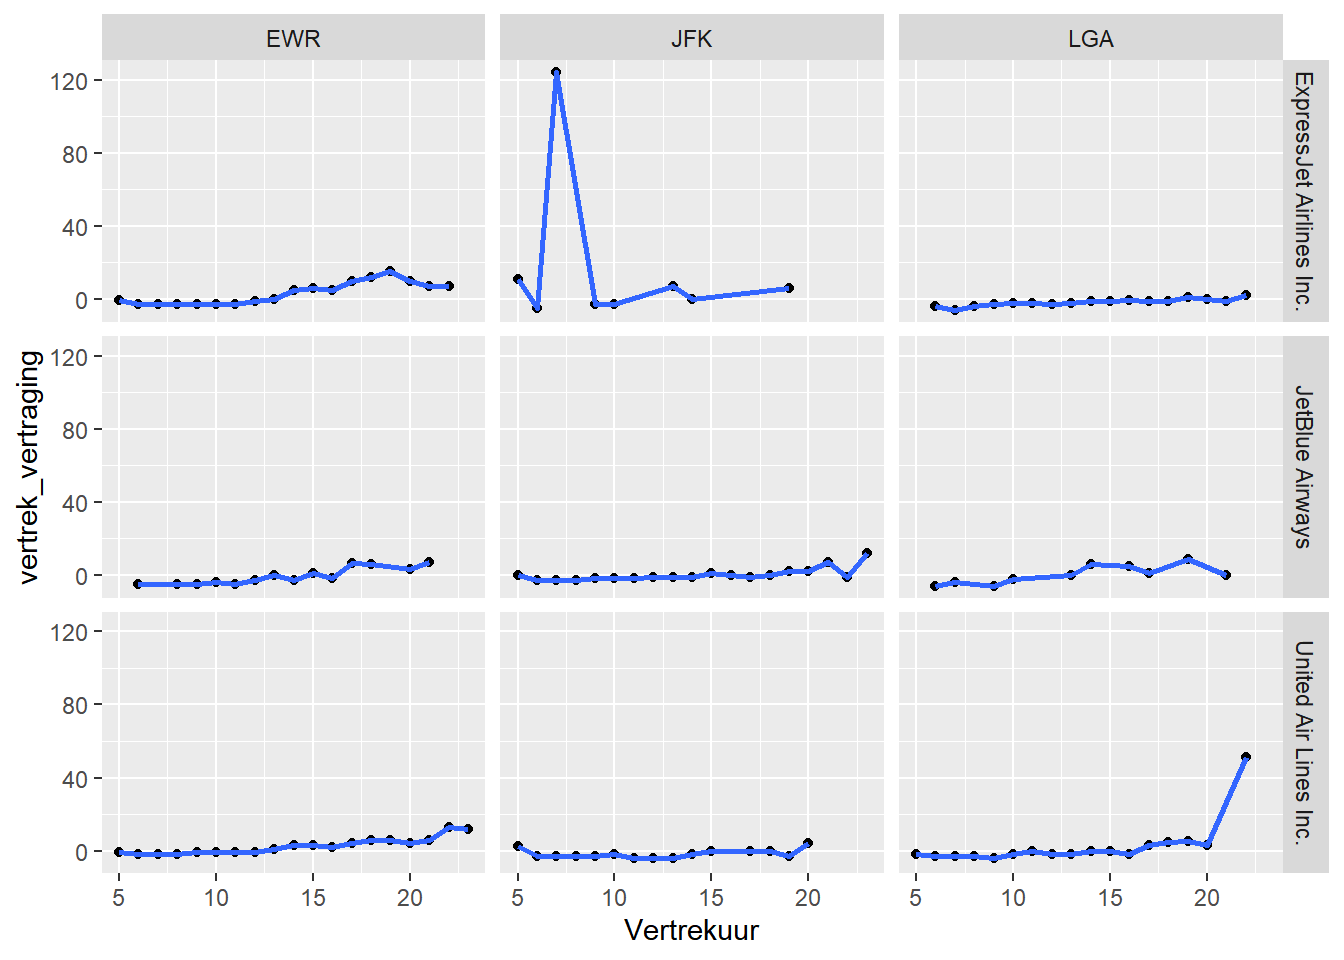
\includegraphics[width=0.49\linewidth]{lecture_notes_edda_files/figure-latex/2-17-1}

\begin{itemize}
\tightlist
\item
  Een tweede mogelijkheid is een ander aspect van de visualisatie aan de tweede onafhankelijke variabele B te koppelen. Bijvoorbeeld door een andere kleur te gebruiken voor verschillende waardes van variabele B.
\end{itemize}

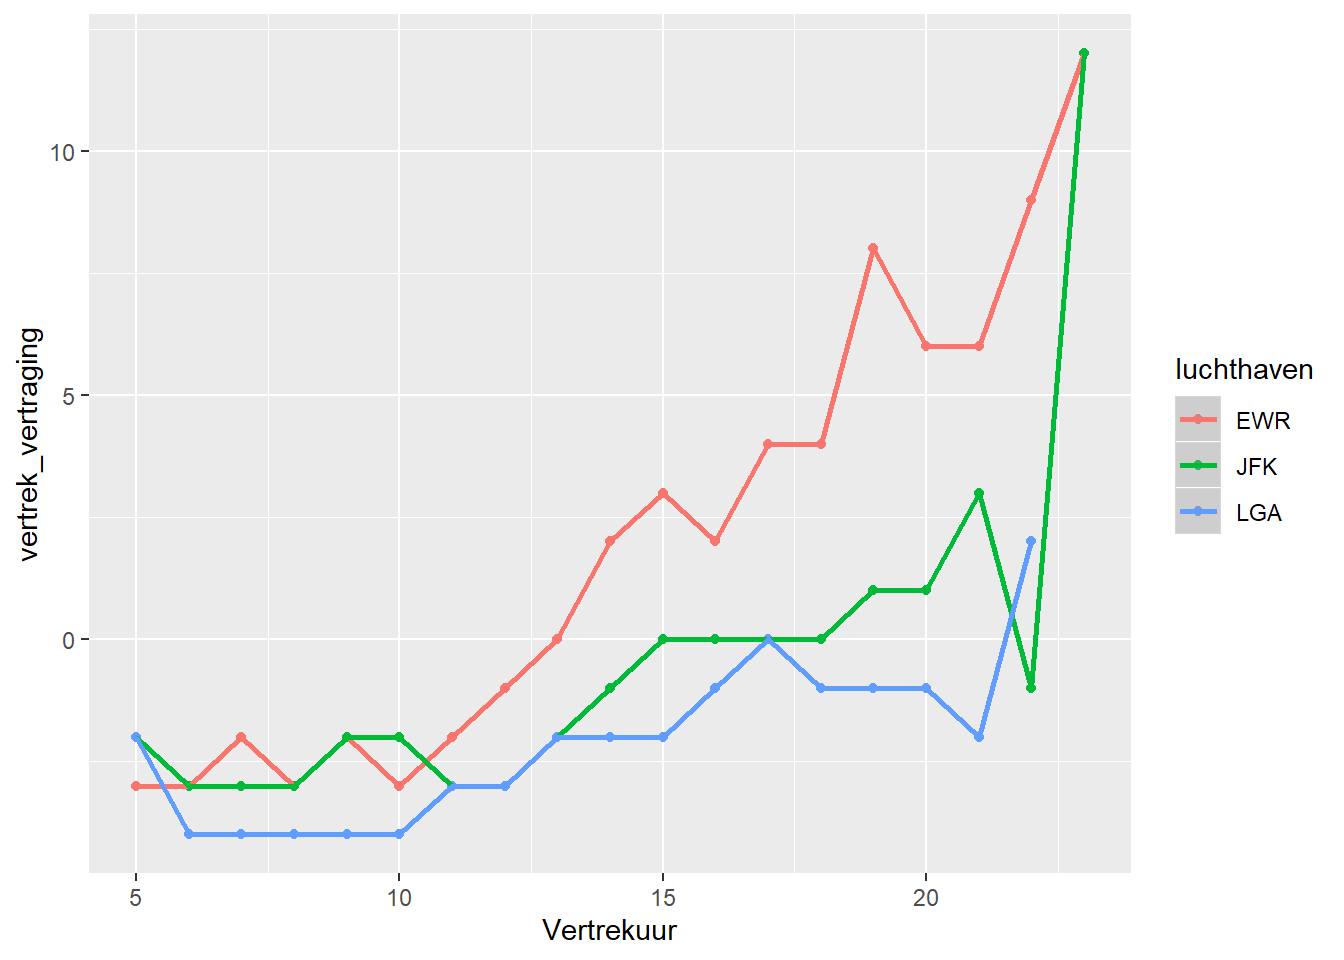
\includegraphics[width=0.49\linewidth]{lecture_notes_edda_files/figure-latex/2-18-1}

\hypertarget{referenties-1}{%
\section{Referenties}\label{referenties-1}}

\begin{enumerate}
\def\labelenumi{\arabic{enumi}.}
\tightlist
\item
  \href{http://www.mnestudies.com/research/scales-measurement}{Scales of Measurement}
\item
  \href{http://websites.uwlax.edu/tbrooks/eco307/handouts/velleman\%201993\%20-\%20typologies\%20misleading.pdf}{Nominal, Ordinal, Interval, and Ratio Typologies are Misleading}
\end{enumerate}

\hypertarget{beschrijvende-statistieken}{%
\chapter{Beschrijvende statistieken}\label{beschrijvende-statistieken}}

\hypertarget{beschrijvende-statistieken-versus-exploratieve-plots}{%
\section{Beschrijvende statistieken versus exploratieve plots}\label{beschrijvende-statistieken-versus-exploratieve-plots}}

\begin{itemize}
\tightlist
\item
  Plots zijn vooral sterk om patronen in de data te visualiseren.
\item
  Plots zijn minder geschikt om de `sterkte' of `grootte' van een patroon uit te drukken.
\item
  Beschrijvende statistieken laten dit wel toe aangezien aspecten van de patronen in een exploratieve plot in exacte getallen worden gegoten.
\item
  Er kunnen hoofdzakelijk 3 soorten beschrijvende statistieken worden onderscheiden:

  \begin{itemize}
  \tightlist
  \item
    Centrummaten
  \item
    Spreidingsmaten
  \item
    Associatiematen
  \end{itemize}
\item
  Centrummaten en spreidingsmaten zijn univariate statistieken en hebben als doel de verdeling van 1 variabele data samen te vatten in 2 cijfers.
\item
  Associatiematen zijn typisch bivariate statistieken en hebben als doel de samenhang tussen twee variabelen samen te vatten.
\end{itemize}

\hypertarget{notatie}{%
\section{Notatie}\label{notatie}}

\begin{itemize}
\tightlist
\item
  \(n\): aantal observaties.
\item
  \(X, Y\): variabelen.
\item
  \(x_i, y_i\): de waarden voor variabelen \(X\) en \(Y\) voor observatie \(i\).
\item
  \(x_{(i)}\): de \(i\)-de waarde voor \(X\) na rangschikking van klein naar groot.
\end{itemize}

\hypertarget{data-1}{%
\section{Data}\label{data-1}}

\begin{table}[t]

\caption{\label{tab:4-2b}Uitgaande vluchten NYC 2013}
\centering
\fontsize{10}{12}\selectfont
\begin{tabular}{lllrrrrl}
\toprule
luchthaven & maatschappij & datum & vertrek\_vertraging & aankomst\_vertraging & afstand & vliegtijd & vluchttype\\
\midrule
EWR & United Air Lines Inc. & 2013-01-01 05:15:00 & 2 & 11 & 1400 & 227 & normaal\\
LGA & United Air Lines Inc. & 2013-01-01 05:29:00 & 4 & 20 & 1416 & 227 & normaal\\
JFK & American Airlines Inc. & 2013-01-01 05:40:00 & 2 & 33 & 1089 & 160 & kort\\
LGA & Delta Air Lines Inc. & 2013-01-01 06:00:00 & -6 & -25 & 762 & 116 & kort\\
EWR & United Air Lines Inc. & 2013-01-01 05:58:00 & -4 & 12 & 719 & 150 & kort\\
\addlinespace
EWR & JetBlue Airways & 2013-01-01 06:00:00 & -5 & 19 & 1065 & 158 & kort\\
LGA & ExpressJet Airlines Inc. & 2013-01-01 06:00:00 & -3 & -14 & 229 & 53 & kort\\
JFK & JetBlue Airways & 2013-01-01 06:00:00 & -3 & -8 & 944 & 140 & kort\\
LGA & American Airlines Inc. & 2013-01-01 06:00:00 & -2 & 8 & 733 & 138 & kort\\
JFK & JetBlue Airways & 2013-01-01 06:00:00 & -2 & -2 & 1028 & 149 & kort\\
\bottomrule
\end{tabular}
\end{table}

\hypertarget{univariate-statistieken}{%
\section{Univariate statistieken}\label{univariate-statistieken}}

\hypertarget{categorische-variabele-1}{%
\subsection{Categorische variabele}\label{categorische-variabele-1}}

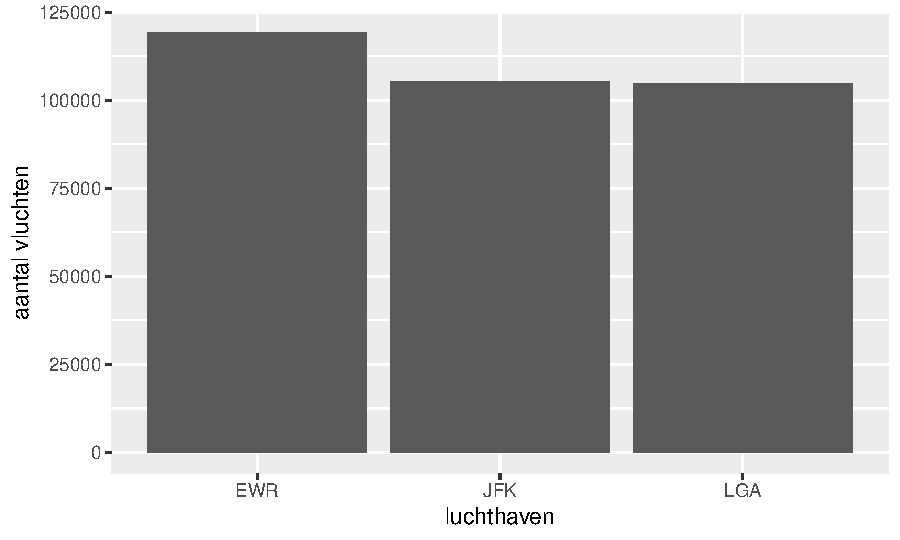
\includegraphics[width=0.49\linewidth]{lecture_notes_edda_files/figure-latex/4-3-1}
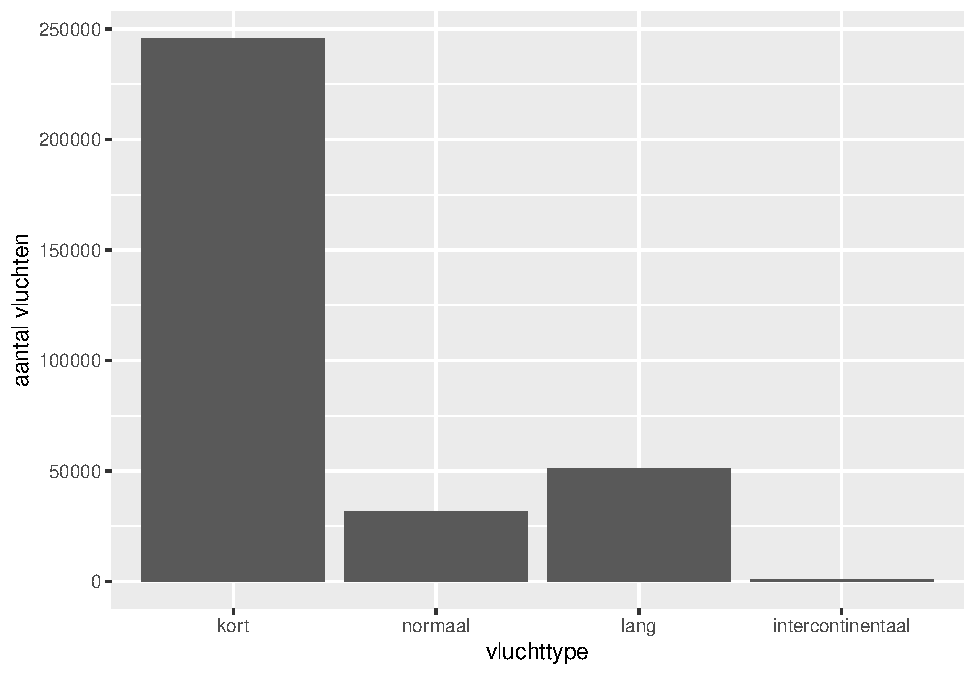
\includegraphics[width=0.49\linewidth]{lecture_notes_edda_files/figure-latex/4-3-2}

\hypertarget{frequentietabel}{%
\subsubsection*{Frequentietabel}\label{frequentietabel}}
\addcontentsline{toc}{subsubsection}{Frequentietabel}

\begin{itemize}
\tightlist
\item
  De absolute frequentie \(f\) geeft aan hoe vaak een waarde voorkomt.
\item
  De relatieve frequentie \(f/n\) geeft aan welk aandeel deze frequentie heeft in het totaal aantal elementen \(n\).
\item
  De cumulatieve frequentie \(F_n(x)\) van een bepaalde waarde \(x\) geeft aan hoeveel observaties kleiner zijn dan of gelijk zijn aan \(x\).
\item
  De cumulatieve relatieve frequentie \(F_n(x)/n\) van een bepaalde waarde \(x\) geeft aan hoeveel percent van de observaties kleiner zijn dan of gelijk zijn aan \(x\).
\item
  Een frequentietabel laat voor alle mogelijke waarden van een categorische variabele de absolute en relatieve frequentie zien (zowel normaal als cumulatief).
\item
  Een frequentietabel laat zien waar een bepaalde waarde zich precies in de verdeling bevindt en hoe uitzonderlijk het is een specifieke waarde in de data te zien (of een waarde groter/kleiner dan) .
\end{itemize}

\begin{table}[t]

\caption{\label{tab:4-4}Aantal vluchten per luchthaven}
\centering
\fontsize{10}{12}\selectfont
\begin{tabular}{lrrrr}
\toprule
luchthaven & freq & rel\_freq & cum\_freq & cum\_rel\_freq\\
\midrule
EWR & 119282 & 0.36 & 119282 & 0.36\\
JFK & 105230 & 0.32 & 224512 & 0.68\\
LGA & 104662 & 0.32 & 329174 & 1.00\\
\bottomrule
\end{tabular}
\end{table}

\hypertarget{centrummaten}{%
\subsubsection*{Centrummaten}\label{centrummaten}}
\addcontentsline{toc}{subsubsection}{Centrummaten}

\begin{itemize}
\tightlist
\item
  Modus

  \begin{itemize}
  \tightlist
  \item
    Meest voorkomende waarde.
  \item
    Enige centrummaat voor nominale variabele.
  \item
    Ook bruikbaar voor ordinale variabele.
  \item
    Een variabele kan meerdere modi hebben.
  \item
    De modus is robuust tegen uitschieters.
  \item
    De modus kan je aflezen als de eerste rij in een frequentietabel als je deze ordent van de meest voorkomende tot de minst voorkomende waarde.
  \end{itemize}
\item
  Mediaan

  \begin{itemize}
  \tightlist
  \item
    De middelste waarde na rangschikken van de gegevens.
  \item
    Voor ordinale variabelen definiëren we de mediaan aan de hand van de relatieve cumulatieve frequentie. De mediaan is de kleinste waarde waar 50\% van de observaties kleiner dan of gelijk aan is.
  \item
    De mediaan is robuust tegen uitschieters.
  \end{itemize}
\end{itemize}

\begin{table}[t]

\caption{\label{tab:4-5}Aantal vluchten per vluchttype}
\centering
\fontsize{10}{12}\selectfont
\begin{tabular}{lrrrr}
\toprule
vluchttype & freq & rel\_freq & cum\_freq & cum\_rel\_freq\\
\midrule
kort & 245666 & 0.75 & 245666 & 0.75\\
normaal & 31813 & 0.10 & 277479 & 0.85\\
lang & 50980 & 0.15 & 328459 & 1.00\\
intercontinentaal & 715 & 0.00 & 329174 & 1.00\\
\bottomrule
\end{tabular}
\end{table}
\begin{table}[t]

\caption{\label{tab:4-6}Centrummaten voor vluchttype}
\centering
\fontsize{10}{12}\selectfont
\begin{tabular}{ll}
\toprule
variabele & mediaan\\
\midrule
vluchttype & kort\\
\bottomrule
\end{tabular}
\end{table}

\hypertarget{spreidingsmaten}{%
\subsubsection*{Spreidingsmaten}\label{spreidingsmaten}}
\addcontentsline{toc}{subsubsection}{Spreidingsmaten}

\begin{itemize}
\tightlist
\item
  Kwantielen.

  \begin{itemize}
  \tightlist
  \item
    Kwantielen (of percentielen) zijn gebaseerd op de cumulatieve relatieve frequentie.
  \item
    Het p\% kwantiel is de kleinste waarde waar p\% van de observaties kleiner dan of gelijk aan is.
  \item
    Het 50\% kwantiel komt overeen met de mediaan.
  \item
    Veel voorkomende kwantielen om de spreiding van de data weer te geven zijn het 25\% en 75\% kwantiel.
  \end{itemize}
\end{itemize}

\begin{table}[t]

\caption{\label{tab:4-7}Kwantielen voor vluchttype}
\centering
\fontsize{10}{12}\selectfont
\begin{tabular}{llll}
\toprule
variabele & Q25 & Q50 & Q75\\
\midrule
vluchttype & kort & kort & normaal\\
\bottomrule
\end{tabular}
\end{table}

\hypertarget{continue-variabele-1}{%
\subsection{Continue variabele}\label{continue-variabele-1}}

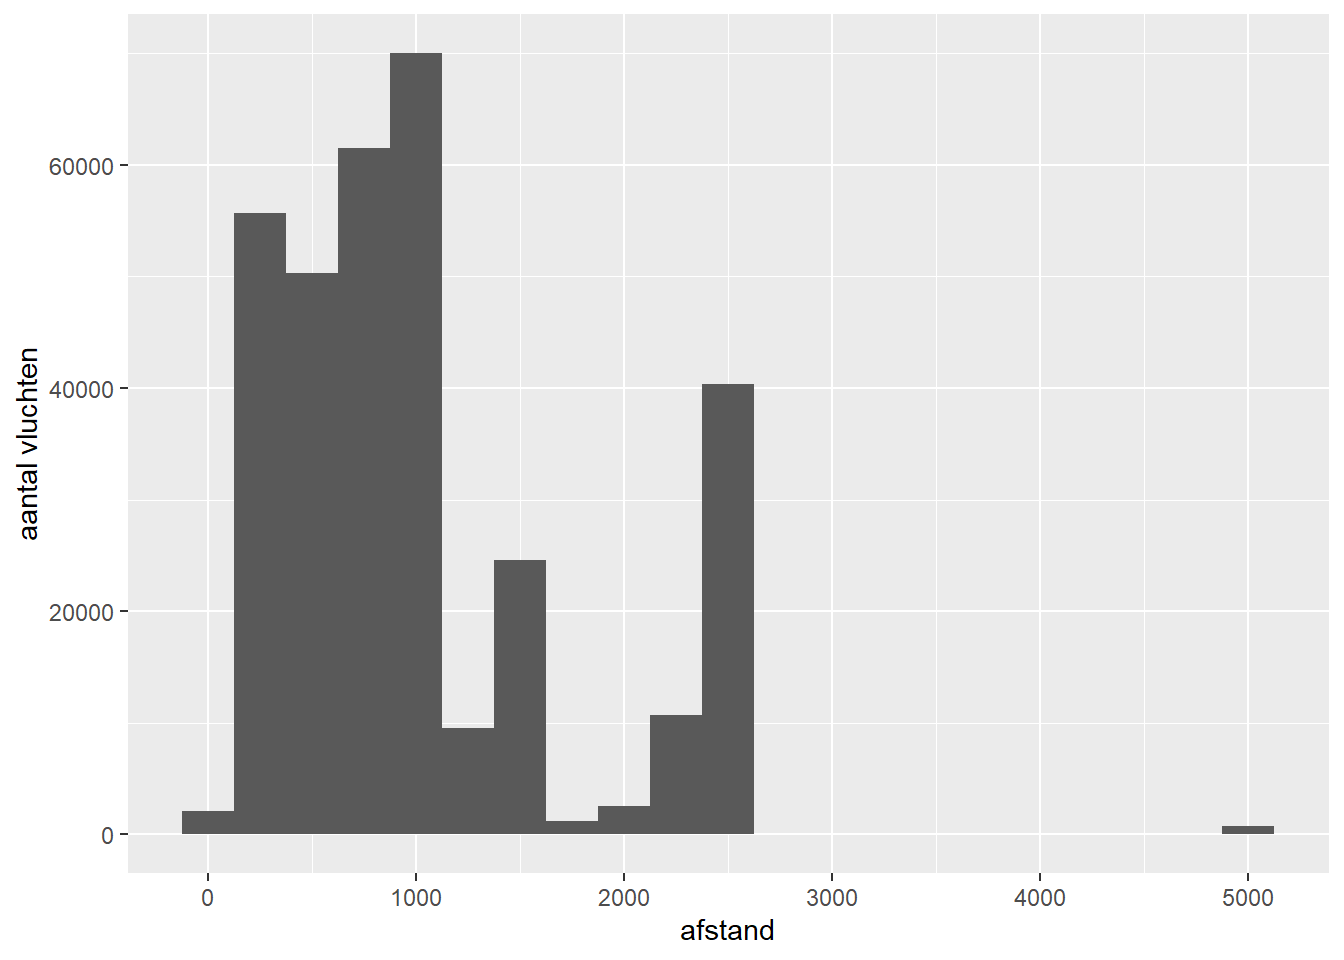
\includegraphics[width=0.49\linewidth]{lecture_notes_edda_files/figure-latex/4-8-1}

\hypertarget{centrummaten-1}{%
\subsubsection*{Centrummaten}\label{centrummaten-1}}
\addcontentsline{toc}{subsubsection}{Centrummaten}

\begin{itemize}
\tightlist
\item
  Modus

  \begin{itemize}
  \tightlist
  \item
    Vaak minder bruikbaar bij een continue variabelen omdat iedere waarde zeer weinig voorkomt. Bijgevolg zijn er vaak zeer veel modi met telkens slechts enkele observaties.
  \end{itemize}
\item
  Mediaan

  \begin{itemize}
  \tightlist
  \item
    De middelste waarde na rangschikking van de gegevens.
  \item
    In geval van een oneven aantal observaties, komt dit overeen met \(x_{\frac{(n+1)}{2}}\).
  \item
    In geval van een even aantal observaties zijn er twee `middelste' observaties en is de mediaan gelijk aan \(\frac{1}{2}( x_{\frac{n}{2}}+x_{\frac{n}{2}+1})\)
  \item
    De mediaan is robuust tegen uitschieters.
  \end{itemize}
\item
  (Rekenkundig) Gemiddelde

  \begin{itemize}
  \tightlist
  \item
    \(\bar{x} = \frac{1}{n}\sum_{i=1}^n x_i\)
  \item
    Het gemiddelde is gevoelig voor uitschieters.
  \item
    Dit is de centrummaat die mensen intuïtief selecteren indien mogelijk.
  \end{itemize}
\end{itemize}

\begin{table}[t]

\caption{\label{tab:4-9}Afstand (centrummaten)}
\centering
\fontsize{10}{12}\selectfont
\begin{tabular}{lrr}
\toprule
variabele & gemiddelde & mediaan\\
\midrule
afstand & 1026.98 & 820\\
\bottomrule
\end{tabular}
\end{table}

\hypertarget{spreidingsmaten-1}{%
\subsubsection*{Spreidingsmaten}\label{spreidingsmaten-1}}
\addcontentsline{toc}{subsubsection}{Spreidingsmaten}

\begin{itemize}
\tightlist
\item
  Kwantielen
\item
  Bereik

  \begin{itemize}
  \tightlist
  \item
    Dit is het verschil tussen de grootste en kleinste waarde.
  \item
    Zeer gevoelig voor uitschieters.
  \item
    Is slechts gebaseerd op 2 observaties en bevat dus weinig informatie. Hiermee bedoelen we dat de spreiding van 2 variabelen sterk kan verschillen terwijl ze toch hetzelfde bereik hebben.
  \end{itemize}
\item
  Interkwartielafstand (IQR)

  \begin{itemize}
  \tightlist
  \item
    Dit is het verschil tussen Q75 en Q25.
  \item
    Zelfde principe als het bereik, maar minder gevoelig voor uitschieters.
  \item
    IQR is ook slechts gebaseerd op 2 observaties.
  \end{itemize}
\item
  Gemiddelde absolute afwijking (average absolute deviation)

  \begin{itemize}
  \tightlist
  \item
    Dit is de gemiddelde afwijking ten opzichte van het gemiddelde over alle observaties.
  \item
    \(\frac{1}{n}\sum_{i=1}^{n}\lvert x_i - \bar{x} \rvert\).
  \end{itemize}
\item
  Variantie

  \begin{itemize}
  \tightlist
  \item
    \(s^2 = \frac{1}{n-1}\sum_{i=1}^{n}(x_i - \bar{x})^2\).
  \item
    Vergelijkbaar met gemiddelde absolute afwijking, maar nu wordt het kwadraat gebruikt om te voorkomen dat de verschillen ten opzichte van het gemiddelde elkaar opheffen.
  \item
    Vanuit analytisch standpunt is deze spreidingsmaat interessanter (geen absolute waardes, waardoor afgeleiden bijvoorbeeld eenvoudiger worden om te berekenen).
  \item
    Wel gevoelig voor uitschieters en door het kwadraat wordt het effect van deze uitschieters ook nog eens vergroot.
  \item
    De wortel van de variantie wordt de standaardafwijking genoemd. De standaardafwijking heeft het voordeel dat het indezelfde eenheid uitgedrukt wordt als de oorspronkelijke data.
  \end{itemize}
\item
  Median Absolute Deviation (MAD)

  \begin{itemize}
  \tightlist
  \item
    Dit is de middelste afwijking ten opzichte van de mediaan over alle observaties.
  \item
    \(\operatorname{MAD} = \operatorname{median}\left(\ \left| X_{i} - \operatorname{median} (X) \right|\ \right)\).
  \item
    Deze maatstaf is robuster tegen outliers.
  \end{itemize}
\end{itemize}

\begin{table}[t]

\caption{\label{tab:4-10}Afstand (spreidingsmaten)}
\centering
\resizebox{\linewidth}{!}{
\fontsize{10}{12}\selectfont
\begin{tabular}{lrrrrrrrrr}
\toprule
variabele & minimum & Q25 & Q50 & Q75 & maximum & bereik & IQR & var & sd\\
\midrule
afstand & 17 & 502 & 820 & 1372 & 4983 & 4966 & 870 & 542630.2 & 736.6344\\
\bottomrule
\end{tabular}}
\end{table}

\hypertarget{bivariate-statistieken}{%
\section{Bivariate statistieken}\label{bivariate-statistieken}}

\hypertarget{continu-versus-continu}{%
\subsection{Continu versus Continu}\label{continu-versus-continu}}

\begin{verbatim}
## `geom_smooth()` using method = 'gam' and formula 'y ~ s(x, bs = "cs")'
\end{verbatim}

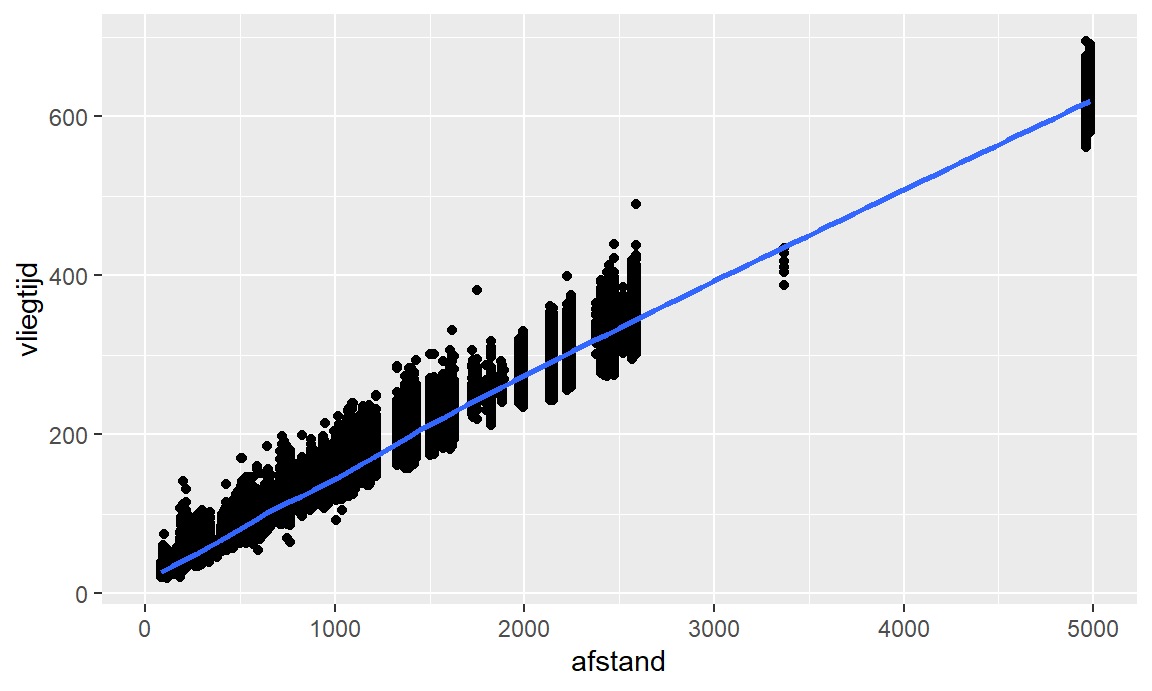
\includegraphics[width=0.49\linewidth]{lecture_notes_edda_files/figure-latex/4-11-1}

\hypertarget{correlatie}{%
\subsubsection*{Correlatie}\label{correlatie}}
\addcontentsline{toc}{subsubsection}{Correlatie}

\begin{itemize}
\tightlist
\item
  Covariantie

  \begin{itemize}
  \tightlist
  \item
    \(cov(x,y) = \frac{1}{n-1}\sum_{i=1}^{n}(x_i - \bar(x))(y_i-\bar(y))\).
  \item
    Bij een positieve associatie tussen twee variabelen zal de covariantie positief zijn.
  \item
    Bij een negatieve associatie tussen twee variabelen zal de covariantie negatief zijn.
  \item
    De covariantie is echter afhankelijk van de maateenheid van de variabelen, waardoor ze weinig bruikbaar is om de sterkte van de associatie weer te geven.
  \end{itemize}
\item
  Pearson correlatiecoëfficiënt

  \begin{itemize}
  \tightlist
  \item
    Herschaalt de covariantie naar de schaal \([-1,1]\)
  \item
    Laat toe om de sterkte van een associatie te evalueren.
  \item
    \(r(x,y) = \frac{cov(x,y)}{s_x s_y}\)
  \item
    \(r(x,y) = \frac{\sum_{i=1}^{n}(x_i-\bar{x})(y_i-\bar{y})}{\sqrt{\sum_{i=1}^{n}(x_i-\bar{x})^2 \sum_{i=1}^{n}(y_i-\bar{y})^2}}\)
  \item
    Meet \textbf{lineaire} associatie tussen 2 variabelen.
  \item
    Twee variabelen kunnen positief geassocieerd zijn, maar in een niet-lineaire wijze, waardoor de correlatiecoëfficiënt naar nul gaat.
  \item
    Meest gebruikelijke correlatiecoëfficiënt voor continue variabelen.
  \item
    Daarom best altijd samen met een puntenwolk bekijken.
  \end{itemize}
\item
  Spearman's rangcorrelatiecoëfficiënt.

  \begin{itemize}
  \tightlist
  \item
    Zelfde principe als Pearson's, maar dan gebaseerd op de rangorde van de waarden in plaats van de waarden zelf.
  \item
    \(r_i\): rangorde van waarde \(x_i\). Bijvoorbeeld \(r_i = 4\) betekent dat de waarde \(x_i\) de vierde kleinste waarde is.
  \item
    \(s_i\): rangorde van waarde \(y_i\).
  \item
    \(\rho(x,y) = \frac{\sum_{i=1}^{n}(r_i-\bar{r})(s_i-\bar{s})}{\sqrt{\sum_{i=1}^{n}(r_i-\bar{r})^2 \sum_{i=1}^{n}(s_i-\bar{s})^2}}\)
  \item
    Meet associatie tussen 2 variabelen, dus niet specifiek lineaire associatie.
  \end{itemize}
\item
  Kendall's correlatiecoëfficiënt

  \begin{itemize}
  \tightlist
  \item
    Ook wel Kendall's tau genoemd.
  \item
    De methode is gebaseerd door alle mogelijke observatieparen \((x_i, y_i)\) en \((x_j,y_j)\) te bestuderen.
  \item
    Net als Spearman's aanpak gebaseerd op rangorde \((r_i, s_i)\) en niet de feitelijke waarden.
  \item
    Indien \(r_i > r_j\) en \(s_i > s_j\) (of \(r_i < r_j\) en \(s_i < s_j\)) dan zijn observaties \(i\) en \(j\) concordant.
  \item
    Indien \(r_i > r_j\) en \(s_i < s_j\) (of \(r_i < r_j\) en \(s_i > s_j\)) dan zijn observaties \(i\) en \(j\) discordant.
  \item
    Notatie: \(C\) en \(D\) zijn respectievelijk het aantal concordante en discordante paren.
  \item
    \(\tau = \frac{C-D}{\frac{1}{2}n(n-1)}\)
  \item
    Net als Spearman's correlatiecoëfficiënt, focust Kendall's tau op de associatie (positief of negatief) en niet specifiek op lineaire associatie.
  \item
    Het nadeel van Kendall's tau is dat je alle observatieparen moet bestuderen en het aantal kan snel exploderen bij veel observaties. Immers het aantal paren is \(\frac{n!}{2!(n-2)!}\). Hierdoor kan je Kendall in de praktijk niet gebruiken als je veel observaties hebt.
  \end{itemize}
\end{itemize}

\begin{table}[t]

\caption{\label{tab:4-12}Correlatie tussen afstand en vliegtijd}
\centering
\fontsize{10}{12}\selectfont
\begin{tabular}{lrr}
\toprule
variabelenpaar & pearson & spearman\\
\midrule
afstand-vliegtijd & 0.99 & 0.98\\
\bottomrule
\end{tabular}
\end{table}

\hypertarget{vergelijking-correlatiecoefficienten}{%
\subsubsection*{Vergelijking correlatiecoëfficiënten}\label{vergelijking-correlatiecoefficienten}}
\addcontentsline{toc}{subsubsection}{Vergelijking correlatiecoëfficiënten}

\begin{itemize}
\tightlist
\item
  Rangcorrelatiecoëfficiënten meten associatie, terwijl Pearson correlatiecoëfficiënt \textbf{lineaire} associatie meet!
\end{itemize}

\begin{table}[t]

\caption{\label{tab:4-13}Fictieve dataset}
\centering
\fontsize{10}{12}\selectfont
\begin{tabular}{rr}
\toprule
x & y\\
\midrule
1 & 0.0\\
2 & 4.0\\
3 & 5.0\\
4 & 5.5\\
5 & 7.0\\
\addlinespace
6 & 15.0\\
7 & 15.6\\
8 & 16.0\\
9 & 50.0\\
10 & 1000.0\\
\bottomrule
\end{tabular}
\end{table}

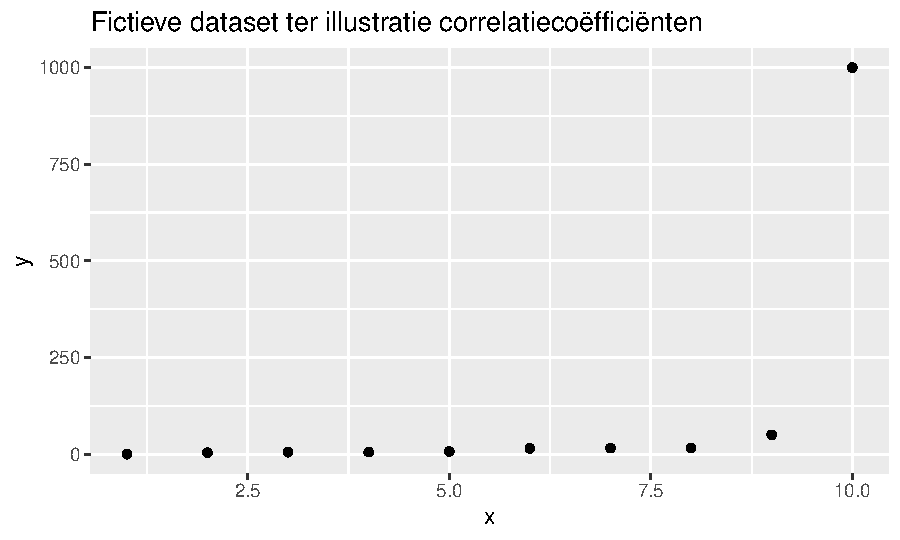
\includegraphics[width=0.49\linewidth]{lecture_notes_edda_files/figure-latex/4-14-1}

\begin{table}[t]

\caption{\label{tab:4-15}Correlatiecoëfficiënten fictieve dataset}
\centering
\fontsize{10}{12}\selectfont
\begin{tabular}{lrrr}
\toprule
variabelenpaar & pearson & spearman & kendall\\
\midrule
x-y & 0.55 & 1 & 1\\
\bottomrule
\end{tabular}
\end{table}

\hypertarget{categorisch-versus-continu}{%
\subsection{Categorisch versus Continu}\label{categorisch-versus-continu}}

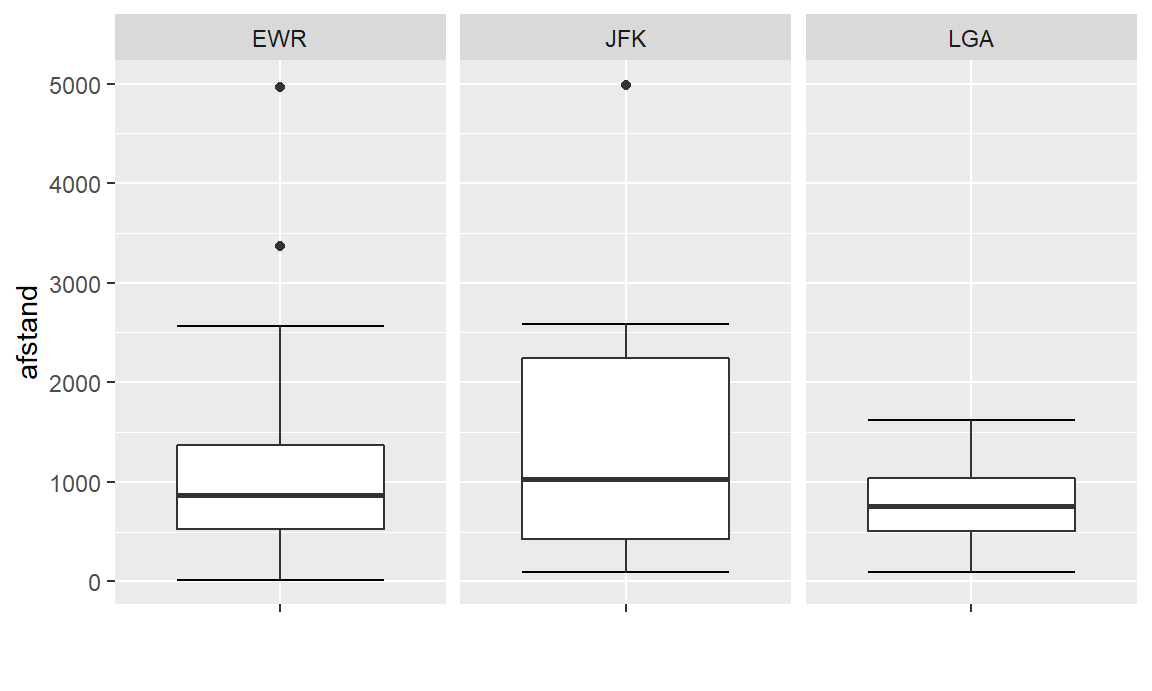
\includegraphics[width=0.49\linewidth]{lecture_notes_edda_files/figure-latex/4-16-1}

\hypertarget{univariate-statistieken-per-categoriewaarde}{%
\subsubsection*{Univariate statistieken per categoriewaarde}\label{univariate-statistieken-per-categoriewaarde}}
\addcontentsline{toc}{subsubsection}{Univariate statistieken per categoriewaarde}

\begin{itemize}
\tightlist
\item
  Je toont de relevante centrum- en spreidingsmaten voor de afhankelijke categorische variabele per waarde van de onafhankelijke categorische variabele.
\end{itemize}

\begin{table}[t]

\caption{\label{tab:4-17}Afstand-Luchthaven (centrummaten)}
\centering
\fontsize{10}{12}\selectfont
\begin{tabular}{lrr}
\toprule
luchthaven & gemiddelde & mediaan\\
\midrule
EWR & 1049.58 & 872\\
JFK & 1247.16 & 1028\\
LGA & 779.84 & 762\\
\bottomrule
\end{tabular}
\end{table}

\begin{table}[t]

\caption{\label{tab:4-18}Afstand-Luchthaven (spreidingsmaten)}
\centering
\resizebox{\linewidth}{!}{
\fontsize{10}{12}\selectfont
\begin{tabular}{lrrrrrrrrr}
\toprule
luchthaven & var & min & Q25 & Q50 & Q75 & max & bereik & IQR & sd\\
\midrule
EWR & 536177.0 & 17 & 529 & 872 & 1372 & 4963 & 4946 & 843 & 732.2411\\
JFK & 842460.4 & 94 & 425 & 1028 & 2248 & 4983 & 4889 & 1823 & 917.8564\\
LGA & 138132.3 & 96 & 502 & 762 & 1035 & 1620 & 1524 & 533 & 371.6615\\
\bottomrule
\end{tabular}}
\end{table}

\hypertarget{correlatie-1}{%
\subsubsection*{Correlatie}\label{correlatie-1}}
\addcontentsline{toc}{subsubsection}{Correlatie}

\begin{itemize}
\tightlist
\item
  Enkel toepasbaar als de categorische variabele ordinaal is.
\item
  Pearson's correlatiecoëfficiënt kan je NIET toepassen.
\item
  Spearman rangcorrelatiecoëfficiënt (\(\rho\)).
\item
  Kendall's rangcorrelatiecoëfficiënt (\(\tau\)) kan theoretisch wel toegepast worden, maar is in de praktijk vaak niet haalbaar.
\end{itemize}

\begin{table}[t]

\caption{\label{tab:unnamed-chunk-1}Correlatie tussen vluchttype en vliegtijd}
\centering
\fontsize{10}{12}\selectfont
\begin{tabular}{lr}
\toprule
variabelenpaar & spearman\\
\midrule
vluchttype-vliegtijd & 0.76\\
\bottomrule
\end{tabular}
\end{table}

\hypertarget{categorisch-versus-categorisch}{%
\subsection{Categorisch versus Categorisch}\label{categorisch-versus-categorisch}}

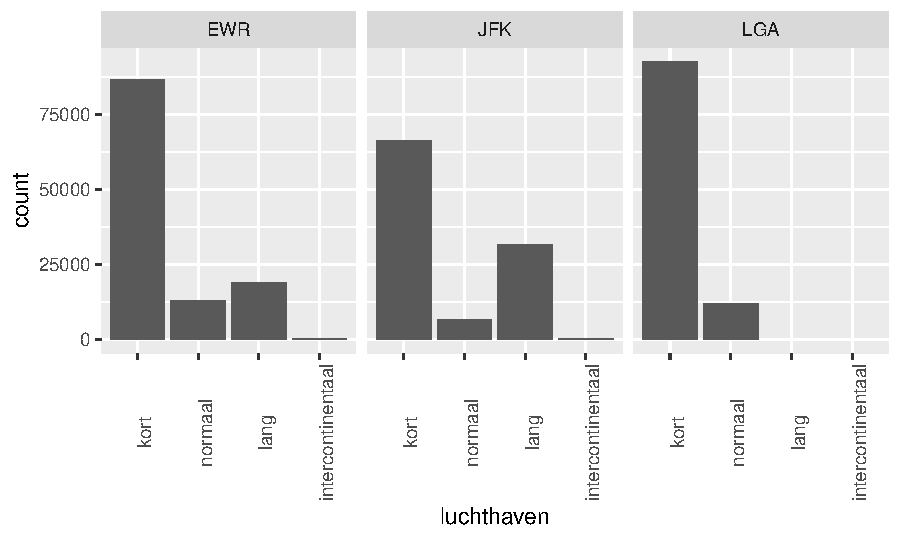
\includegraphics[width=0.49\linewidth]{lecture_notes_edda_files/figure-latex/4-20-1}

\hypertarget{univariate-statistieken-per-categoriewaarde-1}{%
\subsubsection*{Univariate statistieken per categoriewaarde}\label{univariate-statistieken-per-categoriewaarde-1}}
\addcontentsline{toc}{subsubsection}{Univariate statistieken per categoriewaarde}

\begin{itemize}
\tightlist
\item
  Je toont de relevante centrum- en spreidingsmaten voor de afhankelijke continue variabele per waarde van de onafhankelijke categorische variabele.
\end{itemize}

\begin{table}[t]

\caption{\label{tab:unnamed-chunk-2}Centrummaten voor vluchttype-luchthaven}
\centering
\fontsize{10}{12}\selectfont
\begin{tabular}{lll}
\toprule
luchthaven & variabele & mediaan\\
\midrule
EWR & vluchttype & kort\\
JFK & vluchttype & kort\\
LGA & vluchttype & kort\\
\bottomrule
\end{tabular}
\end{table}

\begin{table}[t]

\caption{\label{tab:unnamed-chunk-3}Kwantielen voor vluchttype-luchthaven}
\centering
\fontsize{10}{12}\selectfont
\begin{tabular}{lllll}
\toprule
luchthaven & variabele & Q25 & Q50 & Q75\\
\midrule
EWR & vluchttype & kort & kort & normaal\\
JFK & vluchttype & kort & kort & lang\\
LGA & vluchttype & kort & kort & kort\\
\bottomrule
\end{tabular}
\end{table}

\hypertarget{referenties-2}{%
\section*{Referenties}\label{referenties-2}}
\addcontentsline{toc}{section}{Referenties}

\begin{enumerate}
\def\labelenumi{\arabic{enumi}.}
\tightlist
\item
  Tekst Beleidsstatistiek: Hoofdstukken 1 en 2 en secties 4.2 en 4.3 (Blackboard)
\item
  \href{https://nl.wikipedia.org/wiki/Spearmans_rangcorrelatieco\%C3\%ABffici\%C3\%ABnt}{Spearman's rangcorrelatiecoëfficiënt}
\item
  \href{https://nl.wikipedia.org/wiki/Kendalls_tau}{Kendall's rangcorrelatiecoëfficiënt}
\item
  \href{https://www.researchgate.net/post/Does_Spearmans_rho_have_any_advantage_over_Kendalls_tau}{Spearman versus Kendall's correlatiecoëfficiënt}
\end{enumerate}

\hypertarget{exploratief-data-analyse-proces}{%
\chapter{Exploratief Data Analyse Proces}\label{exploratief-data-analyse-proces}}

Voor dit topic zijn er geen aparte lecture nodes, maar wordt verwezen naar de eerste 4 hoofdstukken in ``The Art of Data Science'' van Roger Peng en Elizabeth Matsui (tot en met hoofdstuk `Exploratory Data Analysis'). Dit boek kan men gratis bekomen via volgende link: \url{https://leanpub.com/artofdatascience} .

Let op: Boven aan de pagina wordt het boek + video lectures aangeboden voor een minimum prijs van 20 dollar. Maar als je naar onder scrolt vind je ook een link naar enkel het boek waarvoor de minimumprijs 0 dollar is. Als je hier op klikt kan je vervolgens zelf je prijs bepalen (en dus ook op 0 dollar zetten) om vervolgens het boek gratis aan te schaffen.

\hypertarget{datavoorbereiding}{%
\chapter{Datavoorbereiding}\label{datavoorbereiding}}

\hypertarget{beginnen-bij-het-begin}{%
\section{Beginnen bij het begin}\label{beginnen-bij-het-begin}}

\begin{itemize}
\tightlist
\item
  Alvorens we aan een exploratieve data analyse kunnen beginnen, moeten we eerst onze data voorbereiden.
\item
  Er kunnen drie grote fases geïdentificeerd worden tijdens de datavoorbereiding.

  \begin{itemize}
  \tightlist
  \item
    Correct inlezen van de data.
  \item
    Identificeren van problemen in de data en deze corrigeren van de data.
  \item
    Opwaarderen van de data.
  \end{itemize}
\item
  Data kan in diverse formaten aangeleverd worden en de eerste stap is ervoor zorgen dat de data ingeladen is in R. Hierbij zijn er twee specifieke elementen om aandacht aan te schenken:

  \begin{itemize}
  \tightlist
  \item
    De data analist moet ervoor zorgen dat de data correct ingeladen wordt en dat de inhoud na het inladen overeenkomt met de inhoud toen deze data de laatste keer werd opgeslagen.
  \item
    De data analist moet ervoor zorgen dat de verschillende variabelen het juiste data type hebben.
  \end{itemize}
\item
  De volgende fase is het opkuisen van de data. Dit betekent dat men fouten gaat identificeren en deze `oplost' alvorens verder te gaan.

  \begin{itemize}
  \tightlist
  \item
    Er zijn verschillende soorten fouten die in de data kunnen sluipen. Enkele mogelijke fouten zijn:

    \begin{itemize}
    \tightlist
    \item
      Sommige waarden ontbreken (geen waarde voor bepaalde variabele bij bepaalde observaties).
    \item
      Sommige waarden zijn fout. Bijvoorbeeld: voor een deel observaties is de afstand in km opgeslagen ipv mijl of is er een typfout in de waarde van een categorische variabele.
    \item
      Sommige observaties staan meerdere keren in de dataset.
    \end{itemize}
  \item
    Het opkuisen van data gebeurt in principe in 2 stappen:

    \begin{itemize}
    \tightlist
    \item
      Eerst moeten we de data bestuderen en fouten identificeren.
    \item
      Vervolgens moeten we de fouten in de data `corrigeren' (indien mogelijk).
    \end{itemize}
  \end{itemize}
\item
  Het opwaarderen van de data betreft een reeks transformaties met als doel de data bruikbaarder te maken voor exploratieve data analyse. Er zijn verschillende manieren om dit te bereiken:

  \begin{itemize}
  \tightlist
  \item
    Bestaande variabelen transformeren naar nieuwe variabelen die geschikter zijn om patronen in de data bloot te leggen. Bijvoorbeeld het transformeren van een continue variabele naar een categorische variabele of het creëren van een nieuwe variabele `gemiddelde snelheid' op basis van de variabelen `reistijd' en `totaal afgelegde afstand'.
  \item
    Het opsplitsen van de dataset in meerdere datasets die apart bestudeerd worden. Dit is vooral zinvol indien de dataset verschillende soorten observaties bevat of een deel observaties met uitzonderlijke waarden.
  \end{itemize}
\end{itemize}

\hypertarget{data-inlezen}{%
\section{Data inlezen}\label{data-inlezen}}

\hypertarget{uitdagingen-bij-het-correct-inlezen-van-data}{%
\subsection{Uitdagingen bij het correct inlezen van data}\label{uitdagingen-bij-het-correct-inlezen-van-data}}

\begin{itemize}
\tightlist
\item
  Data kan in verschillende formaten aangeleverd worden. Afhankelijk van het formaat, zal je andere functies moeten gebruiken om de data correct in te lezen
\item
  Maar zelfs als je de juiste functie gebruikt, kan het inlezen fout gaan omdat een computer data altijd als een reeks van 1 en 0'en opslaat en er daarom een soort vertaalsleutel nodig is van 1 en 0'en naar leesbare tekst. Deze vertaalslag wordt gerealiseerd door encoderingschema's en je moet er voor zorgen dat bij het inlezen van data je het juiste encoderingschema hanteert.
\item
  Eenmaal de data is ingeladen, moet je er voor zorgen dat R de datatypes juist identificeert. De meeste dataformaten houden geen informatie bij van welk datatype een specifieke variabele is en dus moet R dit `raden'. Omdat dit wel eens fout kan gaan, moet je als analist dit controleren en corrigeren waar nodig.
\end{itemize}

\hypertarget{dataformaten}{%
\subsection{Dataformaten}\label{dataformaten}}

\hypertarget{flat-file-databestanden}{%
\subsubsection{Flat-file databestanden}\label{flat-file-databestanden}}

\begin{itemize}
\tightlist
\item
  Lees de bron over \href{https://www.techwalla.com/articles/what-is-a-delimited-a-fixed-width-file}{delimited en fixed-width bestanden}.
\item
  Flat-file databestanden bevatten data die in een tabelvorm passen:

  \begin{itemize}
  \tightlist
  \item
    Iedere rij is een observatie.
  \item
    Iedere kolom stelt een variabele voor.
  \item
    Alle items in een kolom zijn van dezelfde soort.
  \item
    Cellen van de tabel bevatten enkelvoudige gegevens (dus niet een kolom hobby's met hierin meerdere hobby's in 1 cel).
  \item
    De volgorde van de kolommen is niet van belang.
  \item
    De volgorde van de rijen is niet belang.
  \end{itemize}
\item
  Volgende data kan dus in een flat-file bestand opgeslagen worden:
\end{itemize}

\begin{longtable}[]{@{}ll@{}}
\toprule
naam & voornaam\tabularnewline
\midrule
\endhead
Nelissen & Rob\tabularnewline
Franssen & Ann\tabularnewline
\bottomrule
\end{longtable}

\begin{itemize}
\tightlist
\item
  De twee meest gebruikte formaten voor flat-file databestanden zijn delimited en fixed-width bestanden.
\item
  Een delimited bestand (vaak ook wel csv-bestand of comma-separated values bestand genoemd):

  \begin{itemize}
  \tightlist
  \item
    gebruikt voor iedere rij een nieuwe regel,
  \item
    splitst de kolommen op met behulp van een specifiek splitsingsteken (vaak de komma of de puntkomma),
  \item
    kan het begin en het einde van een karakterstring met behulp van een specifiek quote-teken (vaak ' of ") aanduiden.
  \end{itemize}
\item
  Bovenstaande tabel kan als een delimited databestand opgeslagen worden en ziet er dan als volgt uit:
\end{itemize}

\begin{verbatim}
naam;voornaam
Nelissen;Rob
Franssen;Ann
\end{verbatim}

\begin{itemize}
\tightlist
\item
  Een fixed-width bestand gebruikt eveneens een aparte regel per rij, maar gebruikt een vast aantal karakters per kolom en heeft dus geen splitsingsteken, noch quote-teken nodig.
\item
  Bovenstaande tabel kan als een fixed-width databestand opgeslagen worden en ziet er dan als volgt uit:
\end{itemize}

\begin{verbatim}
naam     voornaam
Nelissen Rob
Franssen Ann
\end{verbatim}

\begin{itemize}
\tightlist
\item
  Het nadeel van een delimited bestand is dat je het splitsings- en quote-teken niet kunt gebruiken in je data.
\item
  Het voordeel van een delimited bestand is dat een veld niet meer ruimte in beslag neemt dan nodig.
\item
  Bestudeer hoofdstuk \href{http://r4ds.had.co.nz/data-import.html}{Data Import} van het boek `R for Data Science' om te weten hoe je in R data uit flat-file bestanden kunt inlezen.
\end{itemize}

\hypertarget{hierarchische-databestanden}{%
\subsubsection{Hiërarchische databestanden}\label{hierarchische-databestanden}}

\begin{itemize}
\tightlist
\item
  Het nadeel van flat-file data bestanden is dat de data in een tabelvorm moet passen.
\item
  Indien data een complexere (vaak hiërarchische) structuur heeft, dan is dit niet evident om correct in een tabelvorm te gieten.

  \begin{itemize}
  \tightlist
  \item
    Je hebt bijvoorbeeld data over de studenten en van iedere student heb je naamgegevens en de resultaten van de verschillende afgelegde vakken.
  \item
    Het aantal afgelegde vakken verschilt echter van student tot student.
  \item
    Ook per student kan het aantal opgenomen kansen per vak verschillen van vak tot vak.
  \item
    Het aantal scores per student kan hierdoor sterk variëren.
  \end{itemize}
\item
  Voor hiërarchische databestanden wordt daarom vaak gebruikt gemaakt van XML-bestanden of JSON-bestanden.
\item
  XML- en JSON-bestanden zijn ook zeer populair om gegevens via het web uit te wisselen.
\end{itemize}

\hypertarget{xml-bestanden}{%
\paragraph{XML-bestanden}\label{xml-bestanden}}

\begin{itemize}
\tightlist
\item
  Bestudeer de bron over \href{https://www.w3schools.com/xml/default.asp}{XML} (tot en met XML attributes) om te begrijpen hoe een XML-bestand is opgebouwd.
\item
  Een XML-bestand bestaat uit XML-elementen.

  \begin{itemize}
  \tightlist
  \item
    De naam van het XML-element wordt bepaald door het openings- en sluitingslabel.
  \item
    Het openingslabel volgt het formaat \texttt{\textless{}element-naam\textgreater{}}.
  \item
    Het sluitingslabel heeft dezelfde naam en volgt het formaat \texttt{\textless{}/element-naam\textgreater{}}.
  \item
    Tussen het openings- en sluitingslabel plaatsen we de inhoud van het XML-element.
  \end{itemize}
\item
  Voorbeeld: \texttt{\textless{}student\textgreater{}Rob\ Nelissen\textless{}/student\textgreater{}}.

  \begin{itemize}
  \tightlist
  \item
    Hier wordt het XML-element student gedefinieerd.
  \item
    De inhoud van dit XML-element is Rob Nelissen.
  \end{itemize}
\item
  De inhoud van een XML-element kan ook bestaan uit andere XML-elementen. Op deze manier kan je volledige tabellen in XML opslaan. Onderstaande voorbeeld is de vertaling van voorgaande data in tabelvorm naar XML.
\item
  Voorbeeld:
\end{itemize}

\begin{Shaded}
\begin{Highlighting}[]
\KeywordTok{<studenten>}
  \KeywordTok{<student>}
    \KeywordTok{<naam>}\NormalTok{Nelissen}\KeywordTok{</naam>}
    \KeywordTok{<voornaam>}\NormalTok{Rob}\KeywordTok{</naam>}
  \KeywordTok{</student>}
  \KeywordTok{<student>}
    \KeywordTok{<naam>}\NormalTok{Franssen}\KeywordTok{</naam>}
    \KeywordTok{<voornaam>}\NormalTok{Ann}\KeywordTok{</voornaam>}
  \KeywordTok{</student>}
\KeywordTok{</studenten>}
\end{Highlighting}
\end{Shaded}

\begin{itemize}
\tightlist
\item
  Zoals blijkt uit de vergelijking tussen de XML-representatie en voorgaande flat-file representaties, bevat een XML-bestand redelijk veel overhead om tabelvorm-data op te slaan.
\item
  De kracht van XML ten opzichte van de flat-file bestanden is echter dat je veel complexere datastructuren kunt opslaan. Onderstaand voorbeeld opslaan in een tabelvorm (en dus flat-files) is allesbehalve evident.
\item
  Voorbeeld:
\end{itemize}

\begin{Shaded}
\begin{Highlighting}[]
\KeywordTok{<studenten>}
  \KeywordTok{<student>}
    \KeywordTok{<naam>}\NormalTok{Nelissen}\KeywordTok{</naam>}
    \KeywordTok{<voornaam>}\NormalTok{Rob}\KeywordTok{</naam>}
    \KeywordTok{<vakken>}
      \KeywordTok{<vak>}
        \KeywordTok{<naam>}\NormalTok{Exploratieve en Descriptieve Data Analyse}\KeywordTok{</naam>}
        \KeywordTok{<academiejaar>}\NormalTok{20162017}\KeywordTok{</academiejaar>}
        \KeywordTok{<score_kans1>}\NormalTok{8}\KeywordTok{</score_kans1>}
        \KeywordTok{<score_kans2>}\NormalTok{12}\KeywordTok{</score_kans2>}
      \KeywordTok{</vak>}
      \KeywordTok{<vak>}
        \KeywordTok{<naam>}\NormalTok{Macro-economie}\KeywordTok{</naam>}
        \KeywordTok{<academiejaar>}\NormalTok{20152016}\KeywordTok{</academiejaar>}
        \KeywordTok{<score_kans1>}\NormalTok{8}\KeywordTok{</score_kans1>}
        \KeywordTok{<score_kans2>}\NormalTok{7}\KeywordTok{</score_kans2>}
      \KeywordTok{</vak>}
      \KeywordTok{<vak>}
        \KeywordTok{<naam>}\NormalTok{Macro-economie}\KeywordTok{</naam>}
        \KeywordTok{<academiejaar>}\NormalTok{20162017}\KeywordTok{</academiejaar>}
        \KeywordTok{<score_kans1>}\NormalTok{14}\KeywordTok{</score_kans1>}
      \KeywordTok{</vak>}
\NormalTok{      ...}
    \KeywordTok{</vakken>}
  \KeywordTok{</student>}
  \KeywordTok{<student>}
    \KeywordTok{<naam>}\NormalTok{Franssen}\KeywordTok{</naam>}
    \KeywordTok{<voornaam>}\NormalTok{Ann}\KeywordTok{</voornaam>}
    \KeywordTok{<vakken>}
      \KeywordTok{<vak>}
        \KeywordTok{<naam>}\NormalTok{Exploratieve en Descriptieve Data Analyse}\KeywordTok{</naam>}
        \KeywordTok{<academiejaar>}\NormalTok{20162017}\KeywordTok{</academiejaar>}
        \KeywordTok{<score_kans1>}\NormalTok{15}\KeywordTok{</score_kans1>}
      \KeywordTok{</vak>}
      \KeywordTok{<vak>}
        \KeywordTok{<naam>}\NormalTok{Macro-economie}\KeywordTok{</naam>}
        \KeywordTok{<academiejaar>}\NormalTok{20162017}\KeywordTok{</academiejaar>}
        \KeywordTok{<score_kans1>}\NormalTok{16}\KeywordTok{</score_kans1>}
      \KeywordTok{</vak>}
\NormalTok{      ...}
    \KeywordTok{</vakken>}
  \KeywordTok{</student>}
\NormalTok{  ...}
\KeywordTok{</studenten>}
\end{Highlighting}
\end{Shaded}

\hypertarget{json-bestanden}{%
\paragraph{JSON-bestanden}\label{json-bestanden}}

\begin{itemize}
\tightlist
\item
  Bestudeer de \href{http://beginnersbook.com/2015/04/json-tutorial/}{JSON Tutorial} om te begrijpen hoe een JSON-bestand is opgebouwd.
\item
  JSON is een ander formaat dat steeds populairder wordt om hiërarchische data op te slaan en uit te wisselen.

  \begin{itemize}
  \tightlist
  \item
    In vergelijking met XML is JSON korter en eenvoudiger te lezen.
  \end{itemize}
\item
  Een JSON-bestand bestaat voornamelijk uit JSON-objecten en JSON-lijsten.
\item
  JSON-objecten komen typisch overeen met een observatie (rij) in een dataset.

  \begin{itemize}
  \tightlist
  \item
    Een JSON-object wordt omsloten door accolades.
  \item
    De inhoud van een JSON-object bestaat uit key-value paren.

    \begin{itemize}
    \tightlist
    \item
      De key-value paren zijn van elkaar gescheiden door middel van een komma.
    \item
      De key is een string omsloten door dubbele aanhalingstekens en geeft aan wat de value voorstelt.
    \item
      Key en value zijn van elkaar gescheiden door middel van een dubbelpunt.
    \end{itemize}
  \end{itemize}
\item
  Voorbeelden van een JSON-object dat de student Rob Nelissen voorstelt:

  \begin{itemize}
  \tightlist
  \item
    \texttt{\{"naam":"Nelissen",\ "voornaam":"Rob"\}}
  \end{itemize}
\item
  Een JSON-lijst (array genoemd) bestaat uit een lijst van waarden gescheiden door een komma en omgeven door rechte haakjes.

  \begin{itemize}
  \tightlist
  \item
    De waarden van de verschillende elementen in een JSON-lijst moeten van hetzelfde type zijn.
  \item
    Toegelaten waarden zijn o.a. strings, getallen, objecten, andere arrays (lijsten).
  \end{itemize}
\item
  Indien je data in tabelvorm wenst voor te stellen, zal je iedere rij als een JSON-object voorstellen en de volledige tabel als een lijst van deze JSON-objecten.
\item
  Onderstaand voorbeeld is de vertaling van voorgaande studentendata in tabelvorm naar JSON.
\end{itemize}

\begin{Shaded}
\begin{Highlighting}[]
\OtherTok{[}
  \FunctionTok{\{}\DataTypeTok{"naam"}\FunctionTok{:}\StringTok{"Nelissen"}\FunctionTok{,} 
   \DataTypeTok{"voornaam"}\FunctionTok{:}\StringTok{"Rob"} 
  \FunctionTok{\}}\OtherTok{,} 
  \FunctionTok{\{}\DataTypeTok{"naam"}\FunctionTok{:}\StringTok{"Franssen"}\FunctionTok{,} 
   \DataTypeTok{"voornaam"}\FunctionTok{:}\StringTok{"Ann"}
  \FunctionTok{\}}
\OtherTok{]}
\end{Highlighting}
\end{Shaded}

\begin{itemize}
\tightlist
\item
  Net als bij XML kan je met JSON complexe datastructuren voorstellen.
\item
  Voorbeeld:
\end{itemize}

\begin{Shaded}
\begin{Highlighting}[]
\OtherTok{[}
  \FunctionTok{\{}\DataTypeTok{"naam"}\FunctionTok{:}\StringTok{"Nelissen"}\FunctionTok{,}
   \DataTypeTok{"voornaam"}\FunctionTok{:} \StringTok{"Rob"}\FunctionTok{,}
   \DataTypeTok{"vakken"}\FunctionTok{:} 
    \OtherTok{[}
      \FunctionTok{\{}\DataTypeTok{"naam"}\FunctionTok{:}\StringTok{"Exploratieve en Descriptieve Data Analyse"}\FunctionTok{,}
       \DataTypeTok{"academiejaar"}\FunctionTok{:}\StringTok{"20162017"}\FunctionTok{,}
       \DataTypeTok{"score_kans1"}\FunctionTok{:}\DecValTok{8}\FunctionTok{,}
       \DataTypeTok{"score_kans2"}\FunctionTok{:}\DecValTok{12}
      \FunctionTok{\}}\OtherTok{,}
      \FunctionTok{\{}\DataTypeTok{"naam"}\FunctionTok{:}\StringTok{"Macro-economie"}\FunctionTok{,}
       \DataTypeTok{"academiejaar"}\FunctionTok{:}\StringTok{"20152016"}\FunctionTok{,}
       \DataTypeTok{"score_kans1"}\FunctionTok{:}\DecValTok{8}\FunctionTok{,}
       \DataTypeTok{"score_kans2"}\FunctionTok{:}\DecValTok{7}
      \FunctionTok{\}}\OtherTok{,}
      \FunctionTok{\{}\DataTypeTok{"naam"}\FunctionTok{:}\StringTok{"Macro-economie"}\FunctionTok{,}
       \DataTypeTok{"academiejaar"}\FunctionTok{:}\StringTok{"20162017"}\FunctionTok{,}
       \DataTypeTok{"score_kans1"}\FunctionTok{:}\DecValTok{14}
      \FunctionTok{\}}
    \OtherTok{]}
  \FunctionTok{\}}\OtherTok{,}
  \FunctionTok{\{}\DataTypeTok{"naam"}\FunctionTok{:}\StringTok{"Franssen"}\FunctionTok{,}
   \DataTypeTok{"voornaam"}\FunctionTok{:} \StringTok{"Ann"}\FunctionTok{,}
   \DataTypeTok{"vakken"}\FunctionTok{:} 
    \OtherTok{[}
      \FunctionTok{\{}\DataTypeTok{"naam"}\FunctionTok{:}\StringTok{"Exploratieve en Descriptieve Data Analyse"}\FunctionTok{,}
       \DataTypeTok{"academiejaar"}\FunctionTok{:}\StringTok{"20162017"}\FunctionTok{,}
       \DataTypeTok{"score_kans1"}\FunctionTok{:}\DecValTok{15}
      \FunctionTok{\}}\OtherTok{,}
      \FunctionTok{\{}\DataTypeTok{"naam"}\FunctionTok{:}\StringTok{"Macro-economie"}\FunctionTok{,}
       \DataTypeTok{"academiejaar"}\FunctionTok{:}\StringTok{"20162017"}\FunctionTok{,}
       \DataTypeTok{"score_kans1"}\FunctionTok{:}\DecValTok{16}
      \FunctionTok{\}}
    \OtherTok{]}
  \FunctionTok{\}}
\OtherTok{]}
\end{Highlighting}
\end{Shaded}

\hypertarget{applicatie-specifieke-dataformaten}{%
\subsubsection{Applicatie-specifieke dataformaten}\label{applicatie-specifieke-dataformaten}}

\begin{itemize}
\tightlist
\item
  Naast deze standaard dataformaten, waarbij data als tekstbestanden worden opgeslagen, bestaan er verschillende applicatie-specifieke dataformaten.
\item
  Het voordeel van applicatie-specifieke dataformaten is dat deze extra informatie over de data kunnen opslaan die specifiek is voor de applicatie.

  \begin{itemize}
  \tightlist
  \item
    Zo zal een Excel databestand ook informatie bevatten over de formules en opmaak van de data (vet, cursief, \ldots{}).
  \end{itemize}
\item
  Het nadeel van deze applicatie-specifieke dataformaten is dat ze niet altijd leesbaar zijn door andere applicaties.
\end{itemize}

\hypertarget{r-packages-voor-het-inladen-van-diverse-dataformaten}{%
\subsubsection{R-packages voor het inladen van diverse dataformaten}\label{r-packages-voor-het-inladen-van-diverse-dataformaten}}

\begin{itemize}
\tightlist
\item
  Standaard R heeft een aantal functies om delimited bestanden in te lezen, namelijk read.csv() en read.csv2(). Het verschil tussen beide functies heeft betrekking op de standaardwaardes voor specifieke parameters, zoals welk teken als delimiter gebruikt wordt (read.csv veronderstelt het komma-teken als delimiter, terwijl read.csv2 er van uitgaat dat de puntkomma gebruikt wordt om waardes van elkaar te scheiden).
\item
  Er is ook het R pacakge `readr' dat ook twee soortgelijke functies aanbiedt - read\_csv() en read\_csv2() - die performanter zijn dan de standaardfuncties.
\item
  Om xml-bestanden in te lezen, wordt typisch het R package `xml' gebruikt. Voor JSON-bestanden kan gebruik gemaakt worden van de packages `rjson' of `jsonlite'.
\item
  Voor een aantal applicatie-specifieke formaten zijn ondertussen ook al R-packages ontwikkeld. Zo is er bijvoorbeeld het R-package `readxl' dat het inladen van Excel bestanden relatief eenvoudig maakt.
\end{itemize}

\hypertarget{data-encodering}{%
\subsection{Data-encodering}\label{data-encodering}}

\hypertarget{binair-decimaal-en-hexadecimaal-rekenstelsel}{%
\subsubsection{Binair, decimaal en hexadecimaal rekenstelsel}\label{binair-decimaal-en-hexadecimaal-rekenstelsel}}

\begin{itemize}
\tightlist
\item
  Een computer kan slechts 2 waarden opslaan, typisch voorgesteld als 0 en 1.
\item
  Iedere opslaglocatie op een computer kan dus slechts 2 verschillende waarden opslaan en wordt een bit genoemd.

  \begin{itemize}
  \tightlist
  \item
    De afkorting van bit is de kleine letter `b'.
  \end{itemize}
\item
  Een rekenstelsel waarbij iedere locatie slechts 2 waarden kan voorstellen noemen we een binair rekenstelsel.

  \begin{itemize}
  \tightlist
  \item
    Indien we 2 opslaglocaties (2 bits) gebruiken, kunnen we 4 verschillende waarden opslaan: 00, 01, 10 en 11.
  \item
    Indien we 3 bits gebruiken zijn er 8 mogelijke waarden, bij 4 bits zijn er 16 mogelijke waarden.
  \item
    Het aantal waarden dat men met \(n\) bits kan opslaan is gelijk aan \(2^n\).
  \end{itemize}
\item
  Merk op dat in het rekenstelsel dat door mensen gebruikt wordt iedere opslaglocatie 10 verschillende waarden gebruikt kunnen worden (0, 1, 2, 3, 4, 5, 6, 7, 8, 9).

  \begin{itemize}
  \tightlist
  \item
    Dit noemen we het decimaal rekenstelsel.
  \item
    Met 2 opslaglocaties kunnen we in het decimaal rekenstelsel 100 (= \(10^2\)) waarden opslaan: van 00 tot 99.
  \end{itemize}
\item
  Een ander rekenstelsel dat vaak gebruikt wordt binnen computerwetenschappen is het hexadecimaal rekenstelsel.

  \begin{itemize}
  \tightlist
  \item
    In dit rekenstelsel kan iedere opslaglocatie 16 waardes opslaan, nl. 0, 1, 2, 3, 4, 5, 6, 7, 8, 9, A, B, C, D, E en F.
  \item
    Het hexadecimaal rekenstelsel is interessant omdat 1 locatie overeenstemt met 4 bit (4 locaties in het binair rekenstelsel).
  \end{itemize}
\item
  Om in computerprogramma's aan te geven dat iets voorgesteld wordt in het hexadecimaal stelsel, laten we het voorafgaan door een 0x. Om aan te geven dat iets voorgesteld wordt in het binair stelsel, gebruiken we prefix 0b. Zonder prefix verwijzen we typisch naar het decimaal rekenstelsel.
\end{itemize}

\begin{longtable}[]{@{}lll@{}}
\toprule
decimaal & hexadecimaal & binair\tabularnewline
\midrule
\endhead
0 & 0x0 & 0b0000\tabularnewline
1 & 0x1 & 0b0001\tabularnewline
2 & 0x2 & 0b0010\tabularnewline
3 & 0x3 & 0b0011\tabularnewline
4 & 0x4 & 0b0100\tabularnewline
5 & 0x5 & 0b0101\tabularnewline
6 & 0x6 & 0b0110\tabularnewline
7 & 0x7 & 0b0111\tabularnewline
8 & 0x8 & 0b1000\tabularnewline
9 & 0x9 & 0b1001\tabularnewline
10 & 0xA & 0b1010\tabularnewline
11 & 0xB & 0b1011\tabularnewline
12 & 0xC & 0b1100\tabularnewline
13 & 0xD & 0b1101\tabularnewline
14 & 0xE & 0b1110\tabularnewline
15 & 0xF & 0b1111\tabularnewline
\bottomrule
\end{longtable}

Tabel: conversietabel decimaal, hexadecimaal en binair.

\begin{itemize}
\tightlist
\item
  8 bits worden ook een byte genoemd wat afgekort wordt met de hoofdletter B. 1B bestaat dus uit 8b en kan dus 256 (\(=2^8\)) waarden opslaan.
\end{itemize}

\hypertarget{tekst-opslaan}{%
\subsubsection{Tekst opslaan}\label{tekst-opslaan}}

\begin{itemize}
\tightlist
\item
  Bestudeer de bron over \href{http://kunststube.net/encoding/}{Encoding} tot sectie `Encodings en PHP'.
\item
  Lees de bron over \href{https://www.joelonsoftware.com/2003/10/08/the-absolute-minimum-every-software-developer-absolutely-positively-must-know-about-unicode-and-character-sets-no-excuses/}{de geschiedenis van ASCII} (enkel sectie `A Historical Perspective').
\item
  Aangezien computers enkel bits kunnen opslaan, hebben we een conversieschema nodig om tekst op te slaan. Ieder letterteken zal moeten omgezet worden naar een string van bits. Dit conversieschema wordt een `encoding scheme' of encoderingsschema genoemd.
\item
  Ieder encoderingsschema voorziet de vertaling van een specifieke set van karakters naar bijhorende bitstrings. Deze sets van karakters noemen we `character sets' of karaktersets.
\item
  Er bestaan zeer veel encoderingsschema's.

  \begin{itemize}
  \tightlist
  \item
    ASCII is een van de oudste encoderingsschema's en is voornamelijk bruikbaar voor Engelstalige tekst.

    \begin{itemize}
    \tightlist
    \item
      De ASCII karakterset bestaat uit 128 lettertekens en bevat o.a. de cijfers 0 tot 9, de letters a-z en A-Z.
    \item
      ASCII gebruikt 1 byte per letterteken en kan dus in principe 256 verschillende lettertekens opslaan.
    \item
      Aangezien ASCII slechts een karakterset van 128 tekens heeft, gebruikt het dus slechts 7 bit van de beschikbare byte (\(2^7 = 128\)).
    \item
      Omdat de ASCII tekenset gemaakt was voor de Engelse taal ontbreken er verschillende tekens voor andere talen.
    \end{itemize}
  \item
    De ANSI-standaard nam de ASCII tekenset over, maar voegt hier vervolgens 128 tekens aan toe door de volledige byte te gebruiken.

    \begin{itemize}
    \tightlist
    \item
      Met welke tekens de karaketerset wordt uitgebreid ligt echter niet vast binnen de ANSI-standaard, maar is afhankelijk van de gekozen codepage (of karakterset).
    \item
      Er bestaan zeer veel ANSI codepages (die eigenlijk Windows codepages genoemd moeten worden). Voor de eerste 128 tekens maakt de specifieke codepage niet uit, maar voor de laatste 128 code pages is dit wel belangrijk.
    \end{itemize}
  \item
    Voor talen waar 1 byte per letterteken onvoldoende is, werden dan weer nieuwe encoderingsschema's gebruikt die 2 bytes gebruiken en zo 65536 lettertekens kunnen voorstellen.
  \item
    Unicode is een poging om tot 1 karakterset te komen voor alle tekens die gebruikt worden in tekst.

    \begin{itemize}
    \tightlist
    \item
      Unicode is een standaard en definieert zelf geen encodering. Ze vertaalt dus zelf geen lettertekens naar bitstrings.
    \item
      Unicode legt wel codepoints vast, wat een mapping is tussen lettertekens en een hexadecimaal getal. Zo is de letter `A' gekoppeld aan het codepoint 0x0041.
    \item
      Het Unicode systeem bevat in totaal meer dan 1 miljoen codepoints en omvat niet enkel cijfers en letters, maar ook emoji's. Zo heeft de `lachend gezicht'-emoji codepoint 0x1F642.
    \item
      De feitelijke omzetting van de codepoints naar een bitstring gebeurt door een specifieke encodering, waarbij UTF-8 de meest voorkomende is.
    \end{itemize}
  \end{itemize}
\item
  Het gevolg is dat we een grote waaier aan encoderingsschema's hebben.

  \begin{itemize}
  \tightlist
  \item
    Als je dus een tekst opslaat volgens het ene encoderingsschema en vervolgens terug inleest volgens een ander encoderingsschema, dan kan het zijn dat delen van de tekst geen steek meer houden.
  \item
    Als je bijvoorbeeld de letter `ï' opslaat volgens de Windows-1252 codepage dan zal dit binair als 11101111 opgeslagen worden (0xEF). Als je deze reeks van 8 bits echter later weer inleest volgens de Windows-1257 (Windows-Baltic), dan zal de binaire reeks 11101111 geïnterpreteerd worden als `ļ'.
  \end{itemize}
\item
  Het R-package `readr' gaat er van uit dat tekst geëncodeerd is in UTF-8.
\end{itemize}

\hypertarget{datatypes-controlleren-en-corrigeren}{%
\subsection{Datatypes controlleren en corrigeren}\label{datatypes-controlleren-en-corrigeren}}

\begin{itemize}
\tightlist
\item
  We zullen de datavoorbereidingsfase illustreren aan de hand van de vluchtgegevens van de drie luchthavens in New York City.
\item
  Voor we kunnen beginnen is het altijd verstandig een snel overzicht te maken van de dataset, zodat we weten welke variabelen we voor handen hebben alsook hun datatypes.
\item
  Met de \emph{glimpse} functie krijg je snel een overzicht van de verschillende variabelen en van welk type ze zijn.
\end{itemize}

\begin{verbatim}
## Observations: 329,174
## Variables: 7
## $ luchthaven          <fct> EWR, LGA, JFK, LGA, EWR, EWR, LGA, JFK, LG...
## $ maatschappij        <fct> United Air Lines Inc., United Air Lines In...
## $ vertrek_vertraging  <dbl> 2, 4, 2, -6, -4, -5, -3, -3, -2, -2, -2, -...
## $ aankomst_vertraging <dbl> 11, 20, 33, -25, 12, 19, -14, -8, 8, -2, -...
## $ afstand             <chr> "1400", "1416", "1089", "762", "719", "106...
## $ vliegtijd           <dbl> 227, 227, 160, 116, 150, 158, 53, 140, 138...
## $ vluchttype          <ord> normaal, normaal, kort, kort, kort, kort, ...
\end{verbatim}

\begin{itemize}
\item
  Deze output bevat al een opmerkelijk resultaat. Zo zien we dat de variabele `afstand' als tekst is opgeslagen in plaats van als een continue (numerieke) variabele.
\item
  Soms gebeurt het dat R niet het juiste variabeletype herkent. Zo kan het zijn dat een categorische variabele als numerieke variabele wordt beschouwd omdat de categorieën gehele getallen zijn (vb. aantal cylinders: 4, 6 of 8).
\item
  In onze dataset hebben we opgemerkt dat de variabele `afstand' niet als numerieke variabele wordt geïnterpreteerd, maar als een `tekst'-variabele. Dit kan verschillende oorzaken hebben.

  \begin{itemize}
  \tightlist
  \item
    Zo kan het zijn dat er voor 1 van de observaties een waarde geregistreerd is met een niet-numeriek teken (vb. 1OO ipv 100). In dat geval zal je eerst deze waarden moeten corrigeren naar de juiste waarde.
  \item
    Een andere vaak voorkomende oorzaak is dat R een punt als decimaalteken verwacht, terwijl dat een komma is in de dataset. Dit valt vaak op te lossen door de data met andere opties in te lezen in R.
  \end{itemize}
\item
  Indien de fouten zijn gecorrigeerd, dan moeten we nog altijd de data omzetten van een `tekst'-variabele naar een numerieke variabele (in ons geval). Dit doen we door middel van de `mutate'-functie en de `as.numeric'-functie.
\item
  Merk op dat als er toch nog een waarde aanwezig is die niet kan omgezet worden naar het nieuwe variabeletype, R een waarschuwing zal geven en de waarde zal vervangen door `NA'. In dat geval ga je eerst moeten zoeken naar de oorzaak van de waarschuwing, deze aanpakken en dan de variabele transformeren naar het nieuwe type.
\item
  De belangrijkste datatypes in R en de bijhorende transformatiefuncties zijn:

  \begin{itemize}
  \tightlist
  \item
    numeric (decimale getallen) - as.numeric()
  \item
    integer (gehele getallen) - as.integer()
  \item
    character (tekst) - as.character()
  \item
    factor (nominale variabele) - as.factor()
  \item
    ordered factor (ordinale variabele) - as.ordered()
  \end{itemize}
\end{itemize}

\hypertarget{dataproblemen-identificeren-en-corrigeren}{%
\section{Dataproblemen identificeren en corrigeren}\label{dataproblemen-identificeren-en-corrigeren}}

\hypertarget{overzicht}{%
\subsection{Overzicht}\label{overzicht}}

\begin{itemize}
\tightlist
\item
  We onderscheiden drie soorten problemen die kunnen opduiken met data en die best op voorhand gecorrigeerd worden:

  \begin{itemize}
  \tightlist
  \item
    Foutieve waarden.
  \item
    Ontbrekende waarden.
  \item
    Inconsistente waarden.
  \end{itemize}
\end{itemize}

\hypertarget{foutieve-waarden}{%
\subsection{Foutieve waarden}\label{foutieve-waarden}}

\hypertarget{categorische-variabele-2}{%
\subsubsection{Categorische variabele}\label{categorische-variabele-2}}

\begin{itemize}
\tightlist
\item
  Coderingsfouten bij categorische variabelen uiten zich typisch in redundante categorielabels. Dit zijn labels met een typfout die door R als een aparte categorie worden beschouwd, maar dit niet zijn.
\item
  Om dit soort coderingsfouten te detecteren, moet je de verschillende labels van een categorische variabele bestuderen.

  \begin{itemize}
  \tightlist
  \item
    Omdat deze foute categorielabels meestal uitzonderlijk zijn, kan je best de verschillende categorielabels bekijken volgens stijgende frequentie.
  \item
    Een andere aanpak is de categorielabels alfabetisch te ordenen.
  \end{itemize}
\item
  Eenmaal men deze coderingsfouten gedetecteerd heeft, kan men ze manueel corrigeren door gebruik te maken van de functies \emph{mutate} (dplyr) en \emph{fct\_recode} (forcats).
\end{itemize}

\hypertarget{case-vluchtdata-nyc}{%
\subsubsection*{Case: Vluchtdata NYC}\label{case-vluchtdata-nyc}}
\addcontentsline{toc}{subsubsection}{Case: Vluchtdata NYC}

\begin{itemize}
\tightlist
\item
  Als we de categorische variabele \emph{maatschappij} analyseren op foutieve labels dan zien we dat 1 vlucht foutief het label `XpressJet Airlines Inc.' heeft gekregen in plaats van `ExpressJet Airlines Inc.'.
\end{itemize}

\begin{table}[t]

\caption{\label{tab:5-5b}Maatschappijen geordend volgens stijgende frequentie.}
\centering
\fontsize{10}{12}\selectfont
\begin{tabular}{lr}
\toprule
maatschappij & n\\
\midrule
XpressJet Airlines Inc. & 1\\
Envoi Air & 19\\
SkyWest Airlines Inc. & 32\\
Hawaiian Airlines Inc. & 342\\
Mesa Airlines Inc. & 601\\
\addlinespace
Frontier Airlines Inc. & 685\\
Alaska Airlines Inc. & 714\\
AirTran Airways Corporation & 3260\\
Virgin America & 5162\\
Southwest Airlines Co. & 12275\\
\addlinespace
Endeavor Air Inc. & 18460\\
US Airways Inc. & 20536\\
Envoy Air & 26378\\
American Airlines Inc. & 31327\\
Delta Air Lines Inc. & 46779\\
\addlinespace
JetBlue Airways & 50940\\
ExpressJet Airlines Inc. & 54172\\
United Air Lines Inc. & 57491\\
\bottomrule
\end{tabular}
\end{table}

\begin{itemize}
\tightlist
\item
  Indien we de labels van de categorische variabele \emph{maatschappij} alfabetisch ordenen dan zien we ook dat er een aantal vluchten foutief gecodeerd zijn als `Envoi Air' in plaats van `Envoy Air'.
\end{itemize}

\begin{table}[t]

\caption{\label{tab:5-6b}Maatschappij alfabetisch geordend.}
\centering
\fontsize{10}{12}\selectfont
\begin{tabular}{lr}
\toprule
maatschappij & n\\
\midrule
AirTran Airways Corporation & 3260\\
Alaska Airlines Inc. & 714\\
American Airlines Inc. & 31327\\
Delta Air Lines Inc. & 46779\\
Endeavor Air Inc. & 18460\\
\addlinespace
Envoi Air & 19\\
Envoy Air & 26378\\
ExpressJet Airlines Inc. & 54172\\
Frontier Airlines Inc. & 685\\
Hawaiian Airlines Inc. & 342\\
\addlinespace
JetBlue Airways & 50940\\
Mesa Airlines Inc. & 601\\
SkyWest Airlines Inc. & 32\\
Southwest Airlines Co. & 12275\\
United Air Lines Inc. & 57491\\
\addlinespace
US Airways Inc. & 20536\\
Virgin America & 5162\\
XpressJet Airlines Inc. & 1\\
\bottomrule
\end{tabular}
\end{table}

\begin{itemize}
\tightlist
\item
  We kunnen deze foutieve labels corrigeren met behulp van de functie fct\_recode uit het forcats package.
\end{itemize}

\hypertarget{ordinale-variabelen}{%
\subsubsection{Ordinale variabelen}\label{ordinale-variabelen}}

\begin{itemize}
\tightlist
\item
  Bij ordinale variabelen kunnen dezelfde coderingsfouten voorkomen als bij categorische variabelen. Deze worden op dezelfde manier gedetecteerd en gecorrigeerd.
\item
  Er is echter nog een bijkomende coderingsfout voor ordinale variabelen, namelijk wanneer de voorgedefinieerde volgorde tussen de labels fout is.
\item
  Om dit te detecteren, moet je de verschillende labels (`levels') opvragen met behulp van de \emph{unique}-functie.
\item
  Indien we de ordinale variabele \emph{vluchttype} analyseren dan zien we dat de voorgedefinieerde volgorde van de labels foutief is.
\end{itemize}

\begin{verbatim}
## [1] normaal           kort              lang              intercontinentaal
## Levels: lang < kort < normaal < intercontinentaal
\end{verbatim}

\begin{itemize}
\tightlist
\item
  We kunnen de volgorde tussen de labels van een ordinale variabele corrigeren met behulp van de functies \emph{mutate} (dplyr) en \emph{fct\_relevel} (forcats).
\end{itemize}

\begin{verbatim}
## [1] normaal           kort              lang              intercontinentaal
## Levels: kort < normaal < lang < intercontinentaal
\end{verbatim}

\hypertarget{continue-variabelen}{%
\subsubsection{Continue variabelen}\label{continue-variabelen}}

\begin{itemize}
\tightlist
\item
  Foutieve waarden bij een continue variabelen detecteren is een stuk moeilijker omdat een foutieve waarde nog steeds een geldige waarde kan zijn (nog steeds een getal).
\item
  Ook de aanpak om naar weinig voorkomende waarden te kijken, zoals bij categorische variabelen, werkt niet goed omdat bij een continue variabele vaak veel waarden zijn zeer weinig voorkomen.
\item
  De meest voor de hand liggende aanpak is de waarden te bestuderen die opmerkelijk hoog of laag zijn in vergelijking met de andere waarden van de variabele.
\item
  Het is belangrijk te beseffen dat niet iedere extreme waarde per definitie een foutieve waarde is. Uitzonderlijk hoge of lage waardes zijn natuurlijk altijd mogelijk.
\item
  Daarom moet men altijd voorzichtig te werk gaan bij het bepalen of iets een foutieve waarde is (meetfout, ingavefout) of een uitzonderlijke doch correcte waarde. Domeinkennis kan hierbij helpen.
\item
  Indien je door te kijken naar de uiterste waarden mogelijke problemen hebt gedetecteerd, moet je deze observaties van nabij bestuderen om te achterhalen of het meetfouten kunnen zijn of niet. Ga hiervoor steeds naar de volledige observatie kijken en niet enkel naar de waarde voor de continue variabele.
\item
  Een andere manier om te detecteren of een continue variabele uitzonderlijke waarden bevat, is door middel van een boxplot. Uitzonderlijk grote/kleine waarden vallen buiten de `whiskers' en worden door punten aangeduid in een boxplot. Let wel op, de filosofie achter uitzonderlijke waarden is gebaseerd op een normale verdeling van de data. Indien de data werkelijk normaal verdeeld is, dan is de kans op een uitzonderlijke waarde slechts 0.7\%. Dit betekent echter dat men best op voorhand het histogram bekijkt om te controleren of de data enigszins normaal verdeeld is, alvorens de boxplot te hanteren.
\item
  Bij foutieve waarden van een continue variabele is het vaak niet mogelijk om de correcte waarde af te leiden (zoals bij een categorische variabele). Daarom is de enige juiste correctie deze foutieve waarden te vervangen met ``missing values''.
\item
  We zullen de variabele \emph{vliegtijd} analyseren op foutieve waarden.
\item
  We zullen eerst de kleinste waarden bestuderen. Hiervoor selecteren we de 10 vluchten met de kortste vliegtijd en rangschikken deze volgens stijgende vliegtijd. We kijken hierbij niet alleen naar de vliegtijd, maar ook naar de luchthaven, de maatschappij en de afgelegde afstand.
\end{itemize}

\begin{table}[t]

\caption{\label{tab:5-11b}Vluchten met kortste vliegtijd.}
\centering
\fontsize{10}{12}\selectfont
\begin{tabular}{llrr}
\toprule
luchthaven & maatschappij & afstand & vliegtijd\\
\midrule
JFK & Endeavor Air Inc. & 94 & 0.5833333\\
EWR & JetBlue Airways & 1065 & 2.7666667\\
JFK & Delta Air Lines Inc. & 2248 & 5.1500000\\
EWR & ExpressJet Airlines Inc. & 116 & 20.0000000\\
EWR & ExpressJet Airlines Inc. & 116 & 20.0000000\\
\addlinespace
EWR & ExpressJet Airlines Inc. & 116 & 21.0000000\\
EWR & ExpressJet Airlines Inc. & 80 & 21.0000000\\
EWR & ExpressJet Airlines Inc. & 116 & 21.0000000\\
EWR & ExpressJet Airlines Inc. & 80 & 21.0000000\\
LGA & US Airways Inc. & 184 & 21.0000000\\
\bottomrule
\end{tabular}
\end{table}

\begin{itemize}
\tightlist
\item
  Deze analyse doet vermoeden dat de eerste drie vluchten waarschijnlijk meetfouten zijn. Het betreffen hier drie vluchten van minder dan 6 minuten wat zeer onwaarschijnlijk is, zeker wanneer we we zien dat de tweede en derde vlucht lange vluchten zijn.
\item
  De overige vluchten zijn vluchten van 20 minuten of meer, maar aangezien het hier om korte vluchten gaan is dit mogelijk correct. We zullen enkel de eerste drie observaties (met een vliegtijd kleiner dan 6) als foutief beschouwen.
\item
  We bestuderen vervolgens de vluchten met de grootste vliegtijd.
\end{itemize}

\begin{table}[t]

\caption{\label{tab:5-12b}Vluchten met langste vliegtijd.}
\centering
\fontsize{10}{12}\selectfont
\begin{tabular}{llrr}
\toprule
luchthaven & maatschappij & afstand & vliegtijd\\
\midrule
EWR & United Air Lines Inc. & 4963 & 695\\
JFK & Hawaiian Airlines Inc. & 4983 & 691\\
JFK & Hawaiian Airlines Inc. & 4983 & 686\\
JFK & Hawaiian Airlines Inc. & 4983 & 686\\
JFK & Hawaiian Airlines Inc. & 4983 & 683\\
\addlinespace
JFK & Hawaiian Airlines Inc. & 4983 & 679\\
EWR & United Air Lines Inc. & 4963 & 676\\
JFK & Hawaiian Airlines Inc. & 4983 & 676\\
JFK & Hawaiian Airlines Inc. & 4983 & 675\\
EWR & United Air Lines Inc. & 4963 & 671\\
\bottomrule
\end{tabular}
\end{table}

\begin{itemize}
\item
  Deze resultaten doen vermoeden dat het hier NIET om meetfouten gaat. Het gaat hier immers om zeer verre vluchten en de maatschappijnaam doet vermoeden dat het hoofdzakelijk vluchten naar Hawaï zijn. We hebben daarom via Google opgezocht hoe lang een vlucht van New York naar Hawaï duurt en dit komt overeen met de vliegtijden van 11 tot 12u in deze dataset. Daarom besluiten we dat deze waarden geen foutieve waarden zijn.
\item
  Vervolgens zullen we voor de drie vluchten met een vliegtijd van minder dan 6 minuten de waarde van de vliegtijd vervangen door een ontbrekende waarde. In R wordt dit aangegeven door de waarde \emph{NA} dat voor `not available' staat.
\end{itemize}

\begin{table}[t]

\caption{\label{tab:5-13b}Vluchten met kortste vliegtijd.}
\centering
\fontsize{10}{12}\selectfont
\begin{tabular}{llrr}
\toprule
luchthaven & maatschappij & afstand & vliegtijd\\
\midrule
EWR & ExpressJet Airlines Inc. & 116 & 20\\
EWR & ExpressJet Airlines Inc. & 116 & 20\\
EWR & ExpressJet Airlines Inc. & 116 & 21\\
EWR & ExpressJet Airlines Inc. & 80 & 21\\
EWR & ExpressJet Airlines Inc. & 116 & 21\\
\addlinespace
EWR & ExpressJet Airlines Inc. & 80 & 21\\
LGA & US Airways Inc. & 184 & 21\\
JFK & Endeavor Air Inc. & 94 & 21\\
EWR & ExpressJet Airlines Inc. & 116 & 21\\
EWR & ExpressJet Airlines Inc. & 116 & 21\\
\bottomrule
\end{tabular}
\end{table}

\hypertarget{ontbrekende-waarden}{%
\subsection{Ontbrekende waarden}\label{ontbrekende-waarden}}

\begin{itemize}
\tightlist
\item
  Soms gebeurt het dat voor bepaalde observaties waarden ontbreken voor een specifieke variabele. In zulke gevallen spreken we van ontbrekende waarden of missing values.
\item
  Het detecteren van ontbrekende waarden is relatief eenvoudig, omdat deze normaal als \emph{NA} gecodeerd zijn in een dataset (NA = `not available').
\item
  We kunnen onderscheid maken tussen drie soorten van ontbrekende waarden.

  \begin{itemize}
  \tightlist
  \item
    Missing completely at random (MCAR): Indien het ontbreken van waarden voor een specifieke variabele volledig willekeurig is, dan spreekt men over MCAR.
  \item
    Missing at random (MAR): Indien het ontbreken van waarden voor variabele \(X_1\) niet willekeurig is, maar afhankelijk van de waarden van andere variabelen \(X_2\), \(X_3\), \ldots{}, dan spreekt men over MAR.
  \item
    Not missing at random (NMAR): Indien het ontbreken van waarden voor variabele \(X_1\) niet willekeurig is, maar afhankelijk is van de waarde van \(X_1\) of van de waarden van ongeobserveerde variabelen, dan spreekt men over NMAR.
  \end{itemize}
\item
  Om te bepalen of data al dan niet MCAR is, moet men achterhalen of het ontbreken van waarden voor variabele \(X_1\) gecorreleerd is met de waarden van een andere variabele \(X_2\). Een mogelijkheid is om de dataset in twee te splitsen, i.e.~alle observaties met een waarde voor \(X_1\) en alle observaties met een missing value voor \(X_1\). Vervolgens kijken we naar de verdeling van variabele \(X_2\). Indien deze hetzelfde is voor beide datasets, dan suggereert dit dat er geen relatie bestaat tussen de waarde van \(X_2\) en het al dan niet ontbreken van de waarde voor \(X_1\). Indien deze verdeling van \(X_2\) sterkt verschilt tussen beide datasets, dan is er mogelijk wel een relatie en dan is de data niet MCAR.\\
\item
  Het soort ontbrekende waarde heeft belangrijke implicaties hoe je correct met ontbrekende waarden kan omgaan in het kader van confirmatorische data analyse. Zo zal het `weglaten' van observaties met ontbrekende waarden enkel in het geval van MCAR geen vertekening geven in de resultaten van een confirmatorische data analyse.
\item
  In het kader van een descriptieve of exploratieve data analyse, zijn de implicaties eerder beperkt, omdat men toch enkel uitspraken wenst te doen voor de beschikbare data.
\item
  Wel kan het identificeren van het type ontbrekende waarden op zich interessante inzichten geven. Zo kan het het patroon dat het jaarsalaris voornamelijk ontbreekt bij mensen die hogere studies gevolgd hebben op zich ook interessant zijn voor verdere interpretatie.
\item
  In descriptieve en exploratieve analyses zijn er 3 manieren om met ontbrekende waarden om te gaan:

  \begin{itemize}
  \tightlist
  \item
    We verwijderen de variabele waarvoor we missing values hebben.
  \item
    We verwijderen de observaties met missing values.
  \item
    We beschouwen de missing values als een aparte waarde.
  \end{itemize}
\item
  Het verwijderen van de variabele zelf is een drastische maatregel. Dit betekent immers dat we de variabele volledig buiten beschouwing laten in onze analyse. Dit is vaak het laatste redmiddel en wordt enkel toegepast als er een te hoog percentage ontbrekende waarden is.
\item
  Bij het verwijderen van observaties moet men met de nodige aandacht te werk gaan. Indien de ontbrekende waarden MAR zijn (en niet MCAR), dan gaat men mogelijk waardevolle patronen tussen andere variabelen ook verwijderen. Een mogelijke manier om dit te omzeilen is de observaties met ontbrekende waarden te negeren bij analyses van de variabelen waarvoor de waarden ontbreken. Dit zorgt ervoor dat deze observaties wel nog beschikbaar zijn voor de analyse van andere variabelen.
\item
  Indien de data suggereert dat de ontbrekende waarden MCAR zijn, dan kan men overwegen deze observaties te verwijderen. Indien dit niet het geval is, dan is het beter deze NA-waarden als een aparte categorie te beschouwen.

  \begin{itemize}
  \tightlist
  \item
    Omdat R de waarde `NA' anders behandelt dan reguliere waarden, is het vaak aangeraden om deze waarde te transformeren (indien je de ontbrekende waarden als een aparte categorie wenst te beschouwen).
  \item
    In geval van een categorische variabele, kan je de `NA' waarde transformeren naar een aparte categorie (vb `waarde ontbreekt').
  \item
    In geval van een continue variabele, is het aangeraden een nieuwe categorische variabele aan te maken die aangeeft of er wel of niet een waarde aanwezig was voor de continue variabele.
  \end{itemize}
\item
  De eerste stap is na te gaan welke variabelen ontbrekende waarden hebben en hoe vaak deze variabelen ontbrekende waarden hebben. Dit functie summary() is hiervoor zeker nuttig.
\end{itemize}

\begin{verbatim}
##  luchthaven                     maatschappij   vertrek_vertraging
##  EWR:119282   United Air Lines Inc.   :57491   Min.   : -43.00   
##  JFK:105230   ExpressJet Airlines Inc.:54173   1st Qu.:  -5.00   
##  LGA:104662   JetBlue Airways         :50940   Median :  -2.00   
##               Delta Air Lines Inc.    :46779   Mean   :  12.71   
##               American Airlines Inc.  :31327   3rd Qu.:  11.00   
##               Envoy Air               :26397   Max.   :1301.00   
##               (Other)                 :62067   NA's   :8214      
##  aankomst_vertraging    afstand       vliegtijd    
##  Min.   : -86.000    Min.   :  17   Min.   : 20.0  
##  1st Qu.: -17.000    1st Qu.: 502   1st Qu.: 81.0  
##  Median :  -5.000    Median : 820   Median :127.0  
##  Mean   :   6.987    Mean   :1027   Mean   :149.6  
##  3rd Qu.:  14.000    3rd Qu.:1372   3rd Qu.:184.0  
##  Max.   :1272.000    Max.   :4983   Max.   :695.0  
##  NA's   :9365                       NA's   :9368   
##              vluchttype    
##  kort             :245666  
##  normaal          : 31813  
##  lang             : 50980  
##  intercontinentaal:   715  
##                            
##                            
## 
\end{verbatim}

\begin{itemize}
\item
  Uit deze analyse blijkt dat de variabelen \emph{vertrek\_vertraging}, \emph{aankomst\_vertraging} en \emph{vliegtijd} last hebben van ontbrekende waarden.
\item
  Om vervolgens te analyseren of deze ontbrekende waarden MCAR zijn of niet, zullen we voor ieder van de drie continue variabelen een nieuwe categorische variabele maken die aangeeft of de waarde ontbreekt of niet.
\item
  Nu kunnen we met ggplot achterhalen of de andere variabelen zich `anders' gedragen als er voor één van deze drie variabelen een waarde ontbreekt.
\item
  We illustreren voor `afstand' (continu) en voor `maatschappij' (categorisch).
\item
  Indien we dit bestuderen voor `maatschappij' gaan we voor iedere maatschappij laten zien welk percentage cases een ontbrekende waarde voor \emph{vliegtijd} heeft. Indien er geen verband is, dan zouden we geen grote verschillen mogen zien tussen de maatschappijen.
\end{itemize}

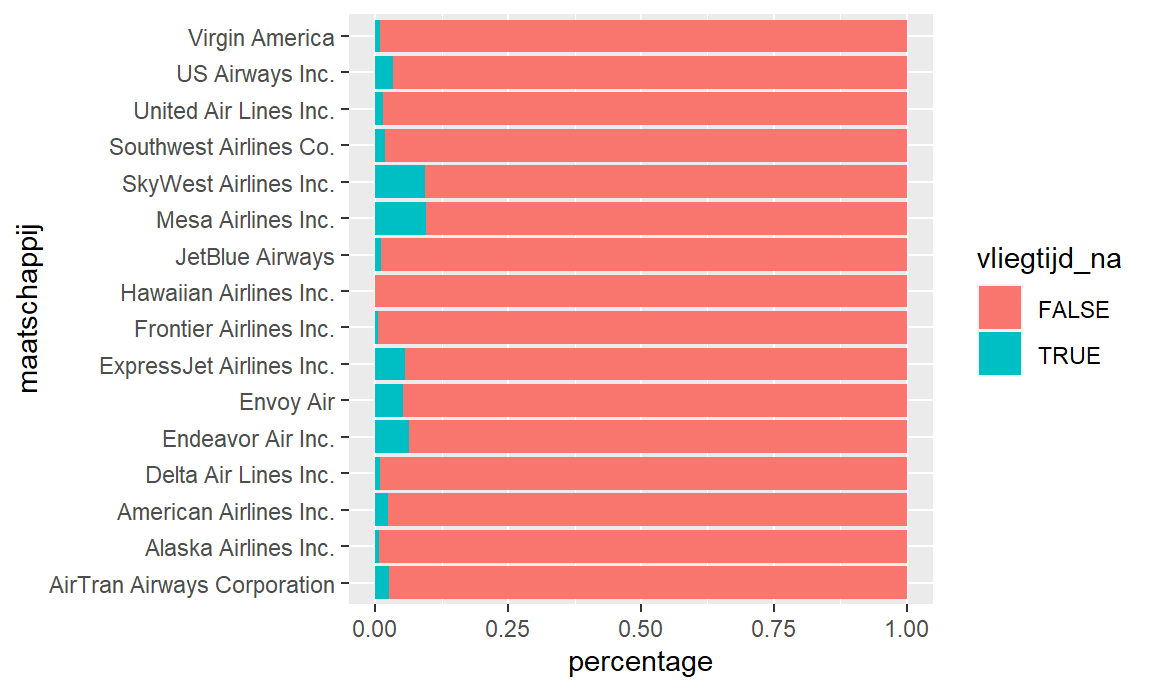
\includegraphics[width=0.49\linewidth]{lecture_notes_edda_files/figure-latex/5-19-1}

\begin{itemize}
\tightlist
\item
  Uit deze resultaten blijkt dat voor sommige maatschappijen een aanzienlijk hoger percentage ontbrekende waarden bij vliegtijd voorkomt (SkyWest, Mesa en ook ExpressJet, Envoy en Endeavor).
\item
  We kunnen een soortgelijke analyse ook uitvoeren voor de variabele \emph{afstand}. Hiervoor zullen we eerst de variabele \emph{afstand} omvormen tot een categorische variabele. We doen dit door de gehele deling uit te voeren (hiervoor gebruik je de \%/\% operator).
\end{itemize}

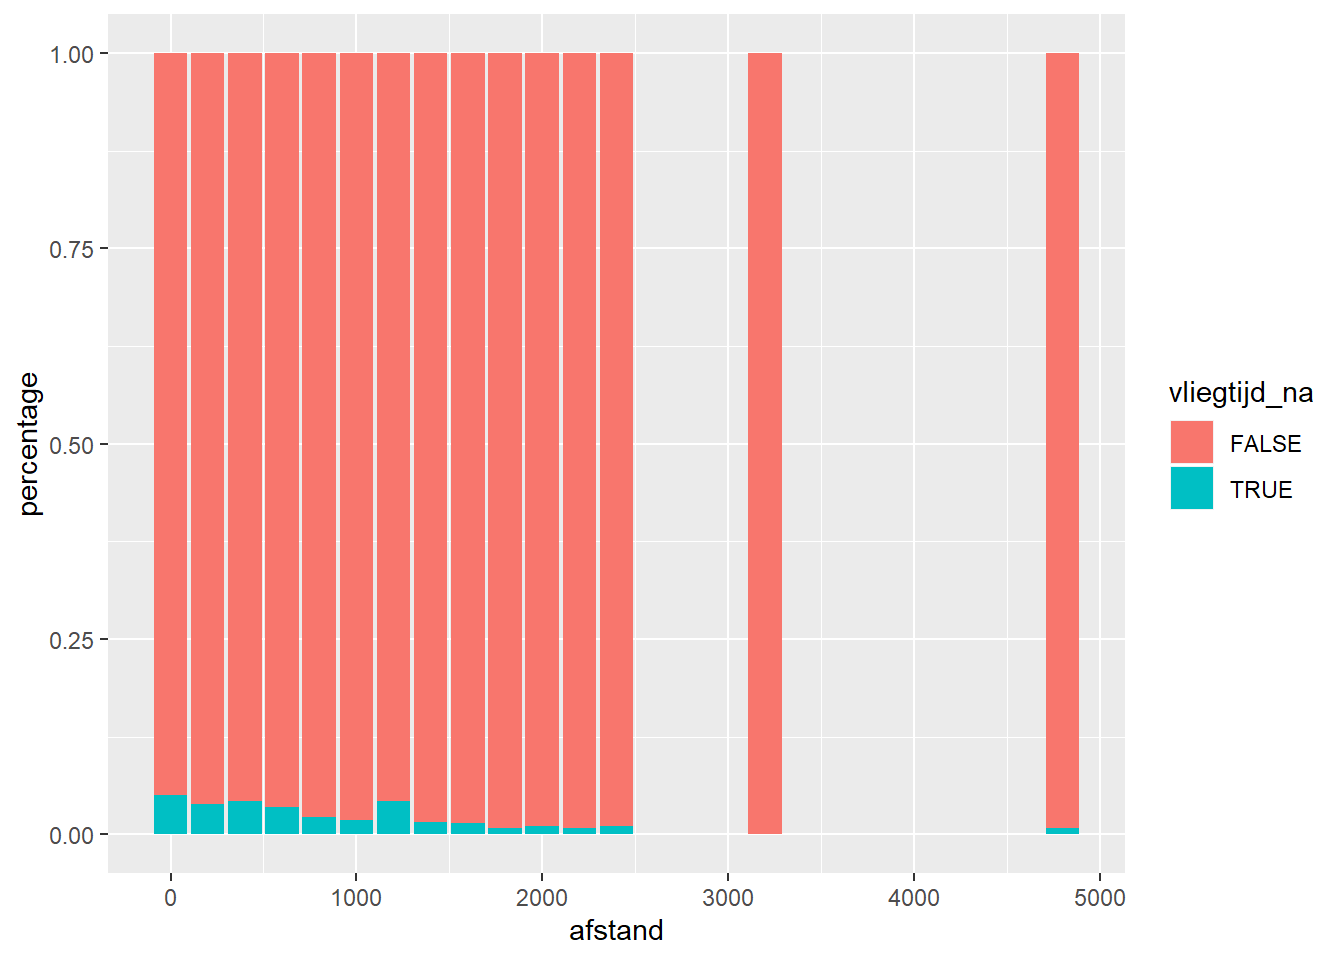
\includegraphics[width=0.49\linewidth]{lecture_notes_edda_files/figure-latex/5-20-1}

\begin{itemize}
\tightlist
\item
  Deze resultaten lijken te suggereren dat naarmate de vlucht langer wordt, het percentage ontbrekende waarden bij \emph{vliegtijd} afneemt (met een uitzonderlijke piek bij vluchten rond 1200 mijl).
\item
  Omdat het percentage ontbrekende waarden eerder klein is, is het moeilijk om het patroon duidelijk te zien. We kunnen ook dezelfde plot maken, maar de y-as laten stoppen bij een waarde van 0.25. Op deze manier wordt het patroon duidelijker.
\end{itemize}

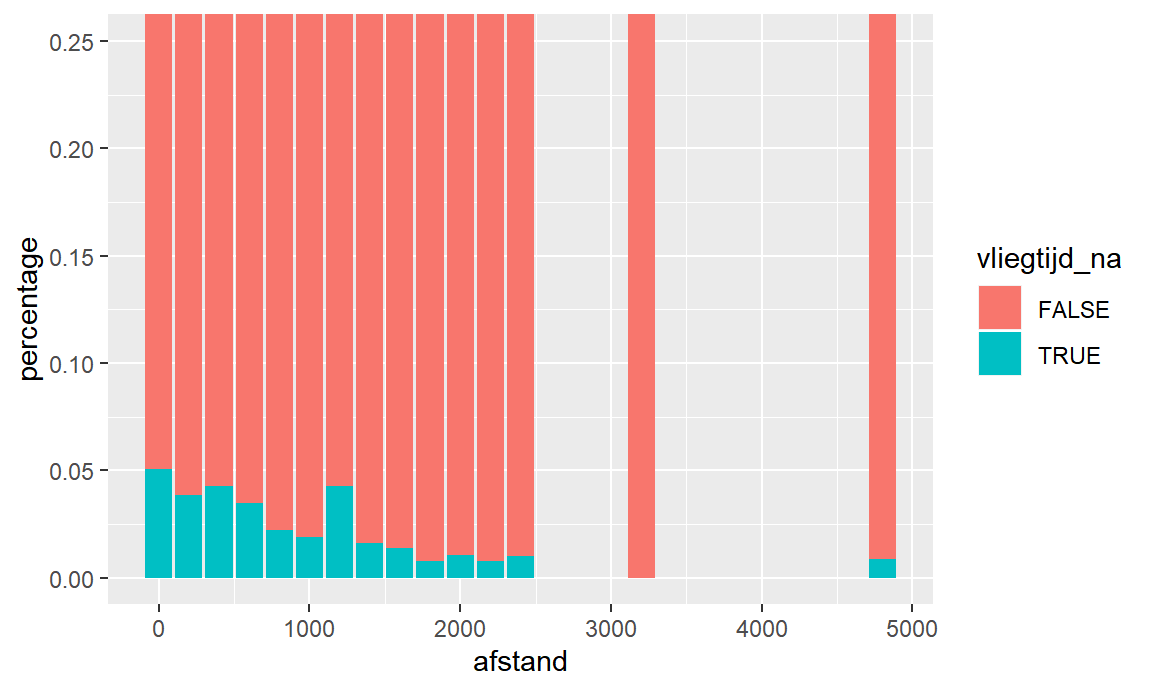
\includegraphics[width=0.49\linewidth]{lecture_notes_edda_files/figure-latex/5-21-1}

\begin{itemize}
\tightlist
\item
  Tenslotte kunnen we ook nog op een andere manier het verband tussen de \emph{afstand} en het voorkomen van ontbrekende waarden bij \emph{vliegtijd} bestuderen, nl. via 2 boxplots.
\end{itemize}

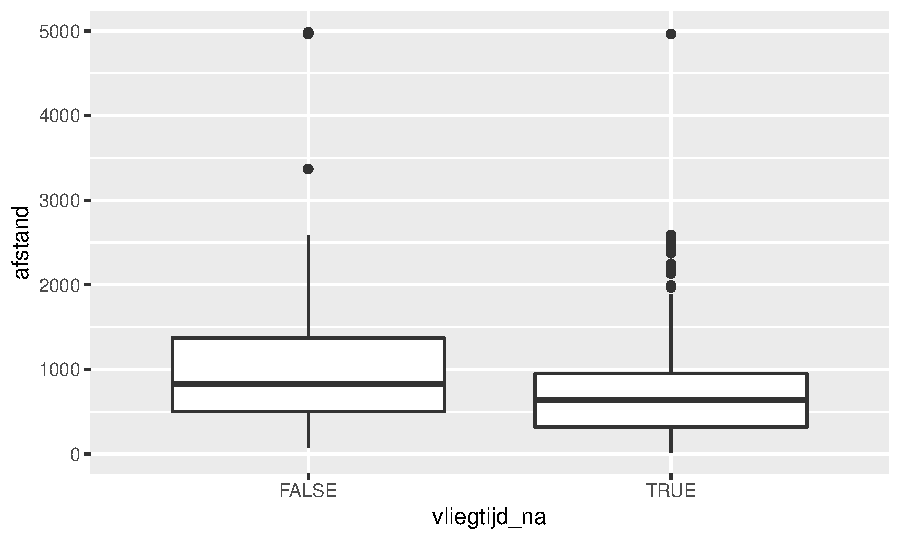
\includegraphics[width=0.49\linewidth]{lecture_notes_edda_files/figure-latex/5-22-1}

\begin{itemize}
\tightlist
\item
  Hier zien we dat vluchten waarvoor de vliegtijd ontbreekt vaak kortere vluchten zijn dan waarvoor we de vliegtijd wel hebben. Dit komt overeen met de vorige bevinding.
\item
  Op basis van deze resultaten kunnen we dus stellen dat het ontbreken van de vliegtijd niet willekeurig is, maar vaker voorkomt bij bepaalde maatschappijen en eerder bij kortere dan bij langere vluchten.
\item
  We zouden nog verder kunnen onderzoeken of deze maatschappijen eerder langere of kortere vluchten organiseren.
\item
  Soortgelijke analyses kunnen we ook uitvoeren voor de variabelen \emph{vertrek\_vertraging} en \emph{aankomst\_vertraging}.
\end{itemize}

\hypertarget{inconsistente-waarden}{%
\subsection{Inconsistente waarden}\label{inconsistente-waarden}}

\begin{itemize}
\tightlist
\item
  Data is inconsistent als het niet voldoet aan een aantal regels/beperkingen die horen te gelden op basis van domeinkennis.
\item
  De vorm van inconsistenties waar we ons op focussen, betreft in-record inconsistenties. Dit zijn tegenstrijdigheden die aanwezig zijn binnen één enkele observatie. Enkele voorbeelden zijn:

  \begin{itemize}
  \tightlist
  \item
    De gemiddelde snelheid van een vlucht ligt hoger dan de maximale theoretische snelheid van het vliegtuig.
  \item
    Het aankomsttijdstip van een vlucht vindt plaats voor het vertrektijdstip.
  \item
    De aankomsttijdstip komt niet overeen met het vertrektijdstip + vertrekvertraging + vluchtduur.
  \end{itemize}
\item
  Het identificeren van inconsistenties kan door middel van diverse dplyr-functies, waarbij je voor iedere observatie test of deze voldoen aan de opgelegde beperkingsregel.
\item
  Daarnaast is er ook het editrules package dat nuttige functies aanbiedt om op een gestructureerdere manier consistentie te evalueren.
\end{itemize}

\hypertarget{data-opwaarderen}{%
\section{Data opwaarderen}\label{data-opwaarderen}}

\begin{itemize}
\tightlist
\item
  Van zodra de data geen foutieve en/of ontbrekende waarde meer bevat, kunnen we een aantal technieken toepassen om de data bruikbaarder te maken voor exploratieve analyses. We onderscheiden hierbij 2 technieken:

  \begin{itemize}
  \tightlist
  \item
    Transformatie van bestaande variabelen.
  \item
    Selectie van observaties.
  \end{itemize}
\end{itemize}

\hypertarget{categorische-variabelen}{%
\subsubsection{Categorische variabelen}\label{categorische-variabelen}}

\begin{itemize}
\tightlist
\item
  Soms is het beter om de categorieën van een categorische variabelen te wijzigen door sommige categorieën samen te nemen. Er zijn verschillende situaties waarbij dit het overwegen waard is, zoals:

  \begin{itemize}
  \tightlist
  \item
    De labels van een categorische variabele is op een te gedetailleerd niveau gedefinieerd, met als gevolg dat de exploratieve analyse al snel complex wordt door de vele categorieën. In zulke gevallen kan het zinvol zijn om het aantal categorieën te verminderen door categorieën die inhoudelijk bij elkaar horen samen te nemen.
  \item
    Een categorische variabele bestaat uit een beperkt aantal categorieën met veel observaties en een groot aantal categorieën met zeer weinig observaties. In zulke gevallen kan het zinvol zijn om de categorieën met weinig observaties samen te nemen in 1 categorie ``Overige''.
  \end{itemize}
\item
  Om te bepalen welke categorieën men kan samenvoegen, kan een frequentietabel of barplot gemaakt worden.
\item
  Het herdefiniëren van de labels gebeurt vervolgens met de functie \emph{fct\_recode} (forcats). Hierbij heeft men steeds de keuze om de oorspronkelijke variabele te vervangen of een nieuwe variabele aan te maken.
\item
  Laten we eens aan de hand van een barplot naar de variabele `luchtvaartmaatschappij' kijken. We zien hierbij dat er relatief veel luchtvaartmaatschappijen (categorieën) in onze data zijn en dat er een aantal verwaarloosbaar weinig vluchten bevatten.
\end{itemize}

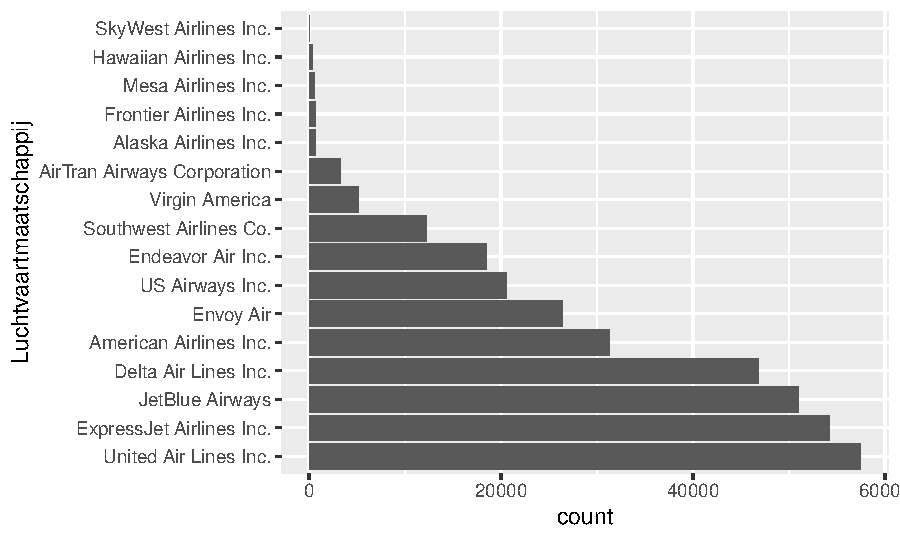
\includegraphics[width=0.49\linewidth]{lecture_notes_edda_files/figure-latex/5-21b-1}

\begin{itemize}
\tightlist
\item
  We kunnen de exacte aantallen achterhalen met behulp van een frequentietabel.
\end{itemize}

\begin{table}[t]

\caption{\label{tab:5-22b}Luchtvaartmaatschappijen geordend volgens stijgend aantal vluchten.}
\centering
\fontsize{10}{12}\selectfont
\begin{tabular}{lr}
\toprule
maatschappij & n\\
\midrule
SkyWest Airlines Inc. & 32\\
Hawaiian Airlines Inc. & 342\\
Mesa Airlines Inc. & 601\\
Frontier Airlines Inc. & 685\\
Alaska Airlines Inc. & 714\\
\addlinespace
AirTran Airways Corporation & 3260\\
Virgin America & 5162\\
Southwest Airlines Co. & 12275\\
Endeavor Air Inc. & 18460\\
US Airways Inc. & 20536\\
\addlinespace
Envoy Air & 26397\\
American Airlines Inc. & 31327\\
Delta Air Lines Inc. & 46779\\
JetBlue Airways & 50940\\
ExpressJet Airlines Inc. & 54173\\
\addlinespace
United Air Lines Inc. & 57491\\
\bottomrule
\end{tabular}
\end{table}

\begin{itemize}
\item
  Op basis van deze analyse beslissen we om de luchtvaartmaatschappijen met minder dan 10000 vluchten samen te voegen in een nieuwe categorie met het label ``Overige''. We opteren ervoor de oorspronkelijke variabelen te vervangen.
\item
  De nieuwe frequentietabel toont het resultaat.
\end{itemize}

\begin{table}[t]

\caption{\label{tab:5-24b}Luchtvaartmaatschappijen geordend volgens stijgend aantal vluchten.}
\centering
\fontsize{10}{12}\selectfont
\begin{tabular}{lr}
\toprule
maatschappij & n\\
\midrule
Overige & 10796\\
Southwest Airlines Co. & 12275\\
Endeavor Air Inc. & 18460\\
US Airways Inc. & 20536\\
Envoy Air & 26397\\
\addlinespace
American Airlines Inc. & 31327\\
Delta Air Lines Inc. & 46779\\
JetBlue Airways & 50940\\
ExpressJet Airlines Inc. & 54173\\
United Air Lines Inc. & 57491\\
\bottomrule
\end{tabular}
\end{table}

\hypertarget{continue-variabelen-1}{%
\subsubsection{Continue variabelen}\label{continue-variabelen-1}}

\begin{itemize}
\tightlist
\item
  Bij continue variabelen zijn er verschillende transformaties die regelmatig uitgevoerd worden:

  \begin{itemize}
  \tightlist
  \item
    De transformatie van een continue variabele naar een categorische variabele.
  \item
    Het herschalen van de continue variabele.
  \item
    De creatie van een nieuwe variabele op basis van bestaande continue variabelen.
  \end{itemize}
\item
  Ook hier hebben we weer steeds de mogelijkheid om de bestaande variabele te vervangen of een nieuwe variabele aan te maken.
\item
  Laten we de variabele vliegtijd eens onder de loep nemen. We beginnen met een visuele analyse aan de hand van een violinplot.
\end{itemize}

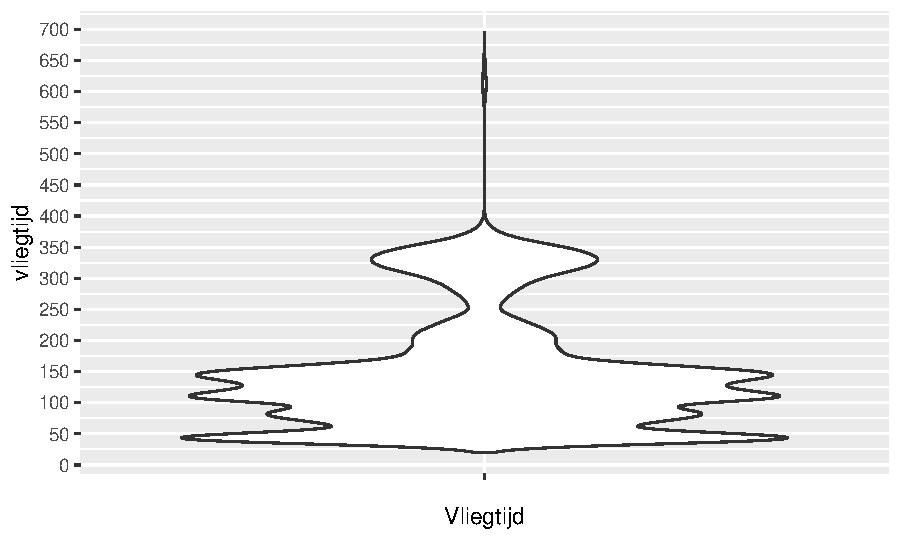
\includegraphics[width=0.49\linewidth]{lecture_notes_edda_files/figure-latex/5-25-1}

\begin{itemize}
\item
  Op basis van deze plot beslissen we een nieuwe categorische variabele ``vliegtijd\_fct'' aan te maken, waarbij `kort' overeenkomt met een vlucht die minder dan een uur duurt, `normaal' overeenkomt met een vlucht tussen 1 en 4 uur (60-240) en `lang' overeenkomt met een vlucht van meer dan 4 uur. Hiervoor maken we gebruik van de functie \emph{cut}.
\item
  Aan de hand van een frequentietabel kunnen we nu het resultaat bekijken.
\end{itemize}

\begin{table}[t]

\caption{\label{tab:5-27b}Frequentietabel vliegtijd (factor)}
\centering
\fontsize{10}{12}\selectfont
\begin{tabular}{lr}
\toprule
vliegtijd\_fct & n\\
\midrule
kort & 53220\\
normaal & 210758\\
lang & 55828\\
NA & 9368\\
\bottomrule
\end{tabular}
\end{table}

\begin{itemize}
\tightlist
\item
  Vervolgens beslissen we een nieuwe variabele te maken die de vliegtijd uitdrukt in uren in plaats van minuten.
\end{itemize}

\begin{Shaded}
\begin{Highlighting}[]
\NormalTok{df }\OperatorTok
\StringTok{  }\KeywordTok{mutate}\NormalTok{(}\DataTypeTok{vliegtijd_uren =}\NormalTok{ vliegtijd}\OperatorTok{/}\DecValTok{60}\NormalTok{) ->}\StringTok{ }\NormalTok{df}
\end{Highlighting}
\end{Shaded}

\begin{itemize}
\tightlist
\item
  We kunnen het resultaat bekijken met een violinplot.
\end{itemize}

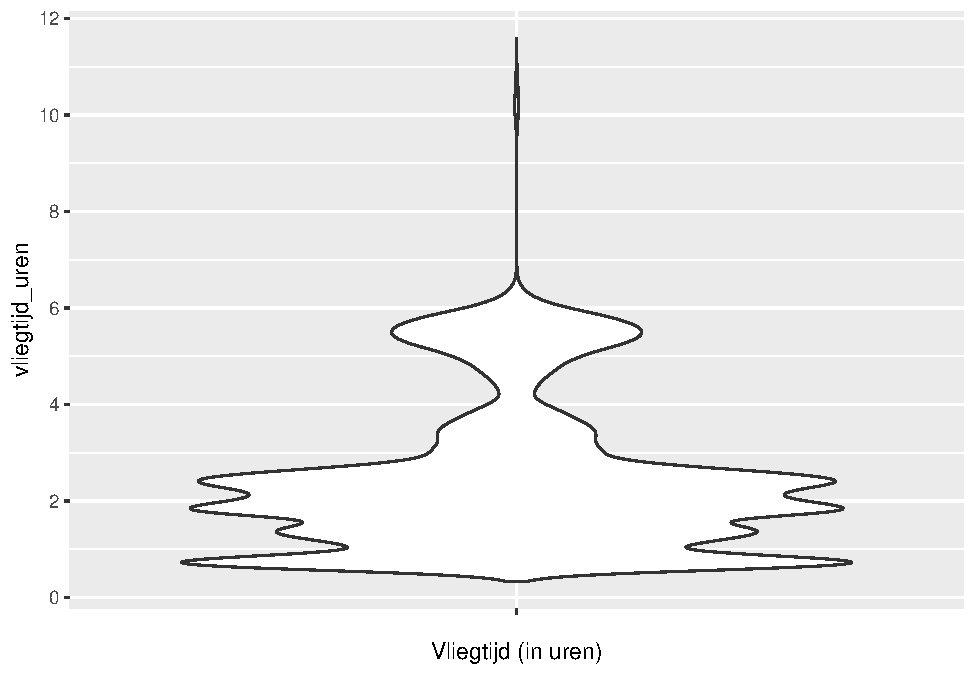
\includegraphics[width=0.49\linewidth]{lecture_notes_edda_files/figure-latex/5-29-1}

\begin{itemize}
\tightlist
\item
  Tenslotte maken we een nieuwe variabele die de gemiddelde snelheid van het vliegtuig uitdrukt door de afstand te delen door de vliegtijd.
\end{itemize}

\begin{Shaded}
\begin{Highlighting}[]
\NormalTok{df }\OperatorTok
\StringTok{  }\KeywordTok{mutate}\NormalTok{(}\DataTypeTok{snelheid =}\NormalTok{ afstand }\OperatorTok{/}\StringTok{ }\NormalTok{vliegtijd_uren) ->}\StringTok{ }\NormalTok{df}
\end{Highlighting}
\end{Shaded}

\begin{itemize}
\tightlist
\item
  Laten we het resultaat aan de hand van een histogram bekijken.
\end{itemize}

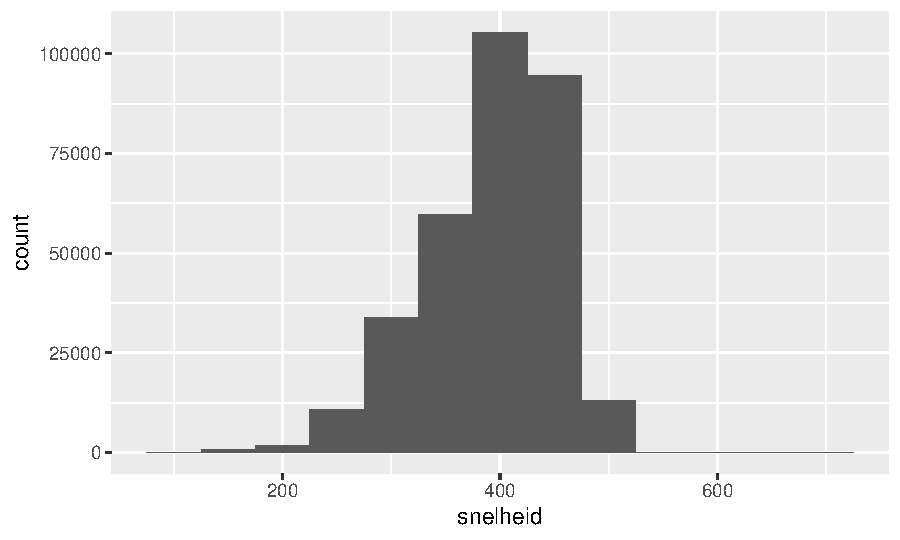
\includegraphics[width=0.49\linewidth]{lecture_notes_edda_files/figure-latex/5-31-1}

\hypertarget{sampling}{%
\subsection{Sampling}\label{sampling}}

\begin{itemize}
\tightlist
\item
  Soms is een dataset zo groot, dat analyses veel tijd in beslag nemen. In zulke gevallen kan het nuttig zijn om een random sample te nemen van de oorspronkelijke data om een eerste exploratieve analyse op uit te voeren.
\item
  Zolang de sample willekeurig getrokken wordt en de nieuwe dataset niet te klein wordt, is de kans dat je patronen ontdekt in de sample die niet voorkomen in de volledige dataset eerder klein.
\item
  Na een eerste exploratieve data analyse op de beperkte sample, kan men vervolgens gerichter de volledige dataset analyseren.
\item
  Laten we een sample van 10000 vluchten nemen uit de oorspronkelijke dataset.
\end{itemize}

\begin{Shaded}
\begin{Highlighting}[]
\NormalTok{df}\FloatTok{.10000}\NormalTok{ <-}\StringTok{ }\NormalTok{df }\OperatorTok\StringTok{ }\KeywordTok{sample_n}\NormalTok{(}\DecValTok{10000}\NormalTok{)}
\end{Highlighting}
\end{Shaded}

\begin{itemize}
\tightlist
\item
  We kunnen nu een eerste blik op deze sample werpen met behulp van de \emph{summary} functie.
\end{itemize}

\begin{verbatim}
##  luchthaven                   maatschappij  vertrek_vertraging
##  EWR:3728   ExpressJet Airlines Inc.:1723   Min.   :-25.00    
##  JFK:3107   United Air Lines Inc.   :1718   1st Qu.: -5.00    
##  LGA:3165   JetBlue Airways         :1528   Median : -2.00    
##             Delta Air Lines Inc.    :1479   Mean   : 13.07    
##             American Airlines Inc.  : 923   3rd Qu.: 10.00    
##             Envoy Air               : 798   Max.   :504.00    
##             (Other)                 :1831   NA's   :256       
##  aankomst_vertraging    afstand       vliegtijd    
##  Min.   :-67.00      Min.   :  80   Min.   : 23.0  
##  1st Qu.:-17.00      1st Qu.: 502   1st Qu.: 81.0  
##  Median : -5.00      Median : 820   Median :127.0  
##  Mean   :  7.42      Mean   :1020   Mean   :148.5  
##  3rd Qu.: 14.00      3rd Qu.:1215   3rd Qu.:181.0  
##  Max.   :448.00      Max.   :4983   Max.   :686.0  
##  NA's   :294                        NA's   :294    
##              vluchttype   vertrek_vertraging_na aankomst_vertraging_na
##  kort             :7504   Mode :logical         Mode :logical         
##  normaal          : 986   FALSE:9744            FALSE:9706            
##  lang             :1492   TRUE :256             TRUE :294             
##  intercontinentaal:  18                                               
##                                                                       
##                                                                       
##                                                                       
##  vliegtijd_na    vliegtijd_fct  vliegtijd_uren       snelheid    
##  Mode :logical   kort   :1586   Min.   : 0.3833   Min.   :120.0  
##  FALSE:9706      normaal:6467   1st Qu.: 1.3500   1st Qu.:356.6  
##  TRUE :294       lang   :1653   Median : 2.1167   Median :402.6  
##                  NA's   : 294   Mean   : 2.4746   Mean   :392.3  
##                                 3rd Qu.: 3.0167   3rd Qu.:435.9  
##                                 Max.   :11.4333   Max.   :550.6  
##                                 NA's   :294       NA's   :294
\end{verbatim}

\begin{itemize}
\tightlist
\item
  Als we dit vergelijken met de volledige dataset, dan zien we relatief weinig verschillen wat betreft de centrummaten en de robuste spreidingsmaten.
\item
  Merk op dat minima's en maxima's wel sterk kunnen verschillen. Dit is omdat dit geen robuste maatstaven zijn.
\end{itemize}

\begin{verbatim}
##  luchthaven                     maatschappij   vertrek_vertraging
##  EWR:119282   United Air Lines Inc.   :57491   Min.   : -43.00   
##  JFK:105230   ExpressJet Airlines Inc.:54173   1st Qu.:  -5.00   
##  LGA:104662   JetBlue Airways         :50940   Median :  -2.00   
##               Delta Air Lines Inc.    :46779   Mean   :  12.71   
##               American Airlines Inc.  :31327   3rd Qu.:  11.00   
##               Envoy Air               :26397   Max.   :1301.00   
##               (Other)                 :62067   NA's   :8214      
##  aankomst_vertraging    afstand       vliegtijd    
##  Min.   : -86.000    Min.   :  17   Min.   : 20.0  
##  1st Qu.: -17.000    1st Qu.: 502   1st Qu.: 81.0  
##  Median :  -5.000    Median : 820   Median :127.0  
##  Mean   :   6.987    Mean   :1027   Mean   :149.6  
##  3rd Qu.:  14.000    3rd Qu.:1372   3rd Qu.:184.0  
##  Max.   :1272.000    Max.   :4983   Max.   :695.0  
##  NA's   :9365                       NA's   :9368   
##              vluchttype     vertrek_vertraging_na aankomst_vertraging_na
##  kort             :245666   Mode :logical         Mode :logical         
##  normaal          : 31813   FALSE:320960          FALSE:319809          
##  lang             : 50980   TRUE :8214            TRUE :9365            
##  intercontinentaal:   715                                               
##                                                                         
##                                                                         
##                                                                         
##  vliegtijd_na    vliegtijd_fct    vliegtijd_uren      snelheid    
##  Mode :logical   kort   : 53220   Min.   : 0.333   Min.   : 76.8  
##  FALSE:319806    normaal:210758   1st Qu.: 1.350   1st Qu.:356.3  
##  TRUE :9368      lang   : 55828   Median : 2.117   Median :402.6  
##                  NA's   :  9368   Mean   : 2.493   Mean   :392.1  
##                                   3rd Qu.: 3.067   3rd Qu.:436.2  
##                                   Max.   :11.583   Max.   :703.4  
##                                   NA's   :9368     NA's   :9368
\end{verbatim}

\hypertarget{referenties-3}{%
\section*{Referenties}\label{referenties-3}}
\addcontentsline{toc}{section}{Referenties}

\begin{enumerate}
\def\labelenumi{\arabic{enumi}.}
\tightlist
\item
  \href{http://kunststube.net/encoding/}{Encoding}
\item
  \href{https://www.joelonsoftware.com/2003/10/08/the-absolute-minimum-every-software-developer-absolutely-positively-must-know-about-unicode-and-character-sets-no-excuses/}{De geschiedenis van ASCII}
\item
  \href{https://en.wikipedia.org/wiki/Windows_code_page}{Windows code pages}
\item
  \href{http://r4ds.had.co.nz/data-import.html}{Data importeren in R}
\item
  \href{https://www.techwalla.com/articles/what-is-a-delimited-a-fixed-width-file}{Delimited en fixed-width bestanden}
\item
  \href{https://www.w3schools.com/xml/default.asp}{XML}
\item
  \href{http://beginnersbook.com/2015/04/json-tutorial/}{JSON Tutorial}
\item
  \href{https://chemicalstatistician.wordpress.com/2018/03/10/use-unique-instead-of-levels-to-find-the-possible-values-of-a-character-variable-in-r/}{Unique-functie}
\item
  \href{http://r4ds.had.co.nz/factors.html}{Factors}
\item
  \href{http://forcats.tidyverse.org/reference/fct_relevel.html}{Fct\_relevel}
\item
  \href{http://rforpublichealth.blogspot.be/2012/09/from-continuous-to-categorical.html}{From continuous to categorical}
\end{enumerate}

\hypertarget{exploratieve-analyse-van-tijdgerelateerde-data}{%
\chapter{Exploratieve analyse van tijdgerelateerde data}\label{exploratieve-analyse-van-tijdgerelateerde-data}}

\hypertarget{inleiding}{%
\section{Inleiding}\label{inleiding}}

\hypertarget{tijdstippen-versus-periodes}{%
\subsection{Tijdstippen versus periodes}\label{tijdstippen-versus-periodes}}

\begin{itemize}
\tightlist
\item
  We kunnen tijdgerelateerde data in twee categorieën onderverdelen: tijdstippen en periodes.
\item
  Tijdstip.

  \begin{itemize}
  \tightlist
  \item
    Verwijst naar een specifiek moment in de tijd.
  \item
    3 varianten:

    \begin{itemize}
    \tightlist
    \item
      datum (``01-01-2017'') verwijst naar een specifieke dag.
    \item
      datum-tijdstip (``01-01-2017 13:54'') verwijst naar een specifiek moment op een specifieke dag.
    \item
      tijdstip (``13:54'') verwijst naar een specifiek moment op een ongedefinieerde dag.
    \end{itemize}
  \end{itemize}
\item
  Periode.

  \begin{itemize}
  \tightlist
  \item
    Verwijst naar een periode en wordt typisch uitgedrukt aan de hand van de duur van de periode.

    \begin{itemize}
    \tightlist
    \item
      Bijvoorbeeld: Een periode van ``3605 seconden''" of een periode van ``2 maanden en 1 dag''.
    \end{itemize}
  \item
    Soms wordt een periode specifiek gedefinieerd aan de hand van twee specifieke tijdstippen die het begin en het einde van de periode aangeven.

    \begin{itemize}
    \tightlist
    \item
      Bijvoorbeeld: De periode van 01-01-2017 tot 03-01-2017.
    \end{itemize}
  \end{itemize}
\item
  \textbf{Bestudeer hoofdstuk 16 van het boek `R for Data Science' van Grolemund en Wickham !}
\end{itemize}

\hypertarget{tijdstippen}{%
\section{Tijdstippen}\label{tijdstippen}}

\hypertarget{creatie-van-tijdstippen}{%
\subsection{Creatie van tijdstippen}\label{creatie-van-tijdstippen}}

\begin{itemize}
\tightlist
\item
  Opdat R correct met tijdstippen omgaat, is het belangrijk dat tijdstip-variabelen ook correct als tijdstippen herkend worden.
\item
  Er zijn verschillende manieren om tijdstippen te creëren in R.

  \begin{itemize}
  \tightlist
  \item
    Op basis van het huidige tijdstip.

    \begin{itemize}
    \tightlist
    \item
      Dit is mogelijk met de functies \emph{today()} en \emph{now()} om respectievelijk een tijdstip van de huidige dag (datum) of het huidige tijdstip (datum\_tijd) aan te maken.
    \end{itemize}
  \item
    Op basis van karakterstring. Indien men reeds tijdstippen heeft in de dataset, maar deze zijn gecodeerd als karakterstrings, dan voorziet de \emph{lubridate} package een aantal handige functies hiervoor:

    \begin{itemize}
    \tightlist
    \item
      \emph{ymd()}, \emph{ydm()}, \emph{mdy()}, \emph{myd()}, \emph{dmy()}, \emph{dym()} voor datum-tijdstippen.
    \item
      \emph{ymd\_hms()}, \emph{ymd\_hm()}, \emph{ymd\_h()}, \emph{dmy\_hms()}, \emph{dmy\_hm()}, \emph{dmy\_h()}, \emph{mdy\_hms()}, \emph{mdy\_hm()}, \emph{mdy\_h()}, \emph{ydm\_hms()}, \emph{ydm\_hm()}, \emph{ydm\_hm()} voor datumtijd-tijdstippen.
    \item
      Al deze functies omschrijven de structuur van de karakterstring, waarbij \emph{y} voor jaar staat, de eerste \emph{m} voor maand, \emph{d} voor dag, \emph{h} voor uur, de tweede \emph{m} voor minuten en \emph{s} voor seconden.

      \begin{itemize}
      \tightlist
      \item
        Om de karakterstring ``2017-21-02 5:15'' correct om te zetten naar een tijdstip, moet je dus de functie \emph{ydm\_hm()} gebruiken.
      \end{itemize}
    \end{itemize}
  \item
    Op basis van verschillende variabelen die ieder een verschillende component (jaar, maand, dag, uur, minuten, seconden) bevatten.

    \begin{itemize}
    \tightlist
    \item
      Hiervoor kan je de functies `make\_date()' of `make\_datetime()' gebruiken, afhankelijk of je een datum- of een datumtijd-tijdstip wenst aan te maken.
    \end{itemize}
  \end{itemize}
\end{itemize}

\hypertarget{extractie-van-tijdstipinformatie}{%
\subsection{Extractie van tijdstipinformatie}\label{extractie-van-tijdstipinformatie}}

\begin{itemize}
\tightlist
\item
  Eénmaal variabelen in R als tijdstippen gecodeerd zijn, is het eenvoudig om de verschillende componenten hieruit te extraheren.
\item
  De componenten die je onmiddellijk op het oog kunt herkennen in de oorspronkelijke karakterstring zijn te extraheren met de volgende functies:

  \begin{itemize}
  \tightlist
  \item
    \emph{year()}.
  \item
    \emph{month()}.
  \item
    \emph{mday()}.
  \item
    \emph{hour()}.
  \item
    \emph{minute()}.
  \item
    \emph{second()}.
  \end{itemize}
\item
  Daarnaast zijn er ook andere componenten die je uit een tijdstip kunt extraheren, dewelke niet rechtstreeks af te lezen zijn uit de oorspronkelijke karakterstring.

  \begin{itemize}
  \tightlist
  \item
    \emph{week()}: De week van het jaar. ``5 feb 2017'' is bijvoorbeeld de 6de week van het jaar.
  \item
    \emph{yday()}: De dag in het jaar. ``5 feb 2017'' is bijvoorbeeld de 36ste dag van het jaar.
  \item
    \emph{wday()}: De dag van de week. ``5 feb 2017'' is bijvoorbeeld de eerste dag van de week. Let wel op dat we hierbij de conventie hanteren dat een week op zondag start.
  \item
    \emph{wday(\ldots{}, label=TRUE)}: De naam van de dag van de week. ``5 feb 2017'' is bijvoorbeeld zondag.
  \end{itemize}
\end{itemize}

\hypertarget{afronden-van-tijdstippen}{%
\subsection{Afronden van tijdstippen}\label{afronden-van-tijdstippen}}

\begin{itemize}
\tightlist
\item
  Ieder tijdstip heeft een zekere nauwkeurigheid. Sommige tijdstippen zijn tot op de seconde gedefinieerd terwijl andere slechts een nauwkeurigheid hebben van weken of maanden.
\item
  Soms kan het voor visualisaties of analyses zinvol zijn om tijdstippen minder nauwkeurig te maken en deze af te ronden. Hiervoor zijn er drie mogelijke functies, afhankelijk van het soort afronding dat men wenst.

  \begin{itemize}
  \tightlist
  \item
    floor\_date(): afronden naar onder toe.
  \item
    round\_date(): normale afrondingsregels.
  \item
    ceiling\_date(): afronden naar boven toe.
  \end{itemize}
\item
  Deze drie functies hebben 1 belangrijke parameter (unit) waarmee je het afrondingsniveau kunt bepalen.
\end{itemize}

\hypertarget{case-nyc-vluchten-2013}{%
\subsection{Case: NYC Vluchten 2013}\label{case-nyc-vluchten-2013}}

\begin{itemize}
\tightlist
\item
  We zullen de concepten omtrent tijdgerelateerde data illustreren aan de hand van een dataset over de vluchten vanuit NYC in 2013.
\item
  Hieronder vind je een samenvatting van de verschillende variabelen die aanwezig zijn in de dataset.
\end{itemize}

\begin{verbatim}
## Observations: 319,809
## Variables: 12
## $ vertrekluchthaven   <chr> "EWR", "LGA", "JFK", "LGA", "EWR", "EWR", ...
## $ aankomstluchthaven  <chr> "George Bush Intercontinental", "George Bu...
## $ maatschappij        <chr> "United Air Lines Inc.", "United Air Lines...
## $ jaar_vertrek        <int> 2013, 2013, 2013, 2013, 2013, 2013, 2013, ...
## $ maand_vertrek       <int> 1, 1, 1, 1, 1, 1, 1, 1, 1, 1, 1, 1, 1, 1, ...
## $ dag_vertrek         <int> 1, 1, 1, 1, 1, 1, 1, 1, 1, 1, 1, 1, 1, 1, ...
## $ uur_vertrek         <dbl> 5, 5, 5, 5, 5, 5, 5, 5, 5, 5, 5, 5, 5, 5, ...
## $ minuut_vertrek      <dbl> 17, 33, 42, 54, 54, 55, 57, 57, 58, 58, 58...
## $ tijdstip_aankomst   <chr> "2013-01-01 08:30:00", "2013-01-01 08:50:0...
## $ vertrek_vertraging  <dbl> 2, 4, 2, -6, -4, -5, -3, -3, -2, -2, -2, -...
## $ aankomst_vertraging <dbl> 11, 20, 33, -25, 12, 19, -14, -8, 8, -2, -...
## $ afstand             <dbl> 1400, 1416, 1089, 762, 719, 1065, 229, 944...
\end{verbatim}

\begin{itemize}
\tightlist
\item
  Allereerst willen we de variabele \emph{tijdstip\_aankomst} omzetten van een karakterstring naar een datumtijd tijdstip.
\end{itemize}

\begin{Shaded}
\begin{Highlighting}[]
\NormalTok{df }\OperatorTok\StringTok{ }
\StringTok{  }\KeywordTok{mutate}\NormalTok{(}\DataTypeTok{tijdstip_aankomst =} \KeywordTok{ymd_hms}\NormalTok{(tijdstip_aankomst)) ->}\StringTok{ }\NormalTok{df}
\KeywordTok{glimpse}\NormalTok{(df)}
\end{Highlighting}
\end{Shaded}

\begin{verbatim}
## Observations: 319,809
## Variables: 12
## $ vertrekluchthaven   <chr> "EWR", "LGA", "JFK", "LGA", "EWR", "EWR", ...
## $ aankomstluchthaven  <chr> "George Bush Intercontinental", "George Bu...
## $ maatschappij        <chr> "United Air Lines Inc.", "United Air Lines...
## $ jaar_vertrek        <int> 2013, 2013, 2013, 2013, 2013, 2013, 2013, ...
## $ maand_vertrek       <int> 1, 1, 1, 1, 1, 1, 1, 1, 1, 1, 1, 1, 1, 1, ...
## $ dag_vertrek         <int> 1, 1, 1, 1, 1, 1, 1, 1, 1, 1, 1, 1, 1, 1, ...
## $ uur_vertrek         <dbl> 5, 5, 5, 5, 5, 5, 5, 5, 5, 5, 5, 5, 5, 5, ...
## $ minuut_vertrek      <dbl> 17, 33, 42, 54, 54, 55, 57, 57, 58, 58, 58...
## $ tijdstip_aankomst   <dttm> 2013-01-01 08:30:00, 2013-01-01 08:50:00,...
## $ vertrek_vertraging  <dbl> 2, 4, 2, -6, -4, -5, -3, -3, -2, -2, -2, -...
## $ aankomst_vertraging <dbl> 11, 20, 33, -25, 12, 19, -14, -8, 8, -2, -...
## $ afstand             <dbl> 1400, 1416, 1089, 762, 719, 1065, 229, 944...
\end{verbatim}

\begin{itemize}
\tightlist
\item
  Verder willen we ook een nieuwe variabele \emph{tijdstip\_vertrek} aanmaken op basis van de variabelen \emph{jaar\_vertrek}, \emph{maand\_vertrek}, \emph{dag\_vertrek}, \emph{uur\_vertrek} en \emph{minuut\_vertrek}.
\end{itemize}

\begin{Shaded}
\begin{Highlighting}[]
\NormalTok{df }\OperatorTok
\StringTok{  }\KeywordTok{mutate}\NormalTok{(}\DataTypeTok{tijdstip_vertrek =} \KeywordTok{make_datetime}\NormalTok{(jaar_vertrek, }
\NormalTok{                                          maand_vertrek, }
\NormalTok{                                          dag_vertrek, }
\NormalTok{                                          uur_vertrek, }
\NormalTok{                                          minuut_vertrek)) }\OperatorTok
\StringTok{  }\KeywordTok{select}\NormalTok{(}\OperatorTok{-}\StringTok{ }\NormalTok{jaar_vertrek, }
         \OperatorTok{-}\NormalTok{maand_vertrek, }
         \OperatorTok{-}\NormalTok{dag_vertrek, }
         \OperatorTok{-}\NormalTok{uur_vertrek, }
         \OperatorTok{-}\NormalTok{minuut_vertrek) ->}\StringTok{ }\NormalTok{df}
\KeywordTok{glimpse}\NormalTok{(df)}
\end{Highlighting}
\end{Shaded}

\begin{verbatim}
## Observations: 319,809
## Variables: 8
## $ vertrekluchthaven   <chr> "EWR", "LGA", "JFK", "LGA", "EWR", "EWR", ...
## $ aankomstluchthaven  <chr> "George Bush Intercontinental", "George Bu...
## $ maatschappij        <chr> "United Air Lines Inc.", "United Air Lines...
## $ tijdstip_aankomst   <dttm> 2013-01-01 08:30:00, 2013-01-01 08:50:00,...
## $ vertrek_vertraging  <dbl> 2, 4, 2, -6, -4, -5, -3, -3, -2, -2, -2, -...
## $ aankomst_vertraging <dbl> 11, 20, 33, -25, 12, 19, -14, -8, 8, -2, -...
## $ afstand             <dbl> 1400, 1416, 1089, 762, 719, 1065, 229, 944...
## $ tijdstip_vertrek    <dttm> 2013-01-01 05:17:00, 2013-01-01 05:33:00,...
\end{verbatim}

\begin{itemize}
\tightlist
\item
  Vervolgens willen we graag enkele nieuwe variabelen aanmaken die de volgende informatie bevatten: de weekdag van vertrek (maandag, dinsdag, \ldots{}), de week van vertrek, de maand van vertrek en de maanddag (1, 2, \ldots{}, 31) van vertrek.
\end{itemize}

\begin{Shaded}
\begin{Highlighting}[]
\NormalTok{df }\OperatorTok
\StringTok{  }\KeywordTok{mutate}\NormalTok{(}\DataTypeTok{weekdag_vertrek =} \KeywordTok{wday}\NormalTok{(tijdstip_vertrek, }\DataTypeTok{label =}\NormalTok{ T),}
         \DataTypeTok{week_vertrek =} \KeywordTok{week}\NormalTok{(tijdstip_vertrek),}
         \DataTypeTok{maand_vertrek =} \KeywordTok{month}\NormalTok{(tijdstip_vertrek),}
         \DataTypeTok{maanddag_vertrek =} \KeywordTok{mday}\NormalTok{(tijdstip_vertrek)) ->}\StringTok{ }\NormalTok{df}
\KeywordTok{glimpse}\NormalTok{(df)}
\end{Highlighting}
\end{Shaded}

\begin{verbatim}
## Observations: 319,809
## Variables: 12
## $ vertrekluchthaven   <chr> "EWR", "LGA", "JFK", "LGA", "EWR", "EWR", ...
## $ aankomstluchthaven  <chr> "George Bush Intercontinental", "George Bu...
## $ maatschappij        <chr> "United Air Lines Inc.", "United Air Lines...
## $ tijdstip_aankomst   <dttm> 2013-01-01 08:30:00, 2013-01-01 08:50:00,...
## $ vertrek_vertraging  <dbl> 2, 4, 2, -6, -4, -5, -3, -3, -2, -2, -2, -...
## $ aankomst_vertraging <dbl> 11, 20, 33, -25, 12, 19, -14, -8, 8, -2, -...
## $ afstand             <dbl> 1400, 1416, 1089, 762, 719, 1065, 229, 944...
## $ tijdstip_vertrek    <dttm> 2013-01-01 05:17:00, 2013-01-01 05:33:00,...
## $ weekdag_vertrek     <ord> Tue, Tue, Tue, Tue, Tue, Tue, Tue, Tue, Tu...
## $ week_vertrek        <dbl> 1, 1, 1, 1, 1, 1, 1, 1, 1, 1, 1, 1, 1, 1, ...
## $ maand_vertrek       <dbl> 1, 1, 1, 1, 1, 1, 1, 1, 1, 1, 1, 1, 1, 1, ...
## $ maanddag_vertrek    <int> 1, 1, 1, 1, 1, 1, 1, 1, 1, 1, 1, 1, 1, 1, ...
\end{verbatim}

\begin{itemize}
\tightlist
\item
  Tenslotte zullen we een nieuwe variabele maken dewelke het vertrekmoment afrondt tot op de dag nauwkeurig (dus zonder het specifieke uur).
\end{itemize}

\begin{Shaded}
\begin{Highlighting}[]
\NormalTok{df }\OperatorTok
\StringTok{  }\KeywordTok{mutate}\NormalTok{(}\DataTypeTok{dag_vertrek =} \KeywordTok{floor_date}\NormalTok{(tijdstip_vertrek, }\StringTok{"day"}\NormalTok{)) ->}\StringTok{ }\NormalTok{df}
\KeywordTok{glimpse}\NormalTok{(df)}
\end{Highlighting}
\end{Shaded}

\begin{verbatim}
## Observations: 319,809
## Variables: 13
## $ vertrekluchthaven   <chr> "EWR", "LGA", "JFK", "LGA", "EWR", "EWR", ...
## $ aankomstluchthaven  <chr> "George Bush Intercontinental", "George Bu...
## $ maatschappij        <chr> "United Air Lines Inc.", "United Air Lines...
## $ tijdstip_aankomst   <dttm> 2013-01-01 08:30:00, 2013-01-01 08:50:00,...
## $ vertrek_vertraging  <dbl> 2, 4, 2, -6, -4, -5, -3, -3, -2, -2, -2, -...
## $ aankomst_vertraging <dbl> 11, 20, 33, -25, 12, 19, -14, -8, 8, -2, -...
## $ afstand             <dbl> 1400, 1416, 1089, 762, 719, 1065, 229, 944...
## $ tijdstip_vertrek    <dttm> 2013-01-01 05:17:00, 2013-01-01 05:33:00,...
## $ weekdag_vertrek     <ord> Tue, Tue, Tue, Tue, Tue, Tue, Tue, Tue, Tu...
## $ week_vertrek        <dbl> 1, 1, 1, 1, 1, 1, 1, 1, 1, 1, 1, 1, 1, 1, ...
## $ maand_vertrek       <dbl> 1, 1, 1, 1, 1, 1, 1, 1, 1, 1, 1, 1, 1, 1, ...
## $ maanddag_vertrek    <int> 1, 1, 1, 1, 1, 1, 1, 1, 1, 1, 1, 1, 1, 1, ...
## $ dag_vertrek         <dttm> 2013-01-01, 2013-01-01, 2013-01-01, 2013-...
\end{verbatim}

\hypertarget{periode-data}{%
\section{Periode-data}\label{periode-data}}

\begin{itemize}
\tightlist
\item
  We kunnen 3 soorten van periodes onderscheiden, waarbij het eerste type (interval) naar een specifieke periode tussen 2 tijdstippen verwijst en de 2 andere types (\emph{duration} en \emph{period}) naar een periode van een specifieke duur verwijzen maar telkens onafhankelijk van het specifieke tijdstip.
\item
  Om de verschillen duidelijk te illustreren werken we met twee specifieke tijdstippen ``1 jan 2016'' en ``1 jan 2017''.
\end{itemize}

\begin{Shaded}
\begin{Highlighting}[]
\NormalTok{t1 <-}\StringTok{ }\KeywordTok{ymd}\NormalTok{(}\DecValTok{160101}\NormalTok{)}
\NormalTok{t1}
\end{Highlighting}
\end{Shaded}

\begin{verbatim}
## [1] "2016-01-01"
\end{verbatim}

\begin{Shaded}
\begin{Highlighting}[]
\NormalTok{t2 <-}\StringTok{ }\KeywordTok{ymd}\NormalTok{(}\DecValTok{170101}\NormalTok{)}
\NormalTok{t2}
\end{Highlighting}
\end{Shaded}

\begin{verbatim}
## [1] "2017-01-01"
\end{verbatim}

\hypertarget{interval-1}{%
\subsection{Interval}\label{interval-1}}

\begin{itemize}
\tightlist
\item
  Een interval is een periode die bepaald wordt door twee specifieke tijdstippen.
\item
  Een interval creëer je met behulp van de speciale operator \texttt{\%-\/-\%}.
\item
  Intervals worden weinig gebruikt om rechtstreeks te analyseren, maar kunnen als tussenstap gebruikt worden om de duurtijd van specifieke periodes te bepalen.
\end{itemize}

\begin{Shaded}
\begin{Highlighting}[]
\NormalTok{interval_t2t1 <-}\StringTok{ }\NormalTok{t1 }\OperatorTok\StringTok{ }\NormalTok{t2}
\NormalTok{interval_t2t1}
\end{Highlighting}
\end{Shaded}

\begin{verbatim}
## [1] 2016-01-01 UTC--2017-01-01 UTC
\end{verbatim}

\hypertarget{duration}{%
\subsection{Duration}\label{duration}}

\begin{itemize}
\tightlist
\item
  Duration is de duur van een periode uitgedrukt als het exact aantal seconden die feitelijk verstreken zijn tussen twee tijdstippen.
\item
  Tussen `26 maart 2017 02:00:00' en `26 maart 2017 03:00:01' is slechts 1 seconde feitelijk verstreken omdat we van 2u naar 3u zijn overgeschakeld op het zomeruur.
\item
  Durations gebruik je voornamelijk als je de werkelijke tijd tussen twee tijdstippen wenst te berekenen of wanneer je een aantal seconden wenst toe te voegen bij of af te trekken van een specifiek tijdstip.
\item
  Om een duration van een specifieke duur te creëren gebruik je volgende functies:

  \begin{itemize}
  \tightlist
  \item
    \emph{dseconds()}.
  \item
    \emph{dminutes()}.
  \item
    \emph{dhours()}.
  \item
    \emph{ddays()}.
  \item
    \emph{dweeks()}.
  \item
    \emph{dyears()}.
  \end{itemize}
\item
  Om de duration van een interval te bepalen, gebruik je de functie:

  \begin{itemize}
  \tightlist
  \item
    \emph{as.duration()}.
  \end{itemize}
\end{itemize}

\begin{Shaded}
\begin{Highlighting}[]
\NormalTok{t1 }\OperatorTok{+}\StringTok{ }\KeywordTok{dyears}\NormalTok{(}\DecValTok{1}\NormalTok{)}
\end{Highlighting}
\end{Shaded}

\begin{verbatim}
## [1] "2016-12-31"
\end{verbatim}

\begin{Shaded}
\begin{Highlighting}[]
\NormalTok{interval_t2t1 }\OperatorTok{/}\StringTok{ }\KeywordTok{dyears}\NormalTok{(}\DecValTok{1}\NormalTok{)}
\end{Highlighting}
\end{Shaded}

\begin{verbatim}
## [1] 1.00274
\end{verbatim}

\begin{Shaded}
\begin{Highlighting}[]
\KeywordTok{as.duration}\NormalTok{(interval_t2t1)}
\end{Highlighting}
\end{Shaded}

\begin{verbatim}
## [1] "31622400s (~1 years)"
\end{verbatim}

\hypertarget{period}{%
\subsection{Period}\label{period}}

\begin{itemize}
\tightlist
\item
  De tijd die verstreken `lijkt' te zijn (op een klok) tussen twee tijdstippen.
\item
  Dus tussen `26 maart 2017 02:00:00' en `26 maart 2017 03:00:01' zit een period van 1 uur en 1 seconde.
\item
  Periods gebruik je voornamelijk als je periodes wilt toevoegen aan tijdstippen zonder rekening te moeten houden met onverwachte sprongen in de tijd (zomertijd/wintertijd, schrikkeljaren, \ldots{}).

  \begin{itemize}
  \tightlist
  \item
    Dus als je bij ieder tijdstip 1 dag (24u) wenst toe te voegen, kan je beter een period gebruiken dan een duration, omdat je anders rekening moet houden met de dag waarop we van zomer- naar winteruur gaan en omgekeerd.
  \end{itemize}
\item
  Belangrijke functies die periods aanmaken zijn:

  \begin{itemize}
  \tightlist
  \item
    seconds().
  \item
    minutes().
  \item
    hours().
  \item
    days().
  \item
    months().
  \item
    weeks().
  \item
    years().
  \end{itemize}
\end{itemize}

\begin{Shaded}
\begin{Highlighting}[]
\NormalTok{t1 }\OperatorTok{+}\StringTok{ }\KeywordTok{years}\NormalTok{(}\DecValTok{1}\NormalTok{)}
\end{Highlighting}
\end{Shaded}

\begin{verbatim}
## [1] "2017-01-01"
\end{verbatim}

\begin{Shaded}
\begin{Highlighting}[]
\NormalTok{interval_t2t1 }\OperatorTok{/}\StringTok{ }\KeywordTok{years}\NormalTok{(}\DecValTok{1}\NormalTok{)}
\end{Highlighting}
\end{Shaded}

\begin{verbatim}
## [1] 1
\end{verbatim}

\begin{Shaded}
\begin{Highlighting}[]
\KeywordTok{as.period}\NormalTok{(interval_t2t1)}
\end{Highlighting}
\end{Shaded}

\begin{verbatim}
## [1] "1y 0m 0d 0H 0M 0S"
\end{verbatim}

\hypertarget{case-nyc-vluchten-2013-1}{%
\subsection{Case: NYC vluchten 2013}\label{case-nyc-vluchten-2013-1}}

\begin{itemize}
\tightlist
\item
  Momenteel bevat onze dataset enkel het geplande vertrek- en aankomstmoment. We gaan nu aan de hand van de informatie over de vertrek- en aankomstvertraging de werkelijke vertrek- en aankomstmomenten bepalen.
\end{itemize}

\begin{Shaded}
\begin{Highlighting}[]
\NormalTok{df }\OperatorTok
\StringTok{  }\KeywordTok{mutate}\NormalTok{(}\DataTypeTok{vertrek_werkelijk =}\NormalTok{ tijdstip_vertrek }\OperatorTok{+}\StringTok{ }\KeywordTok{dminutes}\NormalTok{(vertrek_vertraging),}
         \DataTypeTok{aankomst_werkelijk =}\NormalTok{ tijdstip_aankomst }\OperatorTok{+}\StringTok{ }\KeywordTok{dminutes}\NormalTok{(aankomst_vertraging)) }\OperatorTok
\StringTok{  }\KeywordTok{rename}\NormalTok{(}\DataTypeTok{aankomst_gepland =}\NormalTok{ tijdstip_aankomst,}
         \DataTypeTok{vertrek_gepland =}\NormalTok{ tijdstip_vertrek) }\OperatorTok
\StringTok{  }\KeywordTok{select}\NormalTok{(vertrekluchthaven, aankomstluchthaven, maatschappij, vertrek_gepland, }
\NormalTok{         vertrek_werkelijk, vertrek_vertraging, aankomst_gepland, }
\NormalTok{         aankomst_werkelijk, aankomst_vertraging, afstand, weekdag_vertrek, }
\NormalTok{         week_vertrek, maand_vertrek, dag_vertrek, maanddag_vertrek) ->}\StringTok{ }\NormalTok{df}
\KeywordTok{glimpse}\NormalTok{(df)}
\end{Highlighting}
\end{Shaded}

\begin{verbatim}
## Observations: 319,809
## Variables: 15
## $ vertrekluchthaven   <chr> "EWR", "LGA", "JFK", "LGA", "EWR", "EWR", ...
## $ aankomstluchthaven  <chr> "George Bush Intercontinental", "George Bu...
## $ maatschappij        <chr> "United Air Lines Inc.", "United Air Lines...
## $ vertrek_gepland     <dttm> 2013-01-01 05:17:00, 2013-01-01 05:33:00,...
## $ vertrek_werkelijk   <dttm> 2013-01-01 05:19:00, 2013-01-01 05:37:00,...
## $ vertrek_vertraging  <dbl> 2, 4, 2, -6, -4, -5, -3, -3, -2, -2, -2, -...
## $ aankomst_gepland    <dttm> 2013-01-01 08:30:00, 2013-01-01 08:50:00,...
## $ aankomst_werkelijk  <dttm> 2013-01-01 08:41:00, 2013-01-01 09:10:00,...
## $ aankomst_vertraging <dbl> 11, 20, 33, -25, 12, 19, -14, -8, 8, -2, -...
## $ afstand             <dbl> 1400, 1416, 1089, 762, 719, 1065, 229, 944...
## $ weekdag_vertrek     <ord> Tue, Tue, Tue, Tue, Tue, Tue, Tue, Tue, Tu...
## $ week_vertrek        <dbl> 1, 1, 1, 1, 1, 1, 1, 1, 1, 1, 1, 1, 1, 1, ...
## $ maand_vertrek       <dbl> 1, 1, 1, 1, 1, 1, 1, 1, 1, 1, 1, 1, 1, 1, ...
## $ dag_vertrek         <dttm> 2013-01-01, 2013-01-01, 2013-01-01, 2013-...
## $ maanddag_vertrek    <int> 1, 1, 1, 1, 1, 1, 1, 1, 1, 1, 1, 1, 1, 1, ...
\end{verbatim}

\hypertarget{analyseren-van-tijdgerelateerde-data}{%
\section{Analyseren van tijdgerelateerde data}\label{analyseren-van-tijdgerelateerde-data}}

\hypertarget{case-nyc-vluchten-2013-2}{%
\subsection{Case: NYC Vluchten 2013}\label{case-nyc-vluchten-2013-2}}

\begin{itemize}
\tightlist
\item
  Een eerste stap om inzicht te krijgen in de tijdgerelateerde data is met behulp van de \emph{summary()} functie. Het is vooral nuttig om naar de minima en maxima te kijken. Dit geeft vaak aan of de tijdsperiode waarvoor de data verzameld is overeenkomt met de verwachte periode. In onderstaand geval blijkt dit in orde te zijn.
\end{itemize}

\begin{Shaded}
\begin{Highlighting}[]
\KeywordTok{summary}\NormalTok{(df)}
\end{Highlighting}
\end{Shaded}

\begin{verbatim}
##  vertrekluchthaven  aankomstluchthaven maatschappij      
##  Length:319809      Length:319809      Length:319809     
##  Class :character   Class :character   Class :character  
##  Mode  :character   Mode  :character   Mode  :character  
##                                                          
##                                                          
##                                                          
##                                                          
##  vertrek_gepland               vertrek_werkelijk            
##  Min.   :2013-01-01 05:17:00   Min.   :2013-01-01 05:19:00  
##  1st Qu.:2013-04-05 09:07:00   1st Qu.:2013-04-05 09:10:00  
##  Median :2013-07-04 13:43:00   Median :2013-07-04 13:47:00  
##  Mean   :2013-07-03 21:27:29   Mean   :2013-07-03 21:40:07  
##  3rd Qu.:2013-10-01 20:37:00   3rd Qu.:2013-10-01 20:39:00  
##  Max.   :2013-12-31 23:32:00   Max.   :2014-01-01 00:19:00  
##                                                             
##  vertrek_vertraging aankomst_gepland             
##  Min.   : -43.00    Min.   :2013-01-01 07:02:00  
##  1st Qu.:  -5.00    1st Qu.:2013-04-05 11:22:00  
##  Median :  -2.00    Median :2013-07-04 15:42:00  
##  Mean   :  12.62    Mean   :2013-07-03 23:42:08  
##  3rd Qu.:  11.00    3rd Qu.:2013-10-01 22:27:00  
##  Max.   :1301.00    Max.   :2014-01-01 01:10:00  
##                                                  
##  aankomst_werkelijk            aankomst_vertraging    afstand    
##  Min.   :2013-01-01 06:55:00   Min.   : -86.000    Min.   :  80  
##  1st Qu.:2013-04-05 11:21:00   1st Qu.: -17.000    1st Qu.: 502  
##  Median :2013-07-04 15:36:00   Median :  -5.000    Median : 828  
##  Mean   :2013-07-03 23:49:08   Mean   :   6.987    Mean   :1035  
##  3rd Qu.:2013-10-01 22:12:00   3rd Qu.:  14.000    3rd Qu.:1372  
##  Max.   :2014-01-01 01:53:00   Max.   :1272.000    Max.   :4983  
##                                                                  
##  weekdag_vertrek  week_vertrek   maand_vertrek   
##  Sun:44396       Min.   : 1.00   Min.   : 1.000  
##  Mon:48246       1st Qu.:14.00   1st Qu.: 4.000  
##  Tue:48084       Median :27.00   Median : 7.000  
##  Wed:47597       Mean   :26.77   Mean   : 6.569  
##  Thu:47378       3rd Qu.:40.00   3rd Qu.:10.000  
##  Fri:47455       Max.   :53.00   Max.   :12.000  
##  Sat:36653                                       
##   dag_vertrek                  maanddag_vertrek
##  Min.   :2013-01-01 00:00:00   Min.   : 1.00   
##  1st Qu.:2013-04-05 00:00:00   1st Qu.: 8.00   
##  Median :2013-07-04 00:00:00   Median :16.00   
##  Mean   :2013-07-03 07:43:47   Mean   :15.74   
##  3rd Qu.:2013-10-01 00:00:00   3rd Qu.:23.00   
##  Max.   :2013-12-31 00:00:00   Max.   :31.00   
## 
\end{verbatim}

\hypertarget{analyse-visuele-tijdreekspatronen}{%
\subsubsection{Analyse visuele tijdreekspatronen}\label{analyse-visuele-tijdreekspatronen}}

\begin{itemize}
\tightlist
\item
  Eén van de meest voorkomende exploratieve visuele analysetechnieken voor tijdgerelateerde data is het zoeken naar patronen hoe een variabele doorheen de tijd verandert.
\item
  De eerste stap is hierbij telkens de tijdreekspatronen te visualiseren. Om dit te doen kan je volgend stappenplan toepassen.

  \begin{itemize}
  \tightlist
  \item
    Bepaal over welke tijdsdimensie je patronen wenst te bestuderen. Dit is je \textbf{X}-variabele. De \textbf{X}-variabele bepaalt de granulariteit van je visualisatie. Wens je op niveau van dagen te visualiseren, dan is je tijdsdimensie `dag', en dan ga je gedetailleerder naar de patronen kijken, dan wanneer je op niveau van bijvoorbeeld `maand' naar de data kijkt.
  \item
    Bepaal welke variabele je doorheen de tijd wenst te bestuderen. Dit is je \textbf{Y}-variabele.
  \item
    Je gaat voor iedere \textbf{X} waarde 1 \textbf{Y} waarde moeten hebben. Vaak betekent dit dat je deze \textbf{Y}-variabele nog moet aanmaken. Mogelijke \textbf{Y} variabelen zijn \emph{het aantal observaties} per tijdseenheid of de centrummaat (bv. mediaan) van een specifieke variabele.
  \item
    Je R-code vertrekt steeds van de oorspronkelijke dataset, groepeert vervolgens op de tijdsdimensie, berekent de gewenste samenvattende statistiek (\emph{summarise()}) en visualiseert vervolgens via \emph{ggplot() + geom\_line()}.
  \end{itemize}
\item
  We willen bijvoorbeeld de evolutie zien van het aantal vluchten per dag. De tijdsdimensie is dus \emph{dag\_vertrek} en de \textbf{Y}-variabele wordt gemaakt door het aantal rijen per dag te tellen.
\item
  De analyse van onderstaande grafiek toont een aantal opvallende zaken:

  \begin{itemize}
  \tightlist
  \item
    Er is een zware en niet-wederkerende daling tussen januari en april. Hier moet iets uitzonderlijks gebeurd zijn.
  \item
    We zien een terugkerend patroon, waarbij om de aantal dagen een daling is in het aantal vluchten.
  \item
    De schommelingen en met name de daling op het einde van ieder terugkerend patroon wordt groter op het einde van het jaar.
  \end{itemize}
\end{itemize}

\begin{Shaded}
\begin{Highlighting}[]
\NormalTok{df }\OperatorTok
\StringTok{  }\KeywordTok{group_by}\NormalTok{(dag_vertrek) }\OperatorTok
\StringTok{  }\KeywordTok{summarise}\NormalTok{(}\DataTypeTok{aantal_vluchten =} \KeywordTok{n}\NormalTok{()) }\OperatorTok
\StringTok{  }\KeywordTok{ggplot}\NormalTok{(}\KeywordTok{aes}\NormalTok{(}\DataTypeTok{x=}\NormalTok{dag_vertrek, }\DataTypeTok{y=}\NormalTok{aantal_vluchten)) }\OperatorTok{+}
\StringTok{  }\KeywordTok{geom_line}\NormalTok{()}
\end{Highlighting}
\end{Shaded}

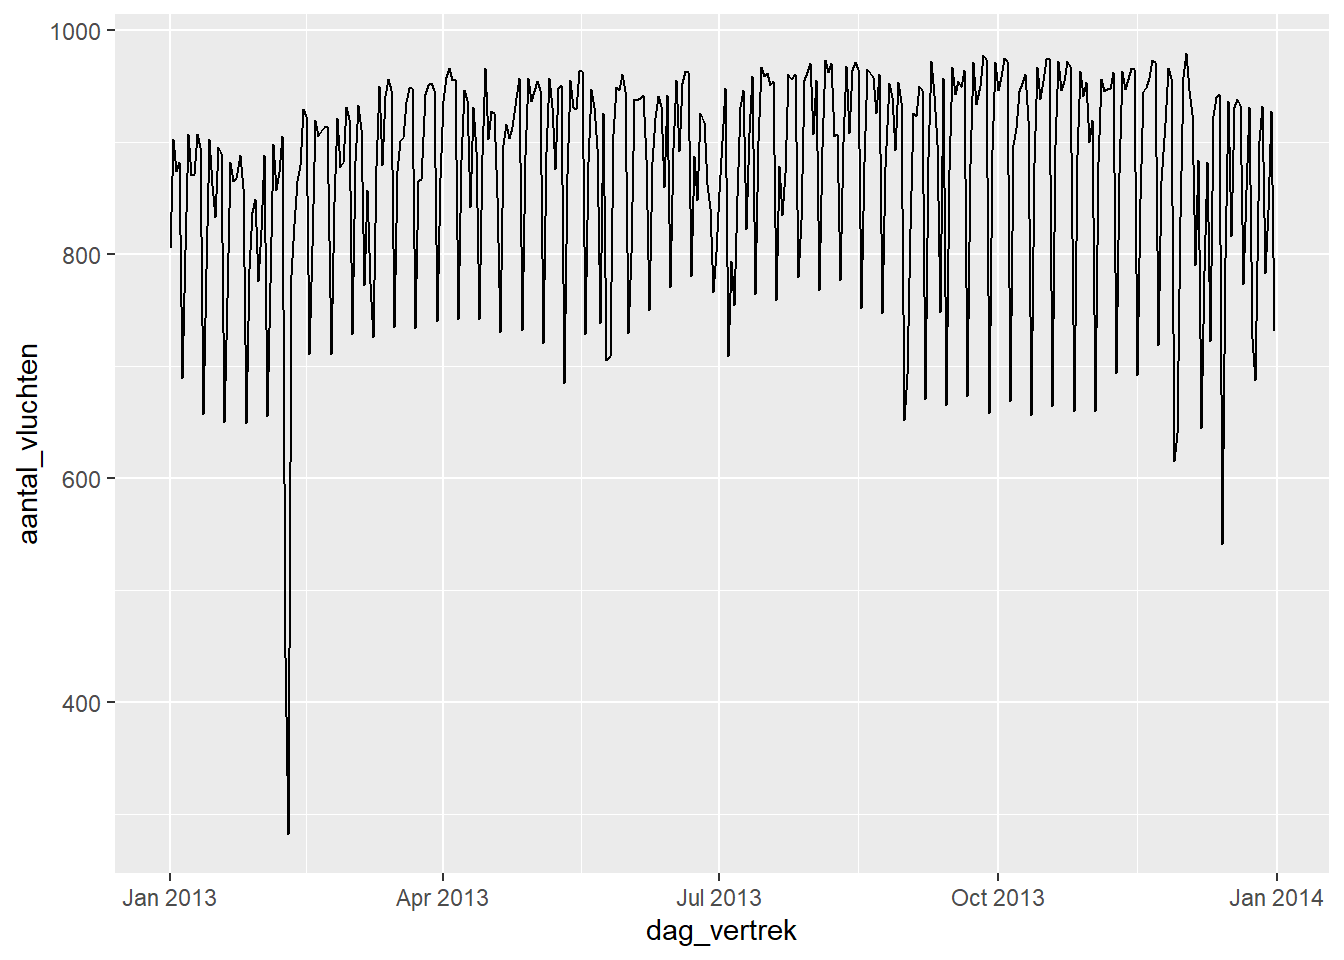
\includegraphics[width=0.49\linewidth]{lecture_notes_edda_files/figure-latex/6.18-1}

\begin{itemize}
\tightlist
\item
  We kunnen een soortgelijke analyse doen voor de gemiddelde vertrekvertraging.
\end{itemize}

\begin{Shaded}
\begin{Highlighting}[]
\NormalTok{df }\OperatorTok
\StringTok{  }\KeywordTok{group_by}\NormalTok{(dag_vertrek) }\OperatorTok
\StringTok{  }\KeywordTok{summarise}\NormalTok{(}\DataTypeTok{gemiddelde_vertrekvertraging =} \KeywordTok{mean}\NormalTok{(vertrek_vertraging)) }\OperatorTok
\StringTok{  }\KeywordTok{ggplot}\NormalTok{(}\KeywordTok{aes}\NormalTok{(}\DataTypeTok{x=}\NormalTok{dag_vertrek, }\DataTypeTok{y=}\NormalTok{gemiddelde_vertrekvertraging)) }\OperatorTok{+}
\StringTok{  }\KeywordTok{geom_line}\NormalTok{()}
\end{Highlighting}
\end{Shaded}

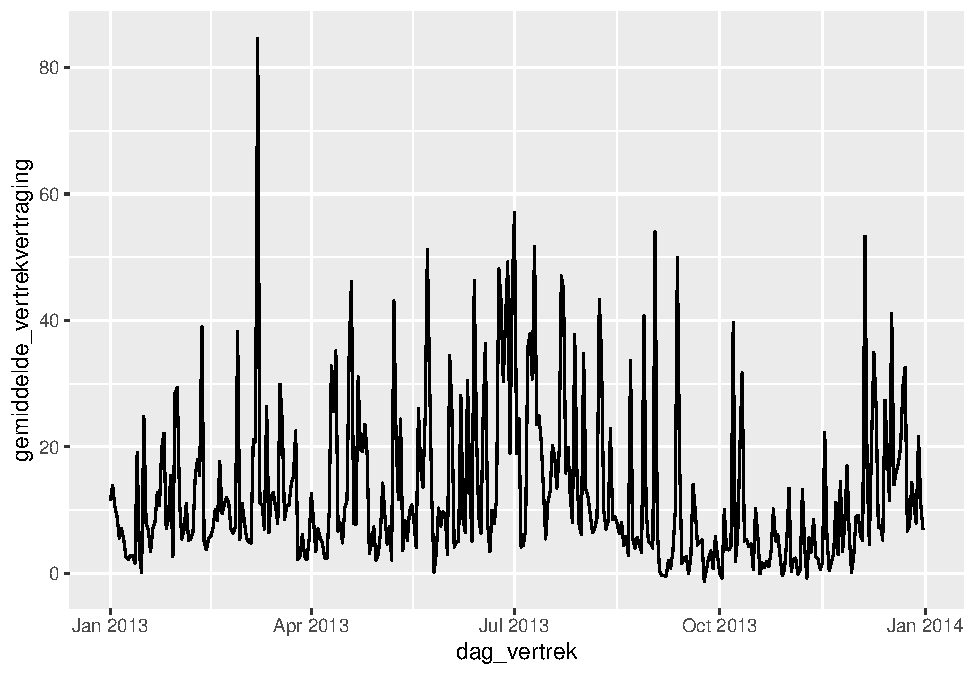
\includegraphics[width=0.49\linewidth]{lecture_notes_edda_files/figure-latex/6.19-1}

\begin{itemize}
\tightlist
\item
  Een volgende stap is vaak om de tijdreekspatronen apart te visualiseren voor de verschillende waarden van een categorische variabele.
\item
  Dit kan op eenvoudige wijze door in onze R-code deze categorische variabele op te nemen in het \emph{group\_by()} gedeelte en vervolgens aparte plots te creëren met behulp van \emph{facet\_wrap()}.
\item
  Laten we de evolutie van het aantal vluchten per dag bijvoorbeeld uitsplitsen per luchthaven.
\item
  Uit onderstaande analyse blijkt dan dat het aantal vluchten vanuit JFK veel minder sterk schommelt dan EWR en LGA. Wel valt op dat alle drie de luchthavens een sterke uitzonderlijke daling kenden in de eerste helft van het jaar.
\end{itemize}

\begin{Shaded}
\begin{Highlighting}[]
\NormalTok{df }\OperatorTok
\StringTok{  }\KeywordTok{group_by}\NormalTok{(dag_vertrek, vertrekluchthaven) }\OperatorTok
\StringTok{  }\KeywordTok{summarise}\NormalTok{(}\DataTypeTok{aantal_vluchten =} \KeywordTok{n}\NormalTok{()) }\OperatorTok
\StringTok{  }\KeywordTok{ggplot}\NormalTok{(}\KeywordTok{aes}\NormalTok{(}\DataTypeTok{x =}\NormalTok{ dag_vertrek, }\DataTypeTok{y =}\NormalTok{ aantal_vluchten, }\DataTypeTok{colour=}\NormalTok{vertrekluchthaven)) }\OperatorTok{+}\StringTok{ }
\StringTok{  }\KeywordTok{geom_line}\NormalTok{() }\OperatorTok{+}\StringTok{ }\KeywordTok{facet_wrap}\NormalTok{(}\OperatorTok{~}\NormalTok{vertrekluchthaven, }\DataTypeTok{ncol =} \DecValTok{1}\NormalTok{)}
\end{Highlighting}
\end{Shaded}

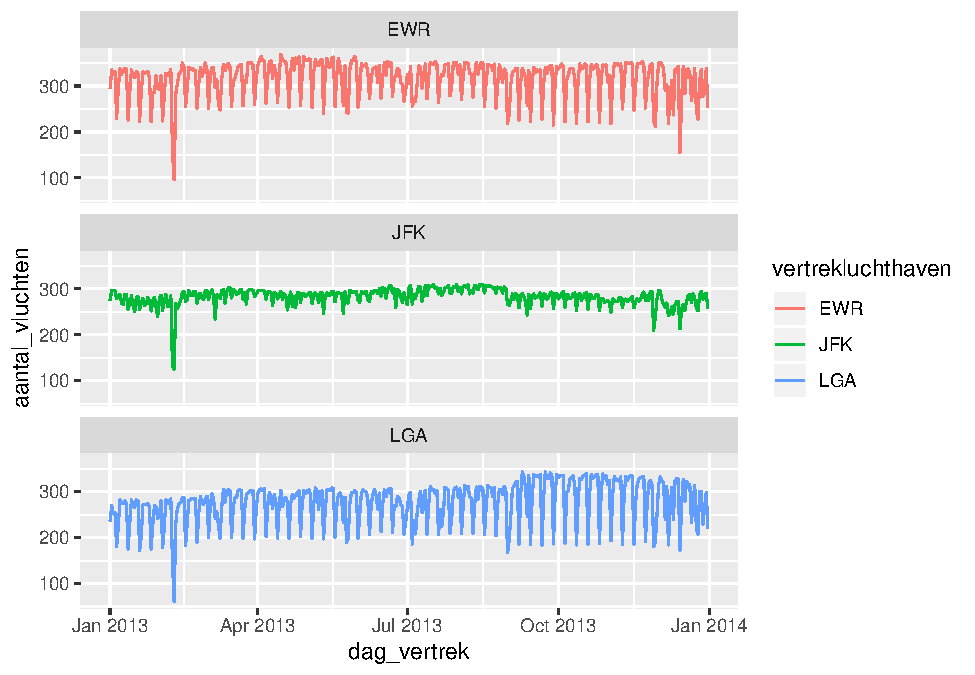
\includegraphics[width=0.49\linewidth]{lecture_notes_edda_files/figure-latex/6.20-1}

\hypertarget{identificeren-van-opmerkelijke-gebeurtenissen-in-een-tijdreeks}{%
\subsubsection{Identificeren van opmerkelijke gebeurtenissen in een tijdreeks}\label{identificeren-van-opmerkelijke-gebeurtenissen-in-een-tijdreeks}}

\begin{itemize}
\tightlist
\item
  In de evolutie van het aantal vluchten valt op dat er een uitzonderlijke daling plaatsvond in de periode tussen januari en april.
\item
  In zulke gevallen is het best te achterhalen wat hier precies de oorzaak is.
\item
  De eerste stap is dan ook het exacte tijdstip te identificeren.
\item
  We kunnen dit doen door de data te filteren op die dagen dat er zeer weinig vluchten zijn.
\end{itemize}

\begin{Shaded}
\begin{Highlighting}[]
\NormalTok{df }\OperatorTok
\StringTok{  }\KeywordTok{group_by}\NormalTok{(dag_vertrek, vertrekluchthaven) }\OperatorTok
\StringTok{  }\KeywordTok{summarise}\NormalTok{(}\DataTypeTok{aantal_vluchten =} \KeywordTok{n}\NormalTok{()) }\OperatorTok
\StringTok{  }\KeywordTok{filter}\NormalTok{(aantal_vluchten }\OperatorTok{<}\StringTok{ }\DecValTok{160}\NormalTok{)}
\end{Highlighting}
\end{Shaded}

\begin{verbatim}
## # A tibble: 7 x 3
## # Groups:   dag_vertrek [3]
##   dag_vertrek         vertrekluchthaven aantal_vluchten
##   <dttm>              <chr>                       <int>
## 1 2013-02-08 00:00:00 EWR                           159
## 2 2013-02-08 00:00:00 JFK                           133
## 3 2013-02-08 00:00:00 LGA                           148
## 4 2013-02-09 00:00:00 EWR                            96
## 5 2013-02-09 00:00:00 JFK                           125
## 6 2013-02-09 00:00:00 LGA                            61
## 7 2013-12-14 00:00:00 EWR                           155
\end{verbatim}

\begin{itemize}
\item
  Uit deze analyse blijkt dat de daling plaatsvond op 8 en 9 februari 2013. Na enig opzoekwerk blijkt dat New York toen geteisterd werd door een hevige sneeuwstorm waardoor zeer veel vluchten geannuleerd moesten worden.
\item
  Omdat dit moment niet representatief is voor een normaal jaar, beslissen we om enkel met de tijdgerelateerde data van maart tot en met december verder te gaan.
\item
  We kunnen de tijdreeks van de nieuwe periode opnieuw visualiseren.
\end{itemize}

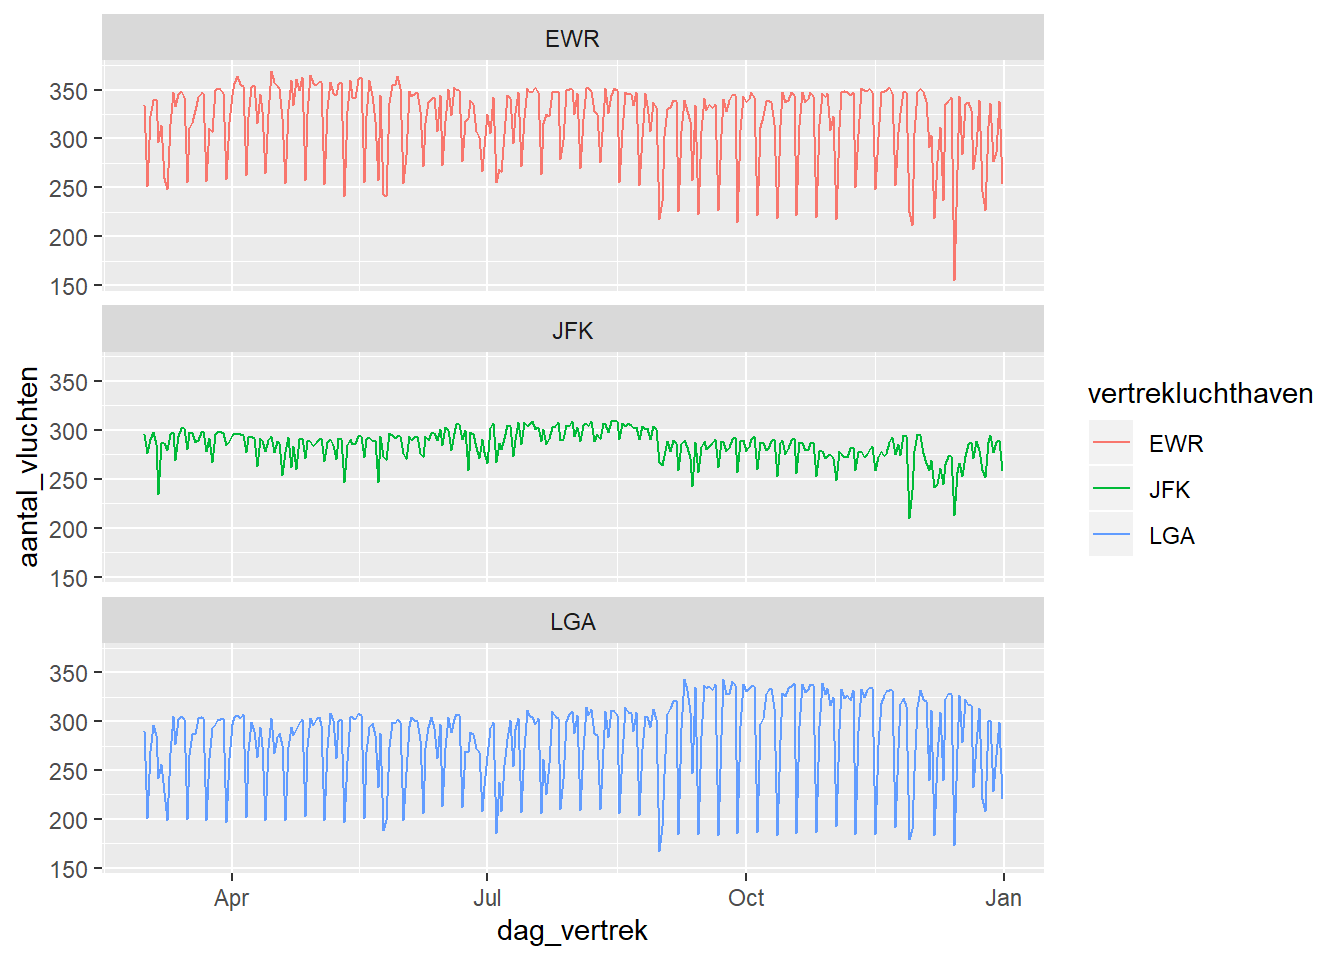
\includegraphics[width=0.49\linewidth]{lecture_notes_edda_files/figure-latex/6.23-1}

\begin{itemize}
\tightlist
\item
  We kunnen verder inzoomen in de data door naar de tijdreekspatronen te kijken per maand en per luchthaven.
\end{itemize}

\begin{Shaded}
\begin{Highlighting}[]
\NormalTok{df_mardec }\OperatorTok
\StringTok{  }\KeywordTok{group_by}\NormalTok{(maanddag_vertrek, maand_vertrek, vertrekluchthaven) }\OperatorTok
\StringTok{  }\KeywordTok{summarise}\NormalTok{(}\DataTypeTok{aantal_vluchten =} \KeywordTok{n}\NormalTok{()) }\OperatorTok
\StringTok{  }\KeywordTok{ggplot}\NormalTok{(}\KeywordTok{aes}\NormalTok{(}\DataTypeTok{x=}\NormalTok{maanddag_vertrek, }\DataTypeTok{y=}\NormalTok{aantal_vluchten, }\DataTypeTok{colour=}\NormalTok{vertrekluchthaven)) }\OperatorTok{+}
\StringTok{  }\KeywordTok{geom_line}\NormalTok{() }\OperatorTok{+}\StringTok{ }\KeywordTok{facet_grid}\NormalTok{(maand_vertrek }\OperatorTok{~}\StringTok{ }\NormalTok{vertrekluchthaven)}
\end{Highlighting}
\end{Shaded}

\includegraphics[width=0.49\linewidth]{lecture_notes_edda_files/figure-latex/6.24-1}

\hypertarget{referenties-4}{%
\section{Referenties}\label{referenties-4}}

\begin{enumerate}
\def\labelenumi{\arabic{enumi}.}
\tightlist
\item
  \href{http://r4ds.had.co.nz/}{`R for Data Science' van Grolemund en Wickham}
\end{enumerate}

\hypertarget{tidy-data}{%
\chapter{Tidy Data}\label{tidy-data}}

\hypertarget{inleiding-1}{%
\section{Inleiding}\label{inleiding-1}}

\begin{itemize}
\tightlist
\item
  In werkelijkheid komt data niet altijd in het geschikte formaat om de gewenste analyses op uit te voeren.

  \begin{itemize}
  \tightlist
  \item
    Vaak is data verspreid over meerdere datasets en moeten we hier 1 dataframe van maken voor onze analyses.
  \item
    Soms stelt een rij niet de observatie voor die willen bestuderen (bv: één rij stelt de gegevens van één auto betrokken in een ongeval voor, terwijl we willen dat iedere rij een ongeval voorstelt met de gegevens van alle betrokken voertuigen).
  \end{itemize}
\item
  Het manipuleren van de data opdat het in het juiste formaat staat, wordt ook wel de creatie van `tidy data' genoemd.
\item
  \textbf{Bestudeer secties 12.1 tot en met 12.4 en 12.6 in `R for Data Science' van Grolemund en Wickham!}
\item
  \textbf{Bestudeer hoofdstuk 13 in `R for Data Science' van Grolemund en Wickham!}
\end{itemize}

\hypertarget{case-nyc-vluchten-2013-3}{%
\section{Case: NYC Vluchten 2013}\label{case-nyc-vluchten-2013-3}}

\hypertarget{datasets-samenvoegen}{%
\subsection{Datasets samenvoegen}\label{datasets-samenvoegen}}

\begin{itemize}
\tightlist
\item
  We vertrekken van een dataset met vluchten opgestegen vanuit NYC in 2013. Hieronder een overzicht van de variabelen in de dataset.
\end{itemize}

\begin{verbatim}
## Observations: 319,809
## Variables: 13
## $ id                  <int> 1, 2, 3, 4, 5, 6, 7, 8, 9, 10, 11, 12, 13,...
## $ vertrekluchthaven   <chr> "EWR", "LGA", "JFK", "LGA", "EWR", "EWR", ...
## $ aankomstluchthaven  <chr> "George Bush Intercontinental", "George Bu...
## $ maatschappij        <chr> "United Air Lines Inc.", "United Air Lines...
## $ tijdstip_aankomst   <dttm> 2013-01-01 08:30:00, 2013-01-01 08:50:00,...
## $ vertrek_vertraging  <dbl> 2, 4, 2, -6, -4, -5, -3, -3, -2, -2, -2, -...
## $ aankomst_vertraging <dbl> 11, 20, 33, -25, 12, 19, -14, -8, 8, -2, -...
## $ afstand             <dbl> 1400, 1416, 1089, 762, 719, 1065, 229, 944...
## $ tijdstip_vertrek    <dttm> 2013-01-01 05:17:00, 2013-01-01 05:33:00,...
## $ weekdag_vertrek     <ord> Tue, Tue, Tue, Tue, Tue, Tue, Tue, Tue, Tu...
## $ week_vertrek        <dbl> 1, 1, 1, 1, 1, 1, 1, 1, 1, 1, 1, 1, 1, 1, ...
## $ maand_vertrek       <dbl> 1, 1, 1, 1, 1, 1, 1, 1, 1, 1, 1, 1, 1, 1, ...
## $ maanddag_vertrek    <int> 1, 1, 1, 1, 1, 1, 1, 1, 1, 1, 1, 1, 1, 1, ...
\end{verbatim}

\begin{itemize}
\tightlist
\item
  We beschikken nu ook over een tweede dataset met de gegevens van de luchthavens. Hieronder een overzicht van de variabelen in deze dataset.
\end{itemize}

\begin{verbatim}
## Observations: 1,458
## Variables: 8
## $ faa   <chr> "04G", "06A", "06C", "06N", "09J", "0A9", "0G6", "0G7", ...
## $ name  <chr> "Lansdowne Airport", "Moton Field Municipal Airport", "S...
## $ lat   <dbl> 41.13047, 32.46057, 41.98934, 41.43191, 31.07447, 36.371...
## $ lon   <dbl> -80.61958, -85.68003, -88.10124, -74.39156, -81.42778, -...
## $ alt   <dbl> 1044, 264, 801, 523, 11, 1593, 730, 492, 1000, 108, 409,...
## $ tz    <dbl> -5, -6, -6, -5, -5, -5, -5, -5, -5, -8, -5, -6, -5, -5, ...
## $ dst   <chr> "A", "A", "A", "A", "A", "A", "A", "A", "U", "A", "A", "...
## $ tzone <chr> "America/New_York", "America/Chicago", "America/Chicago"...
\end{verbatim}

\begin{itemize}
\tightlist
\item
  Als we deze datasets vergelijken zien we een mogelijke relatie tussen beiden.

  \begin{itemize}
  \tightlist
  \item
    In de oorspronkelijke dataset stelt iedere rij een vlucht voor en wordt de vertrekluchthaven voorgesteld door een 3-letterige code.
  \item
    In de airports-dataset stelt iedere rij een luchthaven voor en vinden we een 3-letterige code terug in de kolom `faa'.
  \end{itemize}
\item
  We willen nu graag deze twee datasets aan elkaar koppelen door de gegevens van de vertrekluchthavens uit de airports-dataset te halen en toe te voegen aan iedere vlucht.
\item
  Alvorens we dit kunnen doen, moeten we eerst controleren of de faa-code in de airports-dataset uniek is.

  \begin{itemize}
  \tightlist
  \item
    Dit is een essentiële vereiste om de gegevens van de airports-dataset te kunnen toevoegen aan de oorspronkelijke dataset.
  \item
    Indien er bijvoorbeeld 2 luchthavens in de airports-dataset zouden zitten met faa-code `EWR', dan zou R niet kunnen achterhalen van welke luchthaven de gegevens moeten worden toegevoegd aan de vluchten met als vertrekluchthaven `EWR'.
  \item
    In zulke gevallen gaat R de vlucht dupliceren en iedere kopie (van de vlucht) koppelen aan een andere luchthaven uit de airports-dataset met faa-code EWR.
  \end{itemize}
\end{itemize}

\begin{verbatim}
## # A tibble: 0 x 2
## # ... with 2 variables: faa <chr>, n <int>
\end{verbatim}

\begin{itemize}
\tightlist
\item
  Uit bovenstaande analyse blijkt dat er geen twee rijen zijn in de airports-dataset met dezelfde faa-code.
\item
  We kunnen nu de gegevens van de airports-dataset toevoegen aan het oorspronkelijk dataframe. We doen dit met behulp van een \emph{left\_join()} en geven aan via welke variabelen de link gelegd moet worden.
\end{itemize}

\begin{verbatim}
## Observations: 319,809
## Variables: 20
## $ id                  <int> 1, 2, 3, 4, 5, 6, 7, 8, 9, 10, 11, 12, 13,...
## $ vertrekluchthaven   <chr> "EWR", "LGA", "JFK", "LGA", "EWR", "EWR", ...
## $ aankomstluchthaven  <chr> "George Bush Intercontinental", "George Bu...
## $ maatschappij        <chr> "United Air Lines Inc.", "United Air Lines...
## $ tijdstip_aankomst   <dttm> 2013-01-01 08:30:00, 2013-01-01 08:50:00,...
## $ vertrek_vertraging  <dbl> 2, 4, 2, -6, -4, -5, -3, -3, -2, -2, -2, -...
## $ aankomst_vertraging <dbl> 11, 20, 33, -25, 12, 19, -14, -8, 8, -2, -...
## $ afstand             <dbl> 1400, 1416, 1089, 762, 719, 1065, 229, 944...
## $ tijdstip_vertrek    <dttm> 2013-01-01 05:17:00, 2013-01-01 05:33:00,...
## $ weekdag_vertrek     <ord> Tue, Tue, Tue, Tue, Tue, Tue, Tue, Tue, Tu...
## $ week_vertrek        <dbl> 1, 1, 1, 1, 1, 1, 1, 1, 1, 1, 1, 1, 1, 1, ...
## $ maand_vertrek       <dbl> 1, 1, 1, 1, 1, 1, 1, 1, 1, 1, 1, 1, 1, 1, ...
## $ maanddag_vertrek    <int> 1, 1, 1, 1, 1, 1, 1, 1, 1, 1, 1, 1, 1, 1, ...
## $ name                <chr> "Newark Liberty Intl", "La Guardia", "John...
## $ lat                 <dbl> 40.69250, 40.77725, 40.63975, 40.77725, 40...
## $ lon                 <dbl> -74.16867, -73.87261, -73.77893, -73.87261...
## $ alt                 <dbl> 18, 22, 13, 22, 18, 18, 22, 13, 22, 13, 13...
## $ tz                  <dbl> -5, -5, -5, -5, -5, -5, -5, -5, -5, -5, -5...
## $ dst                 <chr> "A", "A", "A", "A", "A", "A", "A", "A", "A...
## $ tzone               <chr> "America/New_York", "America/New_York", "A...
\end{verbatim}

\begin{itemize}
\tightlist
\item
  Bovenstaande output laat zien dat 7 kolommen zijn toegevoegd aan de oorspronkelijke dataset.
\item
  Merk op dat de faa-kolom van het airports-dataframe niet is toegevoegd. Dit is niet nodig aangezien we in de join-functie hadden aangegeven dat deze kolom overeenkwam met de kolom vertrekluchthaven uit de oorspronkelijke dataset.
\item
  Controleer ook altijd of het aantal observaties niet gewijzigd is, daar dit vaak wijst op een fout in de join. In dit geval is het aantal observaties niet veranderd.
\item
  In een volgende stap verwijderen we een aantal kolommen die we verder niet nodig gaan hebben en veranderen we de kolom `name' in `vertrekluchthaven'. Zoals je in het resultaat kan zien bevat onze nieuwe dataset nu de volledige naam van de vertrekluchthaven en niet enkel de faa-code.
\end{itemize}

\begin{verbatim}
## Observations: 319,809
## Variables: 13
## $ id                  <int> 1, 2, 3, 4, 5, 6, 7, 8, 9, 10, 11, 12, 13,...
## $ aankomstluchthaven  <chr> "George Bush Intercontinental", "George Bu...
## $ maatschappij        <chr> "United Air Lines Inc.", "United Air Lines...
## $ tijdstip_aankomst   <dttm> 2013-01-01 08:30:00, 2013-01-01 08:50:00,...
## $ vertrek_vertraging  <dbl> 2, 4, 2, -6, -4, -5, -3, -3, -2, -2, -2, -...
## $ aankomst_vertraging <dbl> 11, 20, 33, -25, 12, 19, -14, -8, 8, -2, -...
## $ afstand             <dbl> 1400, 1416, 1089, 762, 719, 1065, 229, 944...
## $ tijdstip_vertrek    <dttm> 2013-01-01 05:17:00, 2013-01-01 05:33:00,...
## $ weekdag_vertrek     <ord> Tue, Tue, Tue, Tue, Tue, Tue, Tue, Tue, Tu...
## $ week_vertrek        <dbl> 1, 1, 1, 1, 1, 1, 1, 1, 1, 1, 1, 1, 1, 1, ...
## $ maand_vertrek       <dbl> 1, 1, 1, 1, 1, 1, 1, 1, 1, 1, 1, 1, 1, 1, ...
## $ maanddag_vertrek    <int> 1, 1, 1, 1, 1, 1, 1, 1, 1, 1, 1, 1, 1, 1, ...
## $ vertrekluchthaven   <chr> "Newark Liberty Intl", "La Guardia", "John...
\end{verbatim}

\hypertarget{data-in-een-lang-formaat-plaatsen-voor-visuele-analyses}{%
\section{Data in een lang formaat plaatsen (voor visuele analyses)}\label{data-in-een-lang-formaat-plaatsen-voor-visuele-analyses}}

\begin{itemize}
\tightlist
\item
  Bij een bivariate visualisatie heb je steeds het basisprincipe dat je de relatie tussen twee variabelen wenst weer te geven.
\item
  Bij een multivariate visualisatie ga je vaak weergeven hoe deze relatie verandert in functie van een derde variabele.
\item
  Deze derde variabele is vaak categorisch en de verschillende categorieën stellen hierbij groeperingen van de observaties voor waarvoor je de relatie tussen X en Y wenst weer te geven.

  \begin{itemize}
  \tightlist
  \item
    Je wil bijvoorbeeld initieel de relatie tussen weekdag en afstand van de vluchten weergeven. Hiervoor kan je een bivariate plot maken waarbij X categorisch is en Y continu. Een mogelijkheid hiervoor is een boxplot.
  \item
    In een volgende stap kan je de relatie tussen afstand en weekdag opsplitsen per luchthaven. Je wil dus weten hoe deze relatie verschilt tussen diverse luchthavens. Hiervoor gebruik je de categorische variabele `vertrekluchthaven' en kan je bijvoorbeeld de kleur van de boxplot koppelen aan de vertrekluchthaven of aparte `facets' maken voor iedere luchthaven.
  \item
    Hieronder zie je de bijhorende plots.
  \end{itemize}
\end{itemize}

\includegraphics[width=0.49\linewidth]{lecture_notes_edda_files/figure-latex/7.7-1}

\includegraphics[width=0.49\linewidth]{lecture_notes_edda_files/figure-latex/7.8-1}

\begin{itemize}
\tightlist
\item
  Stel nu dat je het effect wenst te weten van de weekdag van vertrek op de vertraging van een vlucht, maar je wil hierbij onderscheid maken tussen vertrek- en aankomstvertraging.
\item
  Volgens bovenstaande aanpak zou je dan een Y-variabele moeten hebben die de vertraging meet en een Z-variabele die het type van vertraging aangeeft (aankomst of vertrek).
\item
  Onze dataset is echter anders opgebouwd. In de beschikbare data is de vertraging van een vlucht opgeslagen met behulp van twee aparte variabelen, namelijk vertrek- en aankomstvertraging. Dit blijkt uit onderstaande tabel.
\end{itemize}

\begin{verbatim}
## # A tibble: 319,809 x 5
##       id vertrekluchthav~ vertrek_vertrag~ aankomst_vertra~ weekdag_vertrek
##    <int> <chr>                       <dbl>            <dbl> <ord>          
##  1     1 Newark Liberty ~                2               11 Tue            
##  2     2 La Guardia                      4               20 Tue            
##  3     3 John F Kennedy ~                2               33 Tue            
##  4     4 La Guardia                     -6              -25 Tue            
##  5     5 Newark Liberty ~               -4               12 Tue            
##  6     6 Newark Liberty ~               -5               19 Tue            
##  7     7 La Guardia                     -3              -14 Tue            
##  8     8 John F Kennedy ~               -3               -8 Tue            
##  9     9 La Guardia                     -2                8 Tue            
## 10    10 John F Kennedy ~               -2               -2 Tue            
## # ... with 319,799 more rows
\end{verbatim}

\begin{itemize}
\tightlist
\item
  We moeten de data dus omzetten zodat het type vertraging niet gecodeerd wordt als aparte variabelen, maar door middel van 1 categorische variabele.
\item
  Hiervoor kunnen we de \emph{gather()} functie hanteren. Deze functie zal een set van variabelen (in dit geval `vertrek\_vertraging' en `aankomst\_vertraging') transformeren naar 2 variabelen, namelijk een key-variabele en een value-variabele.

  \begin{itemize}
  \tightlist
  \item
    De key-variabele is een categorische variabele en de categorieën komen overeen met de variabelenamen in onze set van variabelen die we wensen te transformeren. In ons geval zijn dit dus de categorieën `vertrek\_vertraging' en `aankomst\_vertraging'.
  \item
    De value-variabele bevat de bijhorende waarde uit de oorspronkelijke dataset.
  \end{itemize}
\item
  De \emph{gather()} functie bestaat uit 3 delen.

  \begin{itemize}
  \tightlist
  \item
    Eerst vermeld je alle variabelen die je wenst te vervangen.
  \item
    Vervolgens geef je de naam van de nieuwe key-variabele.
  \item
    Tenslotte geef je de naam van de nieuwe value-variabele.
  \end{itemize}
\end{itemize}

\begin{verbatim}
## # A tibble: 639,618 x 5
##       id vertrekluchthaven   weekdag_vertrek type_vertraging     vertraging
##    <int> <chr>               <ord>           <chr>                    <dbl>
##  1     1 Newark Liberty Intl Tue             vertrek_vertraging           2
##  2     1 Newark Liberty Intl Tue             aankomst_vertraging         11
##  3     2 La Guardia          Tue             vertrek_vertraging           4
##  4     2 La Guardia          Tue             aankomst_vertraging         20
##  5     3 John F Kennedy Intl Tue             vertrek_vertraging           2
##  6     3 John F Kennedy Intl Tue             aankomst_vertraging         33
##  7     4 La Guardia          Tue             vertrek_vertraging          -6
##  8     4 La Guardia          Tue             aankomst_vertraging        -25
##  9     5 Newark Liberty Intl Tue             vertrek_vertraging          -4
## 10     5 Newark Liberty Intl Tue             aankomst_vertraging         12
## # ... with 639,608 more rows
\end{verbatim}

\begin{itemize}
\tightlist
\item
  Merk op dat het aantal rijen nu verdubbeld is. Dit komt omdat je nu voor zowel vertrek- als aankomstvertraging een aparte rij hebt gecreëerd.

  \begin{itemize}
  \tightlist
  \item
    Hierdoor krijg je een andere definitie van de observatie die in een rij staat. In de oorspronkelijke dataset was iedere rij (observatie) een vlucht vanuit NYC in 2013. In de nieuwe dataset stelt iedere rij het vertrek of de aankomst van een vlucht vanuit NYC in 2013 voor!
  \end{itemize}
\item
  Indien je dus de \emph{gather()} functie hanteert gaat het aantal rijen toenemen. Het aantal kolommen zal afnemen indien de variabelenset, die je wenst te transformeren, uit meer dan 2 variabelen bestaat.
\item
  Hierdoor krijg je een dataset die minder breed is en vooral langer. Daarom wordt dit het lange formaat genoemd.
\item
  Data in een lang formaat zijn voornamelijk nuttig om visualisaties te realiseren met ggplot.
\item
  Met dit lange formaat kunnen we de relatie tussen weekdag van vertrek en de vertraging, uitgesplitst volgens vertrek- of aankomstvertraging, visualiseren.
\end{itemize}

\includegraphics[width=0.49\linewidth]{lecture_notes_edda_files/figure-latex/7.11-1}

\begin{itemize}
\tightlist
\item
  Indien we de relatie tussen we weekdag en de gemiddelde vertraging, uitgesplitst volgens vertragingtype, wensen te visualiseren, moeten we eerst de gemiddelde vertraging berekenen.
\end{itemize}

\begin{verbatim}
## # A tibble: 42 x 4
## # Groups:   vertrekluchthaven, type_vertraging [6]
##    vertrekluchthaven   type_vertraging     weekdag_vertrek gem_vertraging
##    <chr>               <chr>               <ord>                    <dbl>
##  1 John F Kennedy Intl aankomst_vertraging Sun                       6.39
##  2 John F Kennedy Intl aankomst_vertraging Mon                       7.99
##  3 John F Kennedy Intl aankomst_vertraging Tue                       3.34
##  4 John F Kennedy Intl aankomst_vertraging Wed                       5.86
##  5 John F Kennedy Intl aankomst_vertraging Thu                       7.56
##  6 John F Kennedy Intl aankomst_vertraging Fri                       6.49
##  7 John F Kennedy Intl aankomst_vertraging Sat                       1.96
##  8 John F Kennedy Intl vertrek_vertraging  Sun                      11.7 
##  9 John F Kennedy Intl vertrek_vertraging  Mon                      14.7 
## 10 John F Kennedy Intl vertrek_vertraging  Tue                      10.5 
## # ... with 32 more rows
\end{verbatim}

\includegraphics[width=0.49\linewidth]{lecture_notes_edda_files/figure-latex/7.13-1}

\hypertarget{data-in-een-breed-formaat-plaatsen-voor-overzichtelijke-tabellen}{%
\section{Data in een breed formaat plaatsen (voor overzichtelijke tabellen)}\label{data-in-een-breed-formaat-plaatsen-voor-overzichtelijke-tabellen}}

\begin{itemize}
\tightlist
\item
  Voor de laatste visualisatie hebben we een dataset gecreëerd met gemiddelde vertragingen per vertrekluchthaven, weekdag van vertrek en type vertraging.
\end{itemize}

\begin{table}[t]

\caption{\label{tab:7-14b}Gemiddelde vertraging (lang formaat)}
\centering
\fontsize{10}{12}\selectfont
\begin{tabular}{lllr}
\toprule
weekdag\_vertrek & vertrekluchthaven & type\_vertraging & gem\_vertraging\\
\midrule
Sun & John F Kennedy Intl & aankomst\_vertraging & 6.39\\
Sun & John F Kennedy Intl & vertrek\_vertraging & 11.70\\
Sun & La Guardia & aankomst\_vertraging & 0.15\\
Sun & La Guardia & vertrek\_vertraging & 8.33\\
Sun & Newark Liberty Intl & aankomst\_vertraging & 7.44\\
\addlinespace
Sun & Newark Liberty Intl & vertrek\_vertraging & 14.01\\
Mon & John F Kennedy Intl & aankomst\_vertraging & 7.99\\
Mon & John F Kennedy Intl & vertrek\_vertraging & 14.74\\
Mon & La Guardia & aankomst\_vertraging & 9.58\\
Mon & La Guardia & vertrek\_vertraging & 12.86\\
\addlinespace
Mon & Newark Liberty Intl & aankomst\_vertraging & 11.67\\
Mon & Newark Liberty Intl & vertrek\_vertraging & 16.73\\
Tue & John F Kennedy Intl & aankomst\_vertraging & 3.34\\
Tue & John F Kennedy Intl & vertrek\_vertraging & 10.47\\
Tue & La Guardia & aankomst\_vertraging & 5.60\\
\addlinespace
Tue & La Guardia & vertrek\_vertraging & 8.63\\
Tue & Newark Liberty Intl & aankomst\_vertraging & 7.15\\
Tue & Newark Liberty Intl & vertrek\_vertraging & 12.57\\
Wed & John F Kennedy Intl & aankomst\_vertraging & 5.86\\
Wed & John F Kennedy Intl & vertrek\_vertraging & 11.71\\
\addlinespace
Wed & La Guardia & aankomst\_vertraging & 6.23\\
Wed & La Guardia & vertrek\_vertraging & 9.15\\
Wed & Newark Liberty Intl & aankomst\_vertraging & 9.02\\
Wed & Newark Liberty Intl & vertrek\_vertraging & 13.95\\
Thu & John F Kennedy Intl & aankomst\_vertraging & 7.56\\
\addlinespace
Thu & John F Kennedy Intl & vertrek\_vertraging & 13.65\\
Thu & La Guardia & aankomst\_vertraging & 11.89\\
Thu & La Guardia & vertrek\_vertraging & 14.10\\
Thu & Newark Liberty Intl & aankomst\_vertraging & 15.60\\
Thu & Newark Liberty Intl & vertrek\_vertraging & 20.10\\
\addlinespace
Fri & John F Kennedy Intl & aankomst\_vertraging & 6.49\\
Fri & John F Kennedy Intl & vertrek\_vertraging & 12.76\\
Fri & La Guardia & aankomst\_vertraging & 7.97\\
Fri & La Guardia & vertrek\_vertraging & 12.45\\
Fri & Newark Liberty Intl & aankomst\_vertraging & 12.55\\
\addlinespace
Fri & Newark Liberty Intl & vertrek\_vertraging & 18.49\\
Sat & John F Kennedy Intl & aankomst\_vertraging & 1.96\\
Sat & John F Kennedy Intl & vertrek\_vertraging & 9.97\\
Sat & La Guardia & aankomst\_vertraging & -5.44\\
Sat & La Guardia & vertrek\_vertraging & 4.19\\
\addlinespace
Sat & Newark Liberty Intl & aankomst\_vertraging & -2.22\\
Sat & Newark Liberty Intl & vertrek\_vertraging & 7.63\\
\bottomrule
\end{tabular}
\end{table}

\begin{itemize}
\tightlist
\item
  Om snel verbanden te zoeken en te evalueren is dit formaat niet erg handig. Voor zulke situaties kan je best voor een breed formaat opteren.

  \begin{itemize}
  \tightlist
  \item
    Hierbij moet je 2 variabelen selecteren: de key-variabele en de value-variabele.
  \item
    De key-variabele is altijd een categorische variabele en de value-variabele kan zowel categorisch als continu zijn.
  \item
    Voor ieder level van de categorische key-variabele zal er een aparte kolom aangemaakt worden.
  \end{itemize}
\item
  Je kan een dataset van lang naar breed formaat omzetten met behulp van de \emph{spread()} functie.
\end{itemize}

\begin{Shaded}
\begin{Highlighting}[]
\NormalTok{df_long_summary }\OperatorTok
\StringTok{  }\KeywordTok{spread}\NormalTok{(}\DataTypeTok{key=}\NormalTok{weekdag_vertrek, }\DataTypeTok{value=}\NormalTok{gem_vertraging) }\OperatorTok
\StringTok{  }\KeywordTok{arrange}\NormalTok{(vertrekluchthaven, type_vertraging)}
\end{Highlighting}
\end{Shaded}

\begin{table}[t]

\caption{\label{tab:7-15b}Gemiddelde vertraging (breed formaat).}
\centering
\fontsize{10}{12}\selectfont
\begin{tabular}{llrrrrrrr}
\toprule
vertrekluchthaven & type\_vertraging & Sun & Mon & Tue & Wed & Thu & Fri & Sat\\
\midrule
John F Kennedy Intl & aankomst\_vertraging & 6.39 & 7.99 & 3.34 & 5.86 & 7.56 & 6.49 & 1.96\\
John F Kennedy Intl & vertrek\_vertraging & 11.70 & 14.74 & 10.47 & 11.71 & 13.65 & 12.76 & 9.97\\
La Guardia & aankomst\_vertraging & 0.15 & 9.58 & 5.60 & 6.23 & 11.89 & 7.97 & -5.44\\
La Guardia & vertrek\_vertraging & 8.33 & 12.86 & 8.63 & 9.15 & 14.10 & 12.45 & 4.19\\
Newark Liberty Intl & aankomst\_vertraging & 7.44 & 11.67 & 7.15 & 9.02 & 15.60 & 12.55 & -2.22\\
\addlinespace
Newark Liberty Intl & vertrek\_vertraging & 14.01 & 16.73 & 12.57 & 13.95 & 20.10 & 18.49 & 7.63\\
\bottomrule
\end{tabular}
\end{table}

\hypertarget{referenties-5}{%
\section{Referenties}\label{referenties-5}}

\begin{enumerate}
\def\labelenumi{\arabic{enumi}.}
\tightlist
\item
  \href{http://r4ds.had.co.nz/}{`R for Data Science' van Grolemund en Wickham}
\end{enumerate}

\hypertarget{inleiding-2}{%
\chapter{Inleiding}\label{inleiding-2}}

Deze tutorial bestaat uit 2 delen, een introductie tot GGplot en een beschrijving van de creatie van een beschrijvend data-analyserapport. Deze tutorial is origineel geschreven als een RMarkdown document.

\#GGPlot

We beginnen met een korte inleiding tot GGplot waarin we trachten de principes uit te leggen. We zullen GGPlot verder uitdiepen in de beschrijvende data analyse.

GGplot is een soort grammatica waarmee je een grafiek kan opdelen in verschillende elementen die onafhankelijk zijn van elkaar. De belangrijkste elementen van deze grammatica zijn:

\begin{itemize}
\tightlist
\item
  Data
\item
  Geometrische objecten (geoms)
\item
  Esthetische kenmerken (van geometrische objecten) (aesthetics)
\item
  Lagen (layers)
\end{itemize}

Alles begint met \emph{data}. Dit bevat de informatie die je wilt visualiseren en ggplot verwacht deze data als een data.frame object. Door het kiezen van een specifiek \emph{geometrisch object} bepaal je hoe je de data wenst te visualeren, bijvoorbeeld als een punt (point), een lijn (line), een boxplot (boxplot) of als balken (bar).

Ieder geometrisch object heeft een aantal \emph{esthetische kenmerken}, zoals bijvoorbeeld de kleur (color), de grootte (size) of de vorm (shape). Twee esthetische kenmerken die misschien niet onmiddellijk als esthetisch worden beschouwd, maar wel zeer belangrijk zijn, zijn de x- en y-coördinaat.

GGplot linkt de \emph{data} met het \emph{geometrisch object} door kolommen/variabelen te mappen aan de esthetische kenmerken van een geometrisch object. Je gaat tegen GGplot zeggen welke 2 variabelen (= kolommen in je data.frame) de x- en y-coördinaat van iedere observatie (= rij in data.frame) voorstellen.

Iedere mapping tussen data en het geometrisch object vormt een \emph{layer}. Een layer kan je zien als een transparant blad, dat bovenop het assenstelsel gelegd wordt, en waarop een `grafiek' staat. Een volledige grafieke (plot) kan uit meerdere layers bestaan die boven op elkaar liggen.

Laten we deze principes eens illustreren met een concreet voorbeeld. Hiervoor laden we de mpg data set die standaard in ggplot2 zit.

\begin{verbatim}
## Observations: 234
## Variables: 11
## $ manufacturer <chr> "audi", "audi", "audi", "audi", "audi", "audi", "...
## $ model        <chr> "a4", "a4", "a4", "a4", "a4", "a4", "a4", "a4 qua...
## $ displ        <dbl> 1.8, 1.8, 2.0, 2.0, 2.8, 2.8, 3.1, 1.8, 1.8, 2.0,...
## $ year         <int> 1999, 1999, 2008, 2008, 1999, 1999, 2008, 1999, 1...
## $ cyl          <int> 4, 4, 4, 4, 6, 6, 6, 4, 4, 4, 4, 6, 6, 6, 6, 6, 6...
## $ trans        <chr> "auto(l5)", "manual(m5)", "manual(m6)", "auto(av)...
## $ drv          <chr> "f", "f", "f", "f", "f", "f", "f", "4", "4", "4",...
## $ cty          <int> 18, 21, 20, 21, 16, 18, 18, 18, 16, 20, 19, 15, 1...
## $ hwy          <int> 29, 29, 31, 30, 26, 26, 27, 26, 25, 28, 27, 25, 2...
## $ fl           <chr> "p", "p", "p", "p", "p", "p", "p", "p", "p", "p",...
## $ class        <chr> "compact", "compact", "compact", "compact", "comp...
\end{verbatim}

De variabele `displ' stelt de cilinderinhoud voor (in liters), terwijl de variabelen `cty' en `hwy' het aantal kilometers per gallon voorstellen in respectievelijk een stedelijke omgeving of op de autostrade. Iedere observatie stelt een automodel voor in de periode 1999 en 2008.

Veronderstel nu dat we het verband willen visualiseren tussen de cilinderinhoud en het verbruik in de stand. Een eerste mogelijkheid is dit verband te visualiseren als punten waarbij de x-coördinaat overeenkomt met de cilinderinhoud (`displ') en de y-coördinaat overeenkomt met het stadsverbruik (`cty'). De ggplot code ziet er dan als volgt uit:

\includegraphics[width=0.49\linewidth]{lecture_notes_edda_files/figure-latex/unnamed-chunk-7-1}

Zoals je ziet wordt er een layer gecreëerd waarbij:

\begin{itemize}
\tightlist
\item
  we aangeven dat mpg het te gebruiken data.frame is,
\item
  de mapping gebeurt door de esthetische kenmerken `x' en `y' te koppelen aan respectievelijk de kolommen `displ' en `cty' en
\item
  de observaties weergegeven dienen te worden als punten.
\end{itemize}

Laten we nog een ander esthetisch kenmerk van het punten-object mappen, nl. de kleur. We willen nu dat de kleur varieert naargelang de auto voorwiel-, achterwiel- of vierwiel-aandrijving heeft.

\includegraphics[width=0.49\linewidth]{lecture_notes_edda_files/figure-latex/unnamed-chunk-8-1}

We kunnen esthetische kenmerken niet enkel mappen aan variabelen uit data (waardoor het esthetisch kenmerk gaat variëren naargelang de waarde van de variabele), maar ook vastleggen op een constante waarde (dit wordt dan ook `setten' genoemd ipv `mappen'). Laten we de kleur bijvoorbeeld vastleggen op een blauwe kleur. Merk op dat het instellen van de kleur nu buiten de aes()-functie gebeurt aangezien dit geen mapping is!

\includegraphics[width=0.49\linewidth]{lecture_notes_edda_files/figure-latex/unnamed-chunk-9-1}

Tot dusver bestond iedere grafiek uit slechts 1 laag (layer), maar laten we nu een tweede laag aan de grafiek toevoegen die ook het verbruik op de autostrade weergeeft. We doen dit door een twee layer-object toe te voegen.

\includegraphics[width=0.49\linewidth]{lecture_notes_edda_files/figure-latex/unnamed-chunk-10-1}

Bovenstaande grafiek bestaat dus eigenlijk uit twee grafieken die `over elkaar' zijn gelegd. Merk op dat het in principe niet nodig is dat beide layers gebaseerd zijn op dezelfde data.

Bovenstaande code kan op verschillende vormen sterk vereenvoudigd worden. Ten eerste kan je alle kenmerken die lagen gemeenschappelijk hebben reeds definiëren in de ggplot()-functie.

\includegraphics[width=0.49\linewidth]{lecture_notes_edda_files/figure-latex/unnamed-chunk-11-1}

Een volgende vereenvoudiging komt voort uit het feit dat ggplot veronderstelt dat de eerste parameter de data voorstelt en de tweede parameter de mapping voorstelt. Daarom is het niet noodzakelijk dit expliciet te vermelden. Dit geeft volgende code.

\includegraphics[width=0.49\linewidth]{lecture_notes_edda_files/figure-latex/unnamed-chunk-12-1}

Verder bestaan er `shortcuts' voor layers van een specifiek geometrisch objecttype. De naam van deze `shortcuts' beginnen steeds met `geom\_' gevolgd door het geometrisch objecttype. Als je deze `shortcuts' gebruikt, hoef je ook niet meer expliciet te vermelden dat het eerste element de mapping voorstelt.

\includegraphics[width=0.49\linewidth]{lecture_notes_edda_files/figure-latex/unnamed-chunk-13-1}

Bovenstaande code is zoals je ze in het verdere verloop van deze tutorial zal tegenkomen. Om je inzicht in de werking van GGplot verder uit te diepen, raden we je aan om hoofdstuk ``The ggplot2 Plotting System: Part 2'' uit het boek ``Exploratory Data Analysis with R'' van Roger D. Peng te lezen.

\hypertarget{importeren-van-data}{%
\chapter{Importeren van data}\label{importeren-van-data}}

\hypertarget{binair-decimaal-en-hexadecimaal-rekenstelsel-1}{%
\section{Binair, decimaal en hexadecimaal rekenstelsel}\label{binair-decimaal-en-hexadecimaal-rekenstelsel-1}}

\begin{itemize}
\tightlist
\item
  Een computer kan slechts 2 waarden opslaan, typisch voorgesteld als 0 en 1.
\item
  Iedere opslaglocatie op een computer kan dus slechts 2 verschillende waarden opslaan en wordt een bit genoemd.

  \begin{itemize}
  \tightlist
  \item
    De afkorting van bit is de kleine letter `b'.
  \end{itemize}
\item
  Een rekenstelsel waarbij iedere locatie slechts 2 waarden kan voorstellen noemen we een binair rekenstelsel.

  \begin{itemize}
  \tightlist
  \item
    Indien we 2 opslaglocaties (2 bits) gebruiken, kunnen we 4 verschillende waarden opslaan: 00, 01, 10 en 11.
  \item
    Indien we 3 bits gebruiken zijn er 8 mogelijke waarden, bij 4 bits zijn er 16 mogelijke waarden.
  \item
    Het aantal waarden dat men met \(n\) bits kan opslaan is gelijk aan \(2^n\).
  \end{itemize}
\item
  Merk op dat in het rekenstelsel dat door mensen gebruikt wordt iedere opslaglocatie 10 verschillende waarden gebruikt kunnen worden (0, 1, 2, 3, 4, 5, 6, 7, 8, 9).

  \begin{itemize}
  \tightlist
  \item
    Dit noemen we het decimaal rekenstelsel.
  \item
    Met 2 opslaglocaties kunnen we in het decimaal rekenstelsel 100 (= \(10^2\)) waarden opslaan: van 00 tot 99.
  \end{itemize}
\item
  Een ander rekenstelsel dat vaak gebruikt wordt binnen computerwetenschappen is het hexadecimaal rekenstelsel.

  \begin{itemize}
  \tightlist
  \item
    In dit rekenstelsel kan iedere opslaglocatie 16 waardes opslaan, nl. 0, 1, 2, 3, 4, 5, 6, 7, 8, 9, A, B, C, D, E en F.
  \item
    Het hexadecimaal rekenstelsel is interessant omdat 1 locatie overeenstemt met 4 bit (4 locaties in het binair rekenstelsel).
  \end{itemize}
\item
  Om in computerprogramma's aan te geven dat iets voorgesteld wordt in het hexadecimaal stelsel, laten we het voorafgaan door een 0x. Om aan te geven dat iets voorgesteld wordt in het binair stelsel, gebruiken we prefix 0b. Zonder prefix verwijzen we typisch naar het decimaal rekenstelsel.
\end{itemize}

\begin{longtable}[]{@{}lll@{}}
\toprule
decimaal & hexadecimaal & binair\tabularnewline
\midrule
\endhead
0 & 0x0 & 0b0000\tabularnewline
1 & 0x1 & 0b0001\tabularnewline
2 & 0x2 & 0b0010\tabularnewline
3 & 0x3 & 0b0011\tabularnewline
4 & 0x4 & 0b0100\tabularnewline
5 & 0x5 & 0b0101\tabularnewline
6 & 0x6 & 0b0110\tabularnewline
7 & 0x7 & 0b0111\tabularnewline
8 & 0x8 & 0b1000\tabularnewline
9 & 0x9 & 0b1001\tabularnewline
10 & 0xA & 0b1010\tabularnewline
11 & 0xB & 0b1011\tabularnewline
12 & 0xC & 0b1100\tabularnewline
13 & 0xD & 0b1101\tabularnewline
14 & 0xE & 0b1110\tabularnewline
15 & 0xF & 0b1111\tabularnewline
\bottomrule
\end{longtable}

Tabel: conversietabel decimaal, hexadecimaal en binair.

\begin{itemize}
\tightlist
\item
  8 bits worden ook een byte genoemd wat afgekort wordt met de hoofdletter B. 1B bestaat dus uit 8b en kan dus 256 (\(=2^8\)) waarden opslaan.
\end{itemize}

\hypertarget{tekst-opslaan-1}{%
\section{Tekst opslaan}\label{tekst-opslaan-1}}

\begin{itemize}
\tightlist
\item
  Bestudeer de bron over \href{http://kunststube.net/encoding/}{Encoding} tot sectie `Encodings en PHP'.
\item
  Lees de bron over \href{https://www.joelonsoftware.com/2003/10/08/the-absolute-minimum-every-software-developer-absolutely-positively-must-know-about-unicode-and-character-sets-no-excuses/}{de geschiedenis van ASCII} (enkel sectie `A Historical Perspective').
\item
  Aangezien computers enkel bits kunnen opslaan, hebben we een conversieschema nodig om tekst op te slaan. Ieder letterteken zal moeten omgezet worden naar een string van bits. Dit conversieschema wordt een `encoding scheme' of encoderingsschema genoemd.
\item
  Ieder encoderingsschema voorziet de vertaling van een specifieke set van karakters naar bijhorende bitstrings. Deze sets van karakters noemen we `character sets' of karaktersets.
\item
  Er bestaan zeer veel encoderingsschema's.

  \begin{itemize}
  \tightlist
  \item
    ASCII is een van de oudste encoderingsschema's en is voornamelijk bruikbaar voor Engelstalige tekst.

    \begin{itemize}
    \tightlist
    \item
      De ASCII karakterset bestaat uit 128 lettertekens en bevat o.a. de cijfers 0 tot 9, de letters a-z en A-Z.
    \item
      ASCII gebruikt 1 byte per letterteken en kan dus in principe 256 verschillende lettertekens opslaan.
    \item
      Aangezien ASCII slechts een karakterset van 128 tekens heeft, gebruikt het dus slechts 7 bit van de beschikbare byte (\(2^7 = 128\)).
    \item
      Omdat de ASCII tekenset gemaakt was voor de Engelse taal ontbreken er verschillende tekens voor andere talen.
    \end{itemize}
  \item
    De ANSI-standaard nam de ASCII tekenset over, maar voegt hier vervolgens 128 tekens aan toe door de volledige byte te gebruiken.

    \begin{itemize}
    \tightlist
    \item
      Met welke tekens de karaketerset wordt uitgebreid ligt echter niet vast binnen de ANSI-standaard, maar is afhankelijk van de gekozen codepage (of karakterset).
    \item
      Er bestaan zeer veel ANSI codepages (die eigenlijk Windows codepages genoemd moeten worden). Voor de eerste 128 tekens maakt de specifieke codepage niet uit, maar voor de laatste 128 code pages is dit wel belangrijk.
    \end{itemize}
  \item
    Voor talen waar 1 byte per letterteken onvoldoende is, werden dan weer nieuwe encoderingsschema's gebruikt die 2 bytes gebruiken en zo 65536 lettertekens kunnen voorstellen.
  \item
    Unicode is een poging om tot 1 karakterset te komen voor alle tekens die gebruikt worden in tekst.

    \begin{itemize}
    \tightlist
    \item
      Unicode zelf definieert geen encodering. Ze vertaalt dus zelf geen lettertekens naar bitstrings.
    \item
      Unicode legt wel codepoints vast, wat een mapping is tussen lettertekens en een hexadecimaal getal.
    \item
      Het Unicode systeem bevat in totaal meer dan 1 miljoen codepoints.
    \item
      De feitelijke omzetting van de codepoints naar een bitstring gebeurt door een specifieke encodering, waarbij UTF-8 de meest voorkomende is.
    \end{itemize}
  \end{itemize}
\item
  Het gevolg is dat we een grote waaier aan encoderingsschema's hebben.

  \begin{itemize}
  \tightlist
  \item
    Als je dus een tekst opslaat volgens het ene encoderingsschema en vervolgens terug inleest volgens een ander encoderingsschema, dan kan het zijn dat delen van de tekst geen steek meer houden.
  \end{itemize}
\item
  Het R-package `readr' gaat er van uit dat tekst geëncodeerd is in UTF-8.
\end{itemize}

\hypertarget{flat-file-databestanden-1}{%
\section{Flat-file databestanden}\label{flat-file-databestanden-1}}

\begin{itemize}
\tightlist
\item
  Lees de bron over \href{https://www.techwalla.com/articles/what-is-a-delimited-a-fixed-width-file}{delimited en fixed-width bestanden}.
\item
  Flat-file databestanden bevatten data die in een tabelvorm passen:

  \begin{itemize}
  \tightlist
  \item
    Iedere rij is een observatie.
  \item
    Iedere kolom stelt een variabele voor.
  \item
    Alle items in een kolom zijn van hetzelfde soort.
  \item
    Cellen van de tabel bevatten enkelvoudige gegevens (dus niet een kolom hobby's met hierin meerdere hobby's in 1 cel).
  \item
    De volgorde van de kolommen is niet van belang.
  \item
    De volgorde van de rijen is niet belang.
  \end{itemize}
\item
  Volgende data kan dus in een flat-file bestand opgeslagen worden:
\end{itemize}

\begin{longtable}[]{@{}ll@{}}
\toprule
naam & voornaam\tabularnewline
\midrule
\endhead
Nelissen & Rob\tabularnewline
Franssen & Ann\tabularnewline
\bottomrule
\end{longtable}

\begin{itemize}
\tightlist
\item
  De twee meest gebruikte formaten voor flat-file databestanden zijn delimited en fixed-width bestanden.
\item
  Een delimited bestand (vaak ook wel csv-bestand of comma-separated values bestand genoemd):

  \begin{itemize}
  \tightlist
  \item
    gebruikt voor iedere rij een nieuwe regel,
  \item
    splitst de kolommen op met behulp van een specifiek splitsingsteken (vaak de komma of de puntkomma),
  \item
    kan het begin en het einde van een karakterstring met behulp van een specifiek quote-teken (vaak ' of ") aanduiden.
  \end{itemize}
\item
  Bovenstaande tabel kan ls een delimited databestand opgeslagen ziet er dan als volgt uit:
\end{itemize}

\begin{verbatim}
naam;voornaam
Nelissen;Rob
Franssen;Ann
\end{verbatim}

\begin{itemize}
\tightlist
\item
  Een fixed-width bestand gebruikt eveneens een aparte regel per rij, maar gebruikt een vast aantal karakters per kolom en heeft dus geen splitsingsteken, noch quote-teken nodig.
\item
  Bovenstaande tabel kan als een fixed-width databestand opgeslagen ziet er dan als volgt uit:
\end{itemize}

\begin{verbatim}
naam     voornaam
Nelissen Rob
Franssen Ann
\end{verbatim}

\begin{itemize}
\tightlist
\item
  Het nadeel van een delimited bestand is dat je het splitsings- en quote-teken niet kunt gebruiken in je data.
\item
  Het voordeel van een delimited bestand is dat een veld niet meer ruimte in beslag neemt dan nodig.
\item
  Bestudeer hoofdstuk \href{http://r4ds.had.co.nz/data-import.html}{Data Import} van het boek `R for Data Science' om te weten hoe je in R data uit flat-file bestanden kunt inlezen.
\end{itemize}

\hypertarget{hierarchische-databestanden-1}{%
\section{Hiërarchische databestanden}\label{hierarchische-databestanden-1}}

\begin{itemize}
\tightlist
\item
  Het nadeel van flat-file data bestanden is dat de data in een tabelvorm moet passen.
\item
  Indien data een complexere (vaak hiërarchische) structuur heeft, dan is dit niet evident om correct in een tabelvorm te gieten.

  \begin{itemize}
  \tightlist
  \item
    Je hebt bijvoorbeeld data over de studenten en van iedere student heb je naamgegevens en de resultaten van de verschillende afgelegde vakken.
  \item
    Het aantal afgelegde vakken verschilt echter van student tot student.
  \item
    Ook per student kan het aantal opgenomen kansen per vak verschillen van vak tot vak.
  \item
    Het aantal scores per student kan hierdoor sterk variëren.
  \end{itemize}
\item
  Voor hiërarchische databestanden wordt daarom vaak gebruikt gemaakt van XML-bestanden of JSON-bestanden.
\item
  XML- en JSON-bestanden zijn ook zeer populair om gegevens via het web uit te wisselen.
\end{itemize}

\hypertarget{xml-bestanden-1}{%
\subsection{XML-bestanden}\label{xml-bestanden-1}}

\begin{itemize}
\tightlist
\item
  Bestudeer de bron over \href{https://www.w3schools.com/xml/default.asp}{XML} (tot en met XML attributes) om te begrijpen hoe een XML-bestand is opgebouwd.
\item
  Een XML-bestand bestaat uit XML-elementen.

  \begin{itemize}
  \tightlist
  \item
    De naam van het XML-element wordt bepaald door het openings- en sluitingslabel.
  \item
    Het openingslabel volgt het formaat \texttt{\textless{}element-naam\textgreater{}}.
  \item
    Het sluitingslabel heeft dezelfde naam en volgt het formaat \texttt{\textless{}/element-naam\textgreater{}}.
  \item
    Tussen het openings- en sluitingslabel plaatsen we de inhoud van het XML-element.
  \end{itemize}
\item
  Voorbeeld: \texttt{\textless{}student\textgreater{}Rob\ Nelissen\textless{}/student\textgreater{}}.

  \begin{itemize}
  \tightlist
  \item
    Hier wordt het XML-element student gedefinieerd.
  \item
    De inhoud van dit XML-element is Rob Nelissen.
  \end{itemize}
\item
  De inhoud van een XML-element kan ook bestaan uit andere XML-elementen. Op deze manier kan je volledige tabellen in XML opslaan. Onderstaande voorbeeld is de vertaling van voorgaande data in tabelvorm naar XML.
\item
  Voorbeeld:
\end{itemize}

\begin{Shaded}
\begin{Highlighting}[]
\KeywordTok{<studenten>}
  \KeywordTok{<student>}
    \KeywordTok{<naam>}\NormalTok{Nelissen}\KeywordTok{</naam>}
    \KeywordTok{<voornaam>}\NormalTok{Rob}\KeywordTok{</naam>}
  \KeywordTok{</student>}
  \KeywordTok{<student>}
    \KeywordTok{<naam>}\NormalTok{Franssen}\KeywordTok{</naam>}
    \KeywordTok{<voornaam>}\NormalTok{Ann}\KeywordTok{</voornaam>}
  \KeywordTok{</student>}
\KeywordTok{</studenten>}
\end{Highlighting}
\end{Shaded}

\begin{itemize}
\tightlist
\item
  Zoals blijkt uit de vergelijking tussen de XML-representatie en voorgaande flat-file representaties, bevat een XML-bestand redelijk veel overhead om tabelvorm-data op te slaan.
\item
  De kracht van XML ten opzichte van de flat-file bestanden is echter dat je veel complexere datastructuren kunt opslaan. Onderstaand voorbeeld opslaan in een tabelvorm (en dus flat-files) is allesbehalve evident.
\item
  Voorbeeld:
\end{itemize}

\begin{Shaded}
\begin{Highlighting}[]
\KeywordTok{<studenten>}
  \KeywordTok{<student>}
    \KeywordTok{<naam>}\NormalTok{Nelissen}\KeywordTok{</naam>}
    \KeywordTok{<voornaam>}\NormalTok{Rob}\KeywordTok{</naam>}
    \KeywordTok{<vakken>}
      \KeywordTok{<vak>}
        \KeywordTok{<naam>}\NormalTok{Exploratieve en Descriptieve Data Analyse}\KeywordTok{</naam>}
        \KeywordTok{<academiejaar>}\NormalTok{20162017}\KeywordTok{</academiejaar>}
        \KeywordTok{<score_kans1>}\NormalTok{8}\KeywordTok{</score_kans1>}
        \KeywordTok{<score_kans2>}\NormalTok{12}\KeywordTok{</score_kans2>}
      \KeywordTok{</vak>}
      \KeywordTok{<vak>}
        \KeywordTok{<naam>}\NormalTok{Macro-economie}\KeywordTok{</naam>}
        \KeywordTok{<academiejaar>}\NormalTok{20152016}\KeywordTok{</academiejaar>}
        \KeywordTok{<score_kans1>}\NormalTok{8}\KeywordTok{</score_kans1>}
        \KeywordTok{<score_kans2>}\NormalTok{7}\KeywordTok{</score_kans2>}
      \KeywordTok{</vak>}
      \KeywordTok{<vak>}
        \KeywordTok{<naam>}\NormalTok{Macro-economie}\KeywordTok{</naam>}
        \KeywordTok{<academiejaar>}\NormalTok{20162017}\KeywordTok{</academiejaar>}
        \KeywordTok{<score_kans1>}\NormalTok{14}\KeywordTok{</score_kans1>}
      \KeywordTok{</vak>}
\NormalTok{      ...}
    \KeywordTok{</vakken>}
  \KeywordTok{</student>}
  \KeywordTok{<student>}
    \KeywordTok{<naam>}\NormalTok{Franssen}\KeywordTok{</naam>}
    \KeywordTok{<voornaam>}\NormalTok{Ann}\KeywordTok{</voornaam>}
    \KeywordTok{<vakken>}
      \KeywordTok{<vak>}
        \KeywordTok{<naam>}\NormalTok{Exploratieve en Descriptieve Data Analyse}\KeywordTok{</naam>}
        \KeywordTok{<academiejaar>}\NormalTok{20162017}\KeywordTok{</academiejaar>}
        \KeywordTok{<score_kans1>}\NormalTok{15}\KeywordTok{</score_kans1>}
      \KeywordTok{</vak>}
      \KeywordTok{<vak>}
        \KeywordTok{<naam>}\NormalTok{Macro-economie}\KeywordTok{</naam>}
        \KeywordTok{<academiejaar>}\NormalTok{20162017}\KeywordTok{</academiejaar>}
        \KeywordTok{<score_kans1>}\NormalTok{16}\KeywordTok{</score_kans1>}
      \KeywordTok{</vak>}
\NormalTok{      ...}
    \KeywordTok{</vakken>}
  \KeywordTok{</student>}
\NormalTok{  ...}
\KeywordTok{</studenten>}
\end{Highlighting}
\end{Shaded}

\hypertarget{json-bestanden-1}{%
\subsection{JSON-bestanden}\label{json-bestanden-1}}

\begin{itemize}
\tightlist
\item
  Bestudeer de \href{http://beginnersbook.com/2015/04/json-tutorial/}{JSON Tutorial} om te begrijpen hoe een JSON-bestand is opgebouwd.
\item
  JSON is een ander formaat dat steeds populairder wordt om hiërarchische data op te slaan en uit te wisselen.

  \begin{itemize}
  \tightlist
  \item
    In vergelijking met XML is JSON korter en eenvoudiger te lezen.
  \end{itemize}
\item
  Een JSON-bestand bestaat voornamelijk uit JSON-objecten en JSON-lijsten.
\item
  JSON-objecten komen typisch overeen met een observatie (rij) in een dataset.

  \begin{itemize}
  \tightlist
  \item
    Een JSON-object wordt omsloten door accolades.
  \item
    De inhoud van een JSON-object bestaat uit key-value paren.

    \begin{itemize}
    \tightlist
    \item
      De key-value paren zijn van elkaar gescheiden door middel van een komma.
    \item
      De key is een string omsloten door dubbele aanhalingstekens en geeft aan wat de value voorstelt.
    \item
      Key en value zijn van elkaar gescheiden door middel van een dubbelpunt.
    \end{itemize}
  \end{itemize}
\item
  Voorbeelden van een JSON-object dat de student Rob Nelissen voorstelt:

  \begin{itemize}
  \tightlist
  \item
    \texttt{\{"naam":"Nelissen",\ "voornaam":"Rob"\}}
  \end{itemize}
\item
  Een JSON-lijst (array genoemd) bestaat uit een lijst van waarden gescheiden door een komma en omgeven door rechte haakjes.

  \begin{itemize}
  \tightlist
  \item
    De waarden van de verschillende elementen in een JSON-lijst moeten van hetzelfde type zijn.
  \item
    Toegelaten waarden zijn o.a. strings, getallen, objecten, andere arrays (lijsten).
  \end{itemize}
\item
  Indien je data in tabelvorm wenst voor te stellen, zal je iedere rij als een JSON-object voorstellen en de volledige tabel als een lijst van deze JSON-objecten.
\item
  Onderstaand voorbeeld is de vertaling van voorgaande studentendata in tabelvorm naar JSON.
\end{itemize}

\begin{Shaded}
\begin{Highlighting}[]
\OtherTok{[}
  \FunctionTok{\{}\DataTypeTok{"naam"}\FunctionTok{:}\StringTok{"Nelissen"}\FunctionTok{,} 
   \DataTypeTok{"voornaam"}\FunctionTok{:}\StringTok{"Rob"} 
  \FunctionTok{\}}\OtherTok{,} 
  \FunctionTok{\{}\DataTypeTok{"naam"}\FunctionTok{:}\StringTok{"Franssen"}\FunctionTok{,} 
   \DataTypeTok{"voornaam"}\FunctionTok{:}\StringTok{"Ann"}
  \FunctionTok{\}}
\OtherTok{]}
\end{Highlighting}
\end{Shaded}

\begin{itemize}
\tightlist
\item
  Net als bij XML kan je met JSON complexe datastructuren voorstellen.
\item
  Voorbeeld:
\end{itemize}

\begin{Shaded}
\begin{Highlighting}[]
\OtherTok{[}
  \FunctionTok{\{}\DataTypeTok{"naam"}\FunctionTok{:}\StringTok{"Nelissen"}\FunctionTok{,}
   \DataTypeTok{"voornaam"}\FunctionTok{:} \StringTok{"Rob"}\FunctionTok{,}
   \DataTypeTok{"vakken"}\FunctionTok{:} 
    \OtherTok{[}
      \FunctionTok{\{}\DataTypeTok{"naam"}\FunctionTok{:}\StringTok{"Exploratieve en Descriptieve Data Analyse"}\FunctionTok{,}
       \DataTypeTok{"academiejaar"}\FunctionTok{:}\StringTok{"20162017"}\FunctionTok{,}
       \DataTypeTok{"score_kans1"}\FunctionTok{:}\DecValTok{8}\FunctionTok{,}
       \DataTypeTok{"score_kans2"}\FunctionTok{:}\DecValTok{12}
      \FunctionTok{\}}\OtherTok{,}
      \FunctionTok{\{}\DataTypeTok{"naam"}\FunctionTok{:}\StringTok{"Macro-economie"}\FunctionTok{,}
       \DataTypeTok{"academiejaar"}\FunctionTok{:}\StringTok{"20152016"}\FunctionTok{,}
       \DataTypeTok{"score_kans1"}\FunctionTok{:}\DecValTok{8}\FunctionTok{,}
       \DataTypeTok{"score_kans2"}\FunctionTok{:}\DecValTok{7}
      \FunctionTok{\}}\OtherTok{,}
      \FunctionTok{\{}\DataTypeTok{"naam"}\FunctionTok{:}\StringTok{"Macro-economie"}\FunctionTok{,}
       \DataTypeTok{"academiejaar"}\FunctionTok{:}\StringTok{"20162017"}\FunctionTok{,}
       \DataTypeTok{"score_kans1"}\FunctionTok{:}\DecValTok{14}
      \FunctionTok{\}}
    \OtherTok{]}
  \FunctionTok{\}}\OtherTok{,}
  \FunctionTok{\{}\DataTypeTok{"naam"}\FunctionTok{:}\StringTok{"Franssen"}\FunctionTok{,}
   \DataTypeTok{"voornaam"}\FunctionTok{:} \StringTok{"Ann"}\FunctionTok{,}
   \DataTypeTok{"vakken"}\FunctionTok{:} 
    \OtherTok{[}
      \FunctionTok{\{}\DataTypeTok{"naam"}\FunctionTok{:}\StringTok{"Exploratieve en Descriptieve Data Analyse"}\FunctionTok{,}
       \DataTypeTok{"academiejaar"}\FunctionTok{:}\StringTok{"20162017"}\FunctionTok{,}
       \DataTypeTok{"score_kans1"}\FunctionTok{:}\DecValTok{15}
      \FunctionTok{\}}\OtherTok{,}
      \FunctionTok{\{}\DataTypeTok{"naam"}\FunctionTok{:}\StringTok{"Macro-economie"}\FunctionTok{,}
       \DataTypeTok{"academiejaar"}\FunctionTok{:}\StringTok{"20162017"}\FunctionTok{,}
       \DataTypeTok{"score_kans1"}\FunctionTok{:}\DecValTok{16}
      \FunctionTok{\}}
    \OtherTok{]}
  \FunctionTok{\}}
\OtherTok{]}
\end{Highlighting}
\end{Shaded}

\hypertarget{applicatie-specifieke-dataformaten-1}{%
\section{Applicatie-specifieke dataformaten}\label{applicatie-specifieke-dataformaten-1}}

\begin{itemize}
\tightlist
\item
  Naast deze standaard dataformaten, waarbij data als tekstbestanden worden opgeslagen, bestaan er verschillende applicatie-specifieke dataformaten.
\item
  Het voordeel van applicatie-specifieke dataformaten is dat deze extra informatie over de data kunnen opslaan die specifiek is voor de applicatie.

  \begin{itemize}
  \tightlist
  \item
    Zo zal een Excel databestand ook informatie bevatten over de formules en opmaak van de data (vet, cursief, \ldots{}).
  \end{itemize}
\item
  Het nadeel van deze applicatie-specifieke dataformaten is dat ze niet altijd leesbaar zijn door andere applicaties.
\end{itemize}

\hypertarget{referenties-6}{%
\section{Referenties}\label{referenties-6}}

\begin{itemize}
\tightlist
\item
  \href{http://kunststube.net/encoding/}{Encoding}
\item
  \href{https://www.joelonsoftware.com/2003/10/08/the-absolute-minimum-every-software-developer-absolutely-positively-must-know-about-unicode-and-character-sets-no-excuses/}{de geschiedenis van ASCII}
\item
  \href{https://en.wikipedia.org/wiki/Windows_code_page}{Windows code pages}
\item
  \href{http://r4ds.had.co.nz/data-import.html}{Data importeren in R}
\item
  \href{https://www.techwalla.com/articles/what-is-a-delimited-a-fixed-width-file}{Delimited en fixed-width bestanden}
\item
  \href{https://www.w3schools.com/xml/default.asp}{XML}
\item
  \href{http://beginnersbook.com/2015/04/json-tutorial/}{JSON Tutorial}
\end{itemize}


\end{document}
